\chapter{Конструкторская часть}

\section{Формализация бизнес-правил}

На рисунках~\ref{bpmn_signin}--\ref{bpmn_removereferee} представлены бизнес-правила проектируемого приложения.
\begin{figure}[H]
	\centering
	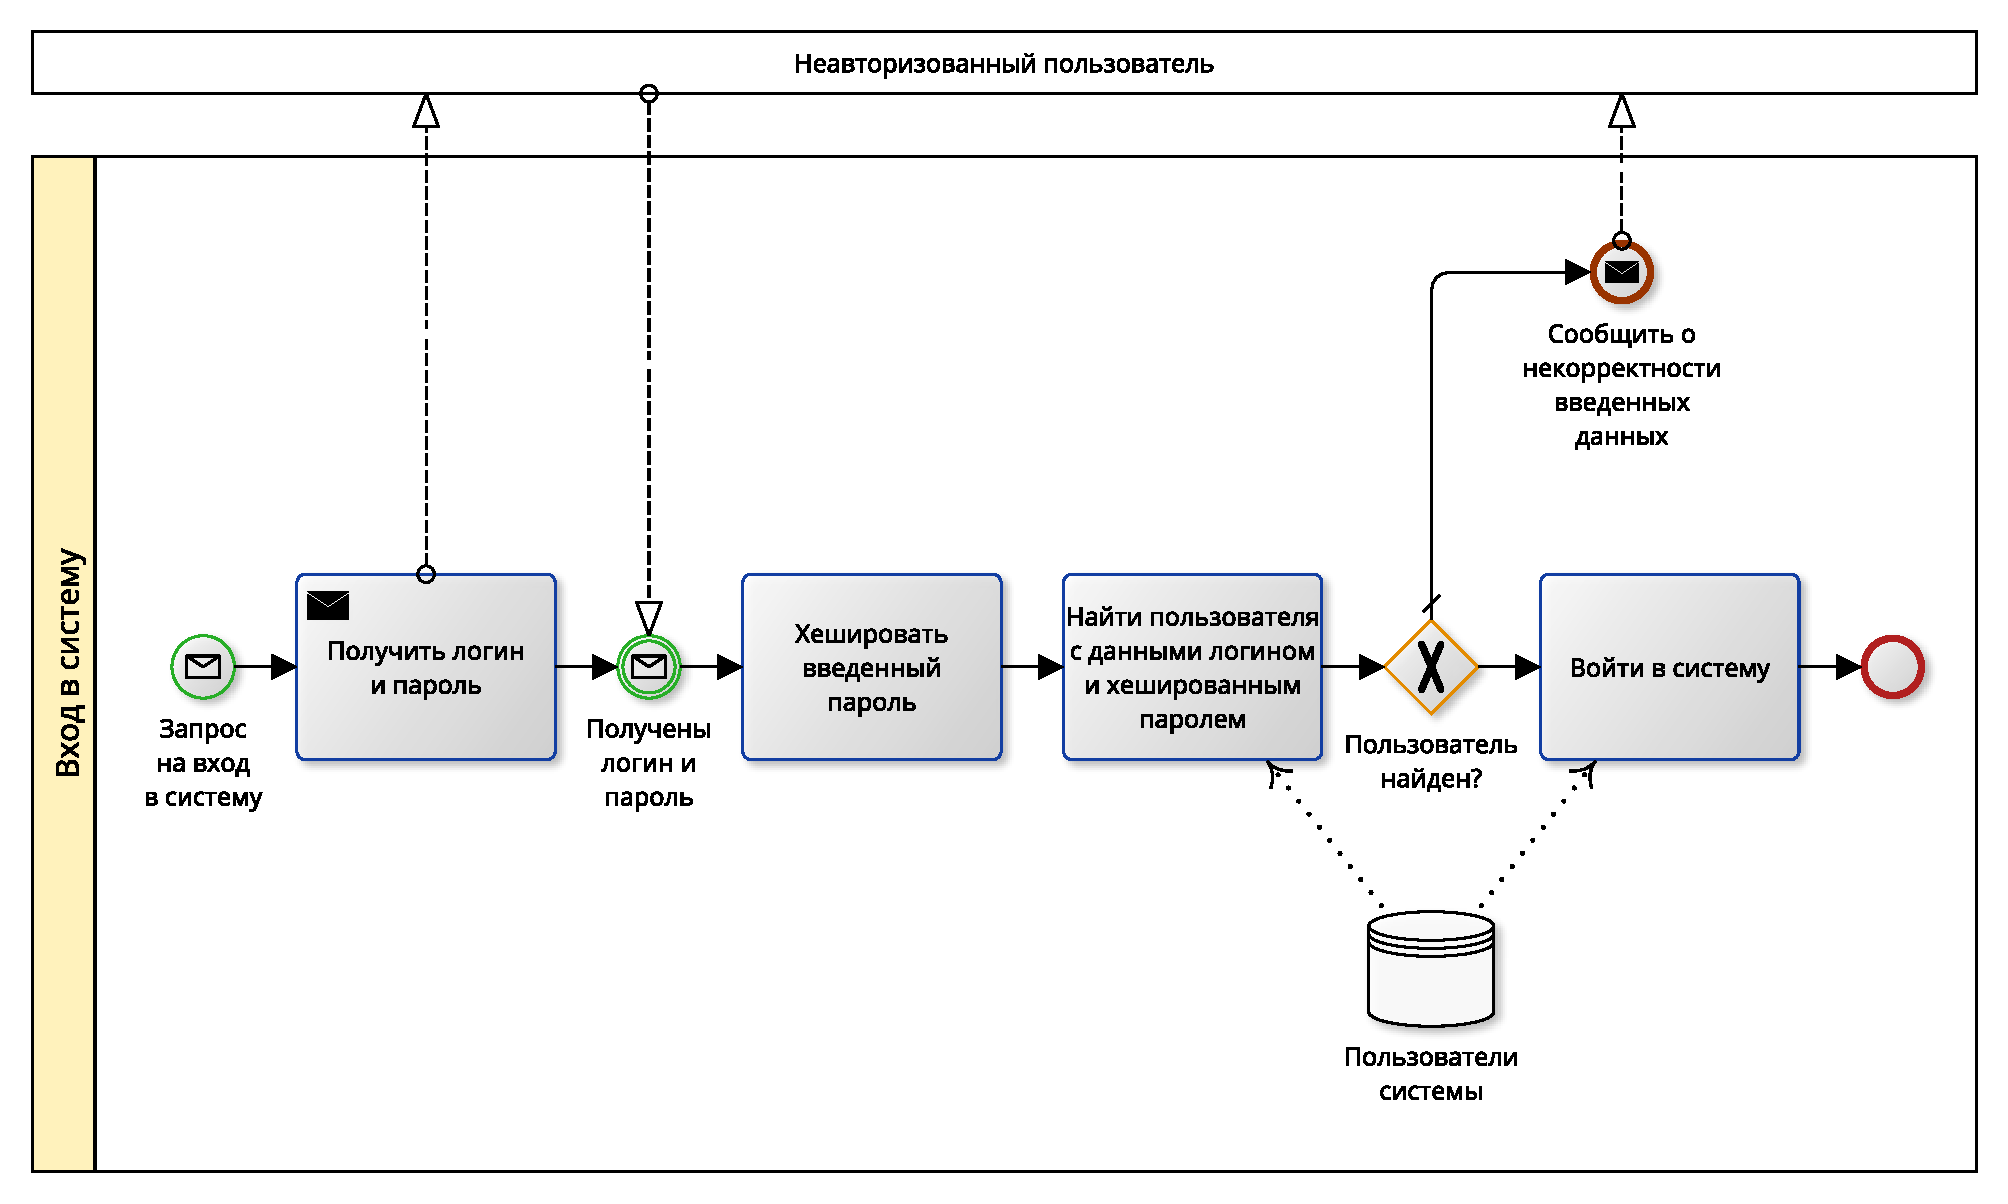
\includegraphics[width=0.8\linewidth]{bpmn_signin}
	\caption{Бизнес-правило входа в систему}
	\label{bpmn_signin}
\end{figure}
\begin{figure}[H]
	\centering
	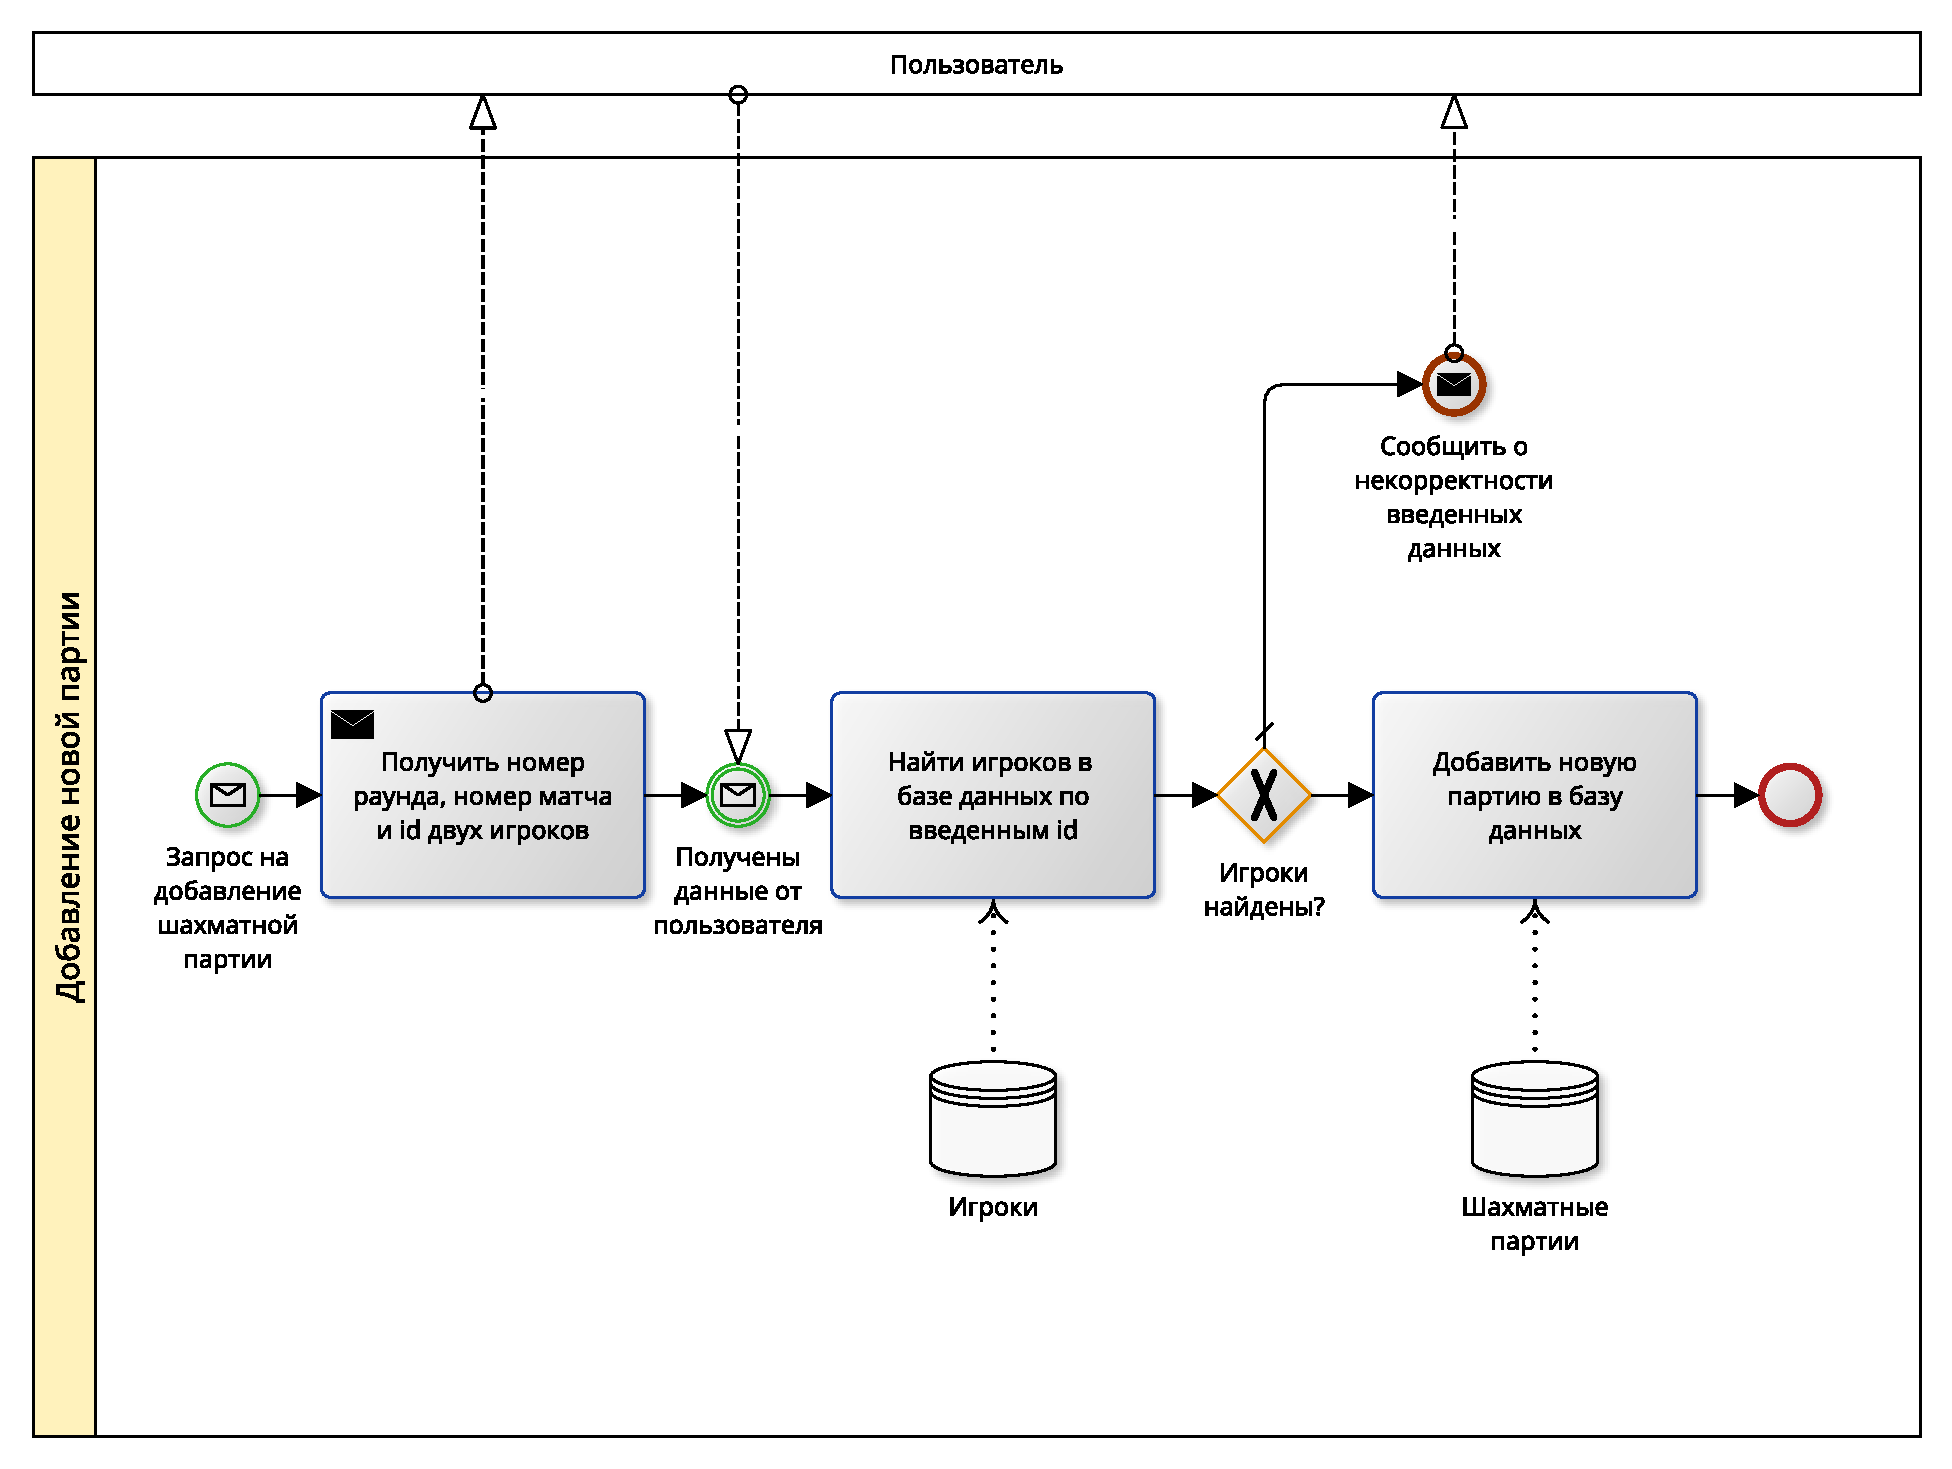
\includegraphics[width=\linewidth]{bpmn_newgame}
	\caption{Бизнес-правило добавления новой шахматной партии}
	\label{bpmn_newgame}
\end{figure}
\begin{figure}[H]
	\centering
	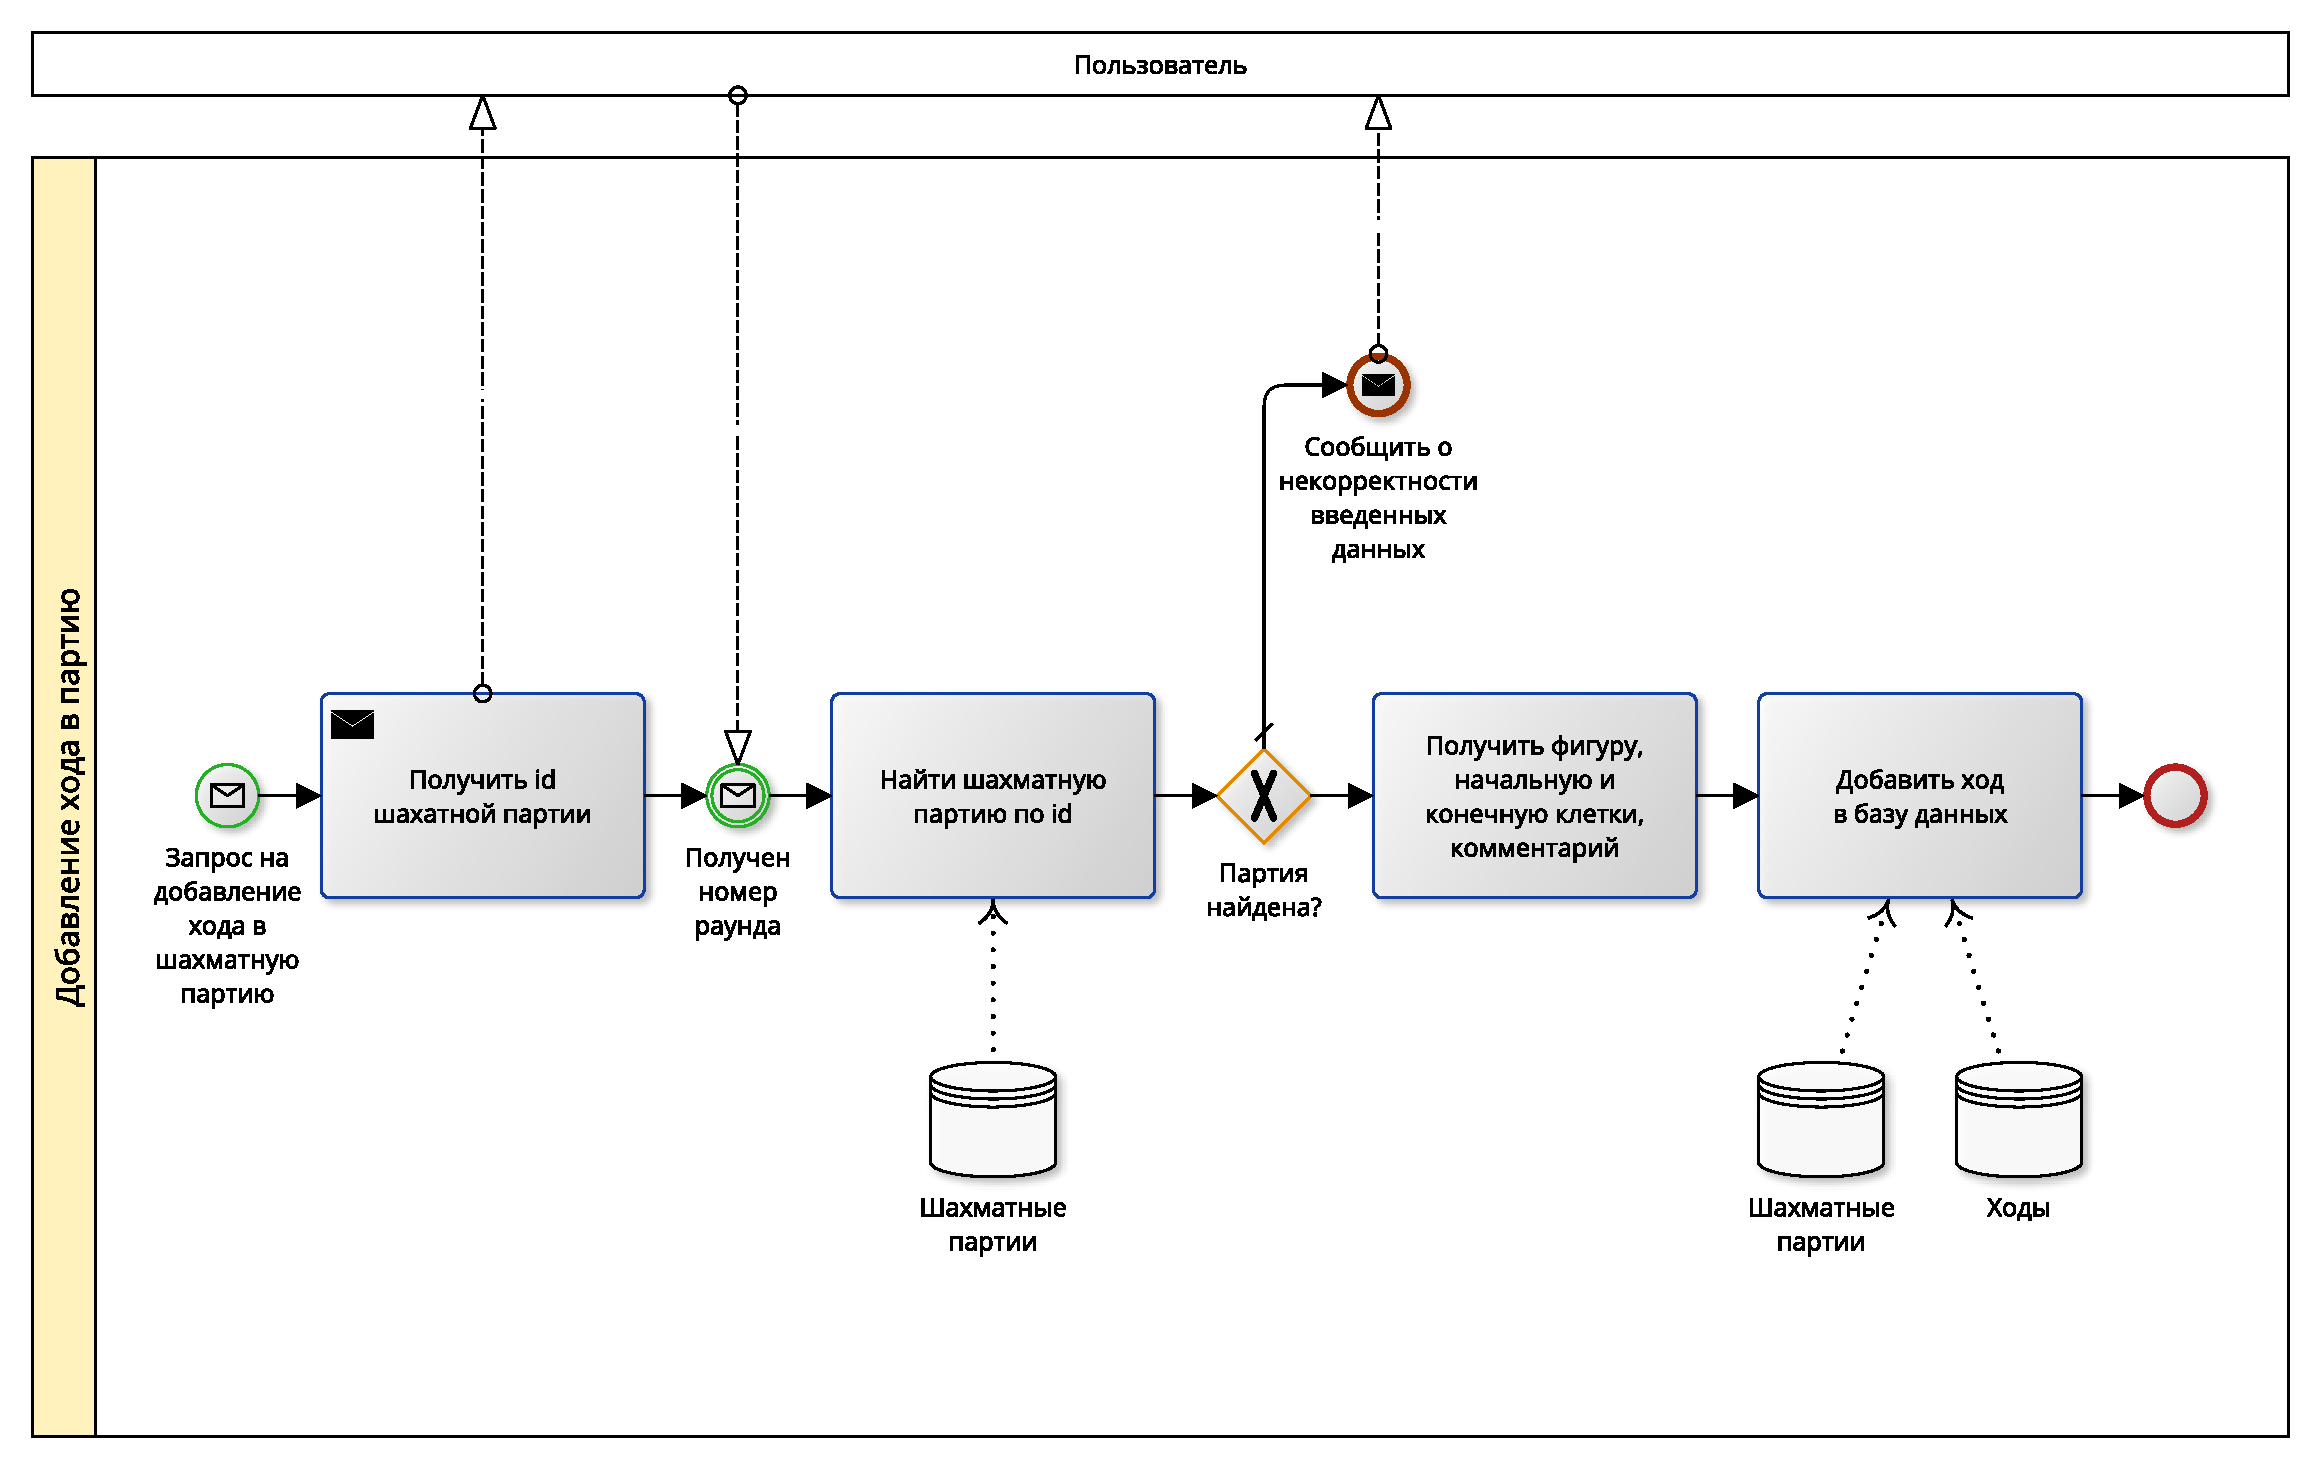
\includegraphics[width=\linewidth]{bpmn_addmove}
	\caption{Бизнес-правило добавления нового хода в партию}
	\label{bpmn_addmove}
\end{figure}
\begin{figure}[H]
	\centering
	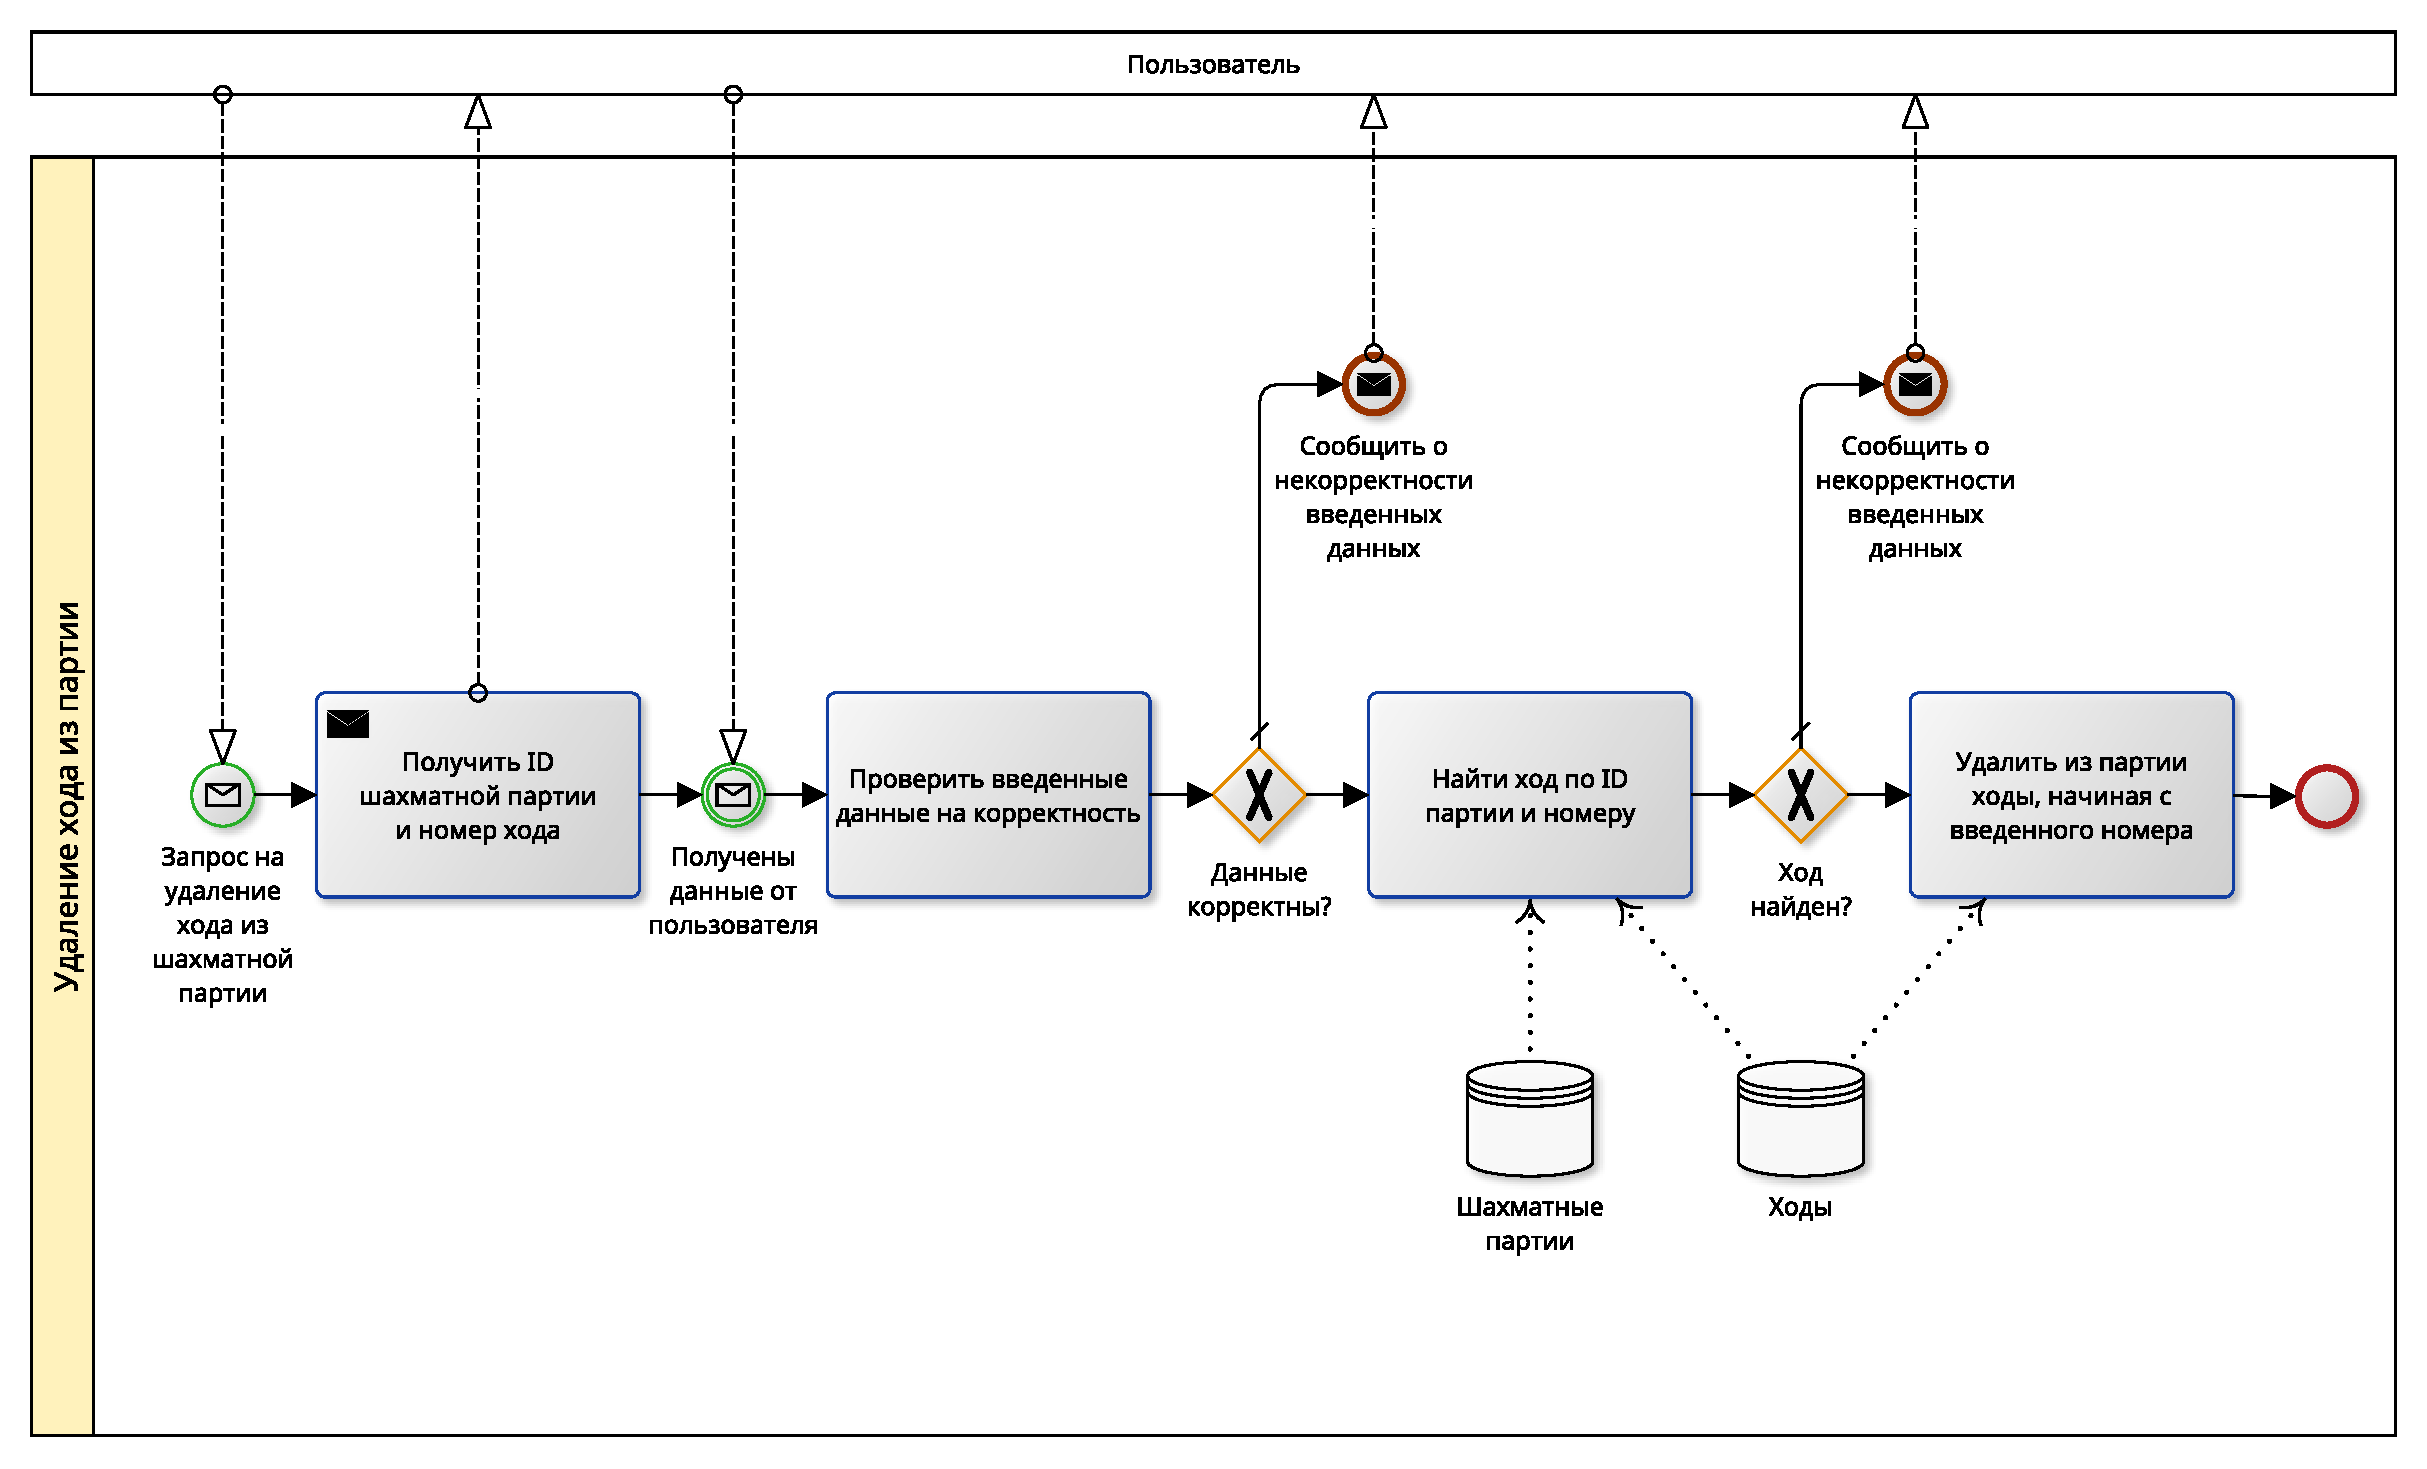
\includegraphics[width=\linewidth]{bpmn_removemove}
	\caption{Бизнес-правило удаления хода из партии}
	\label{bpmn_removemove}
\end{figure}
\begin{figure}[H]
	\centering
	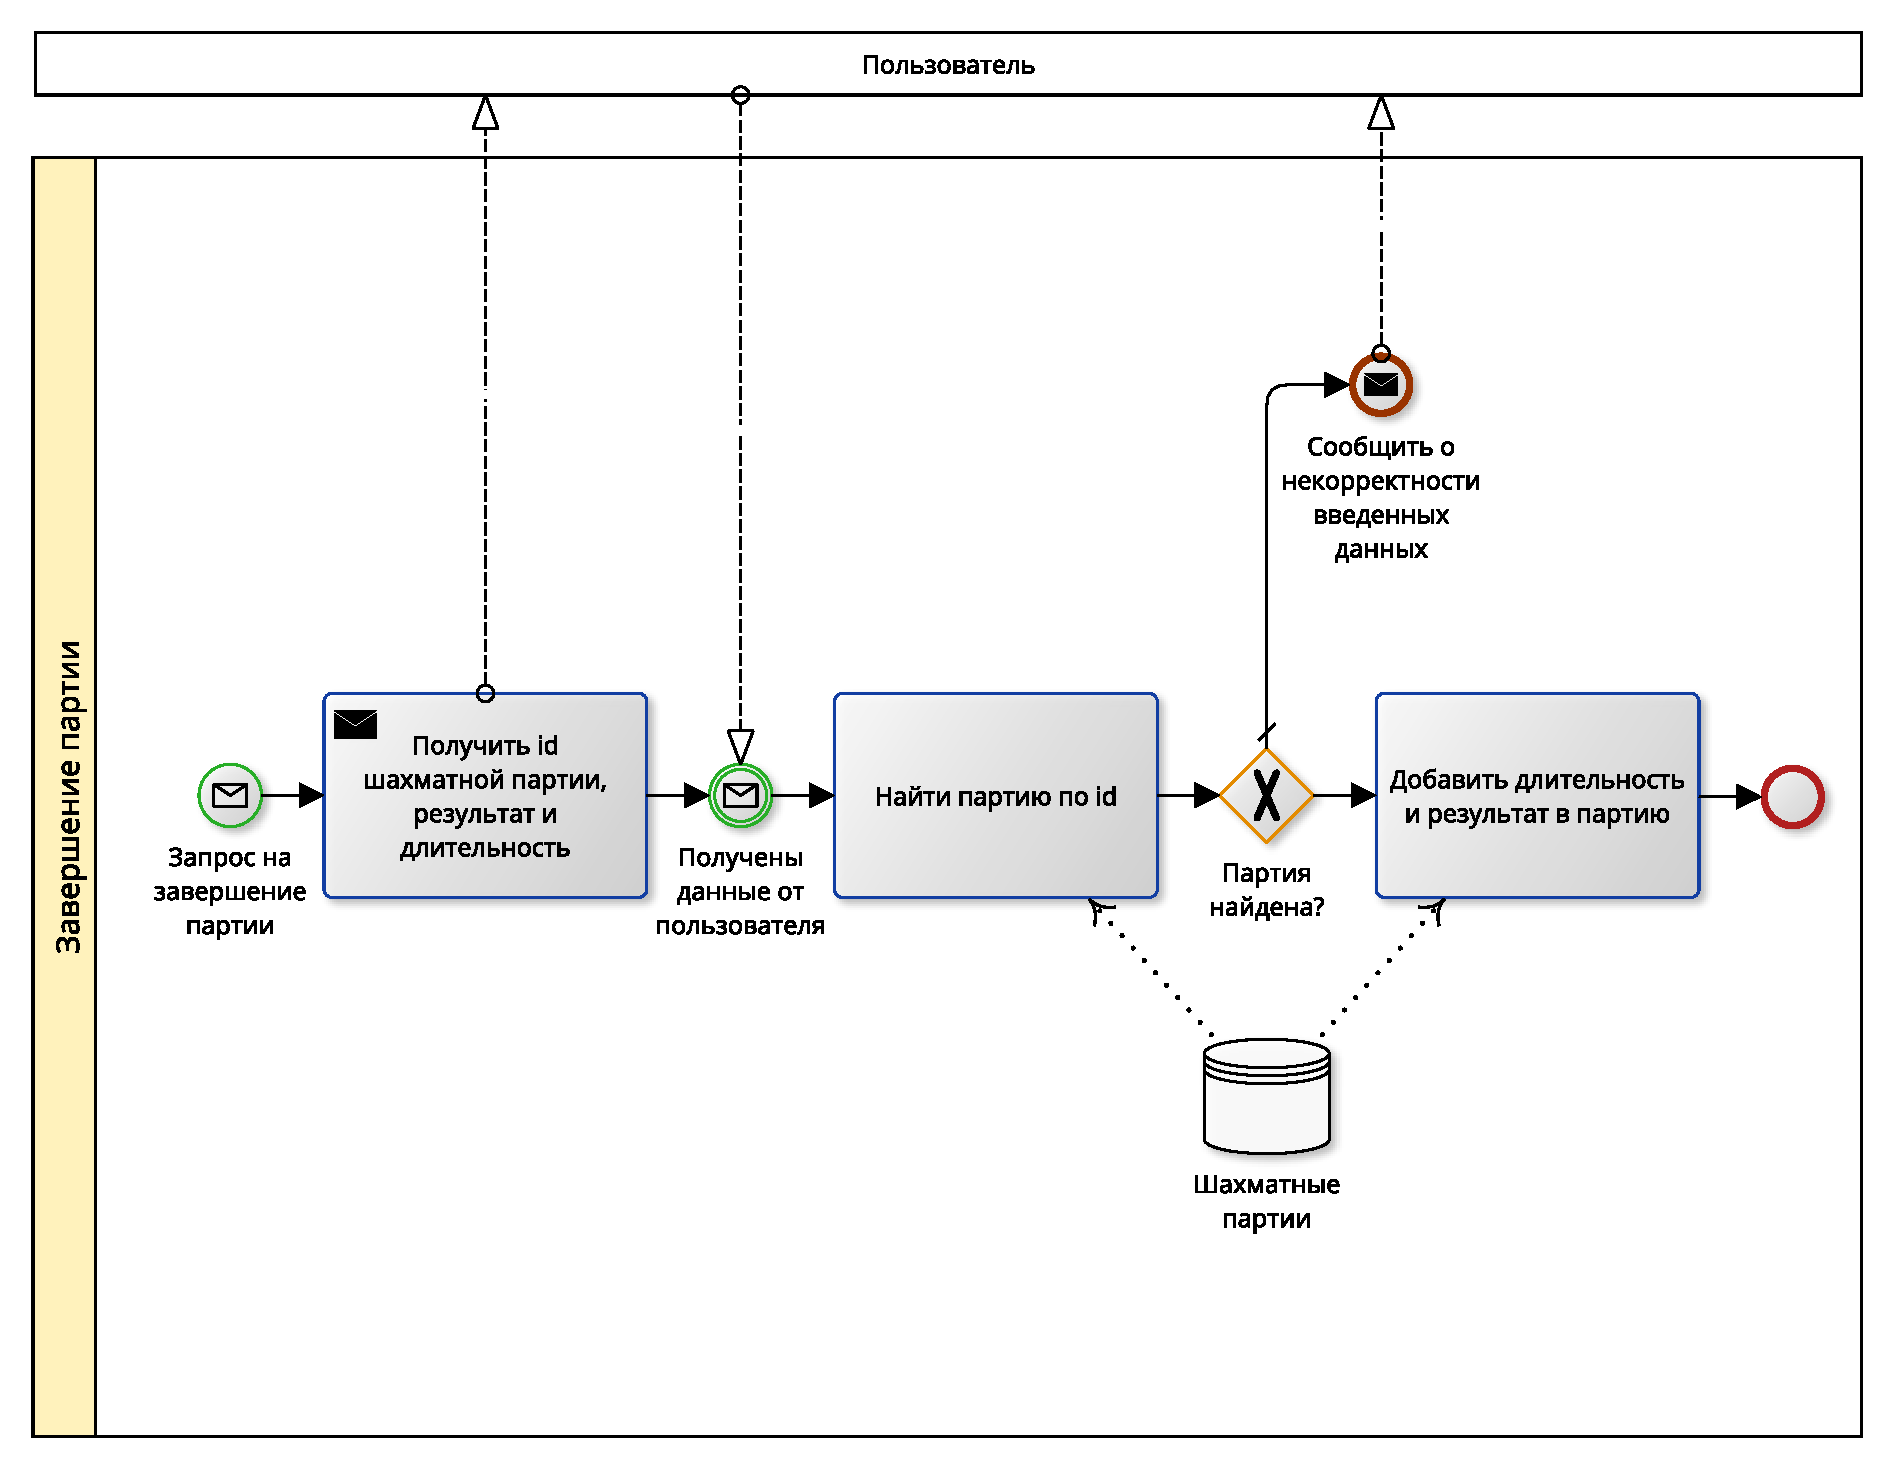
\includegraphics[width=\linewidth]{bpmn_endgame}
	\caption{Бизнес-правило завершения партии}
	\label{bpmn_endgame}
\end{figure}
\begin{figure}[H]
	\centering
	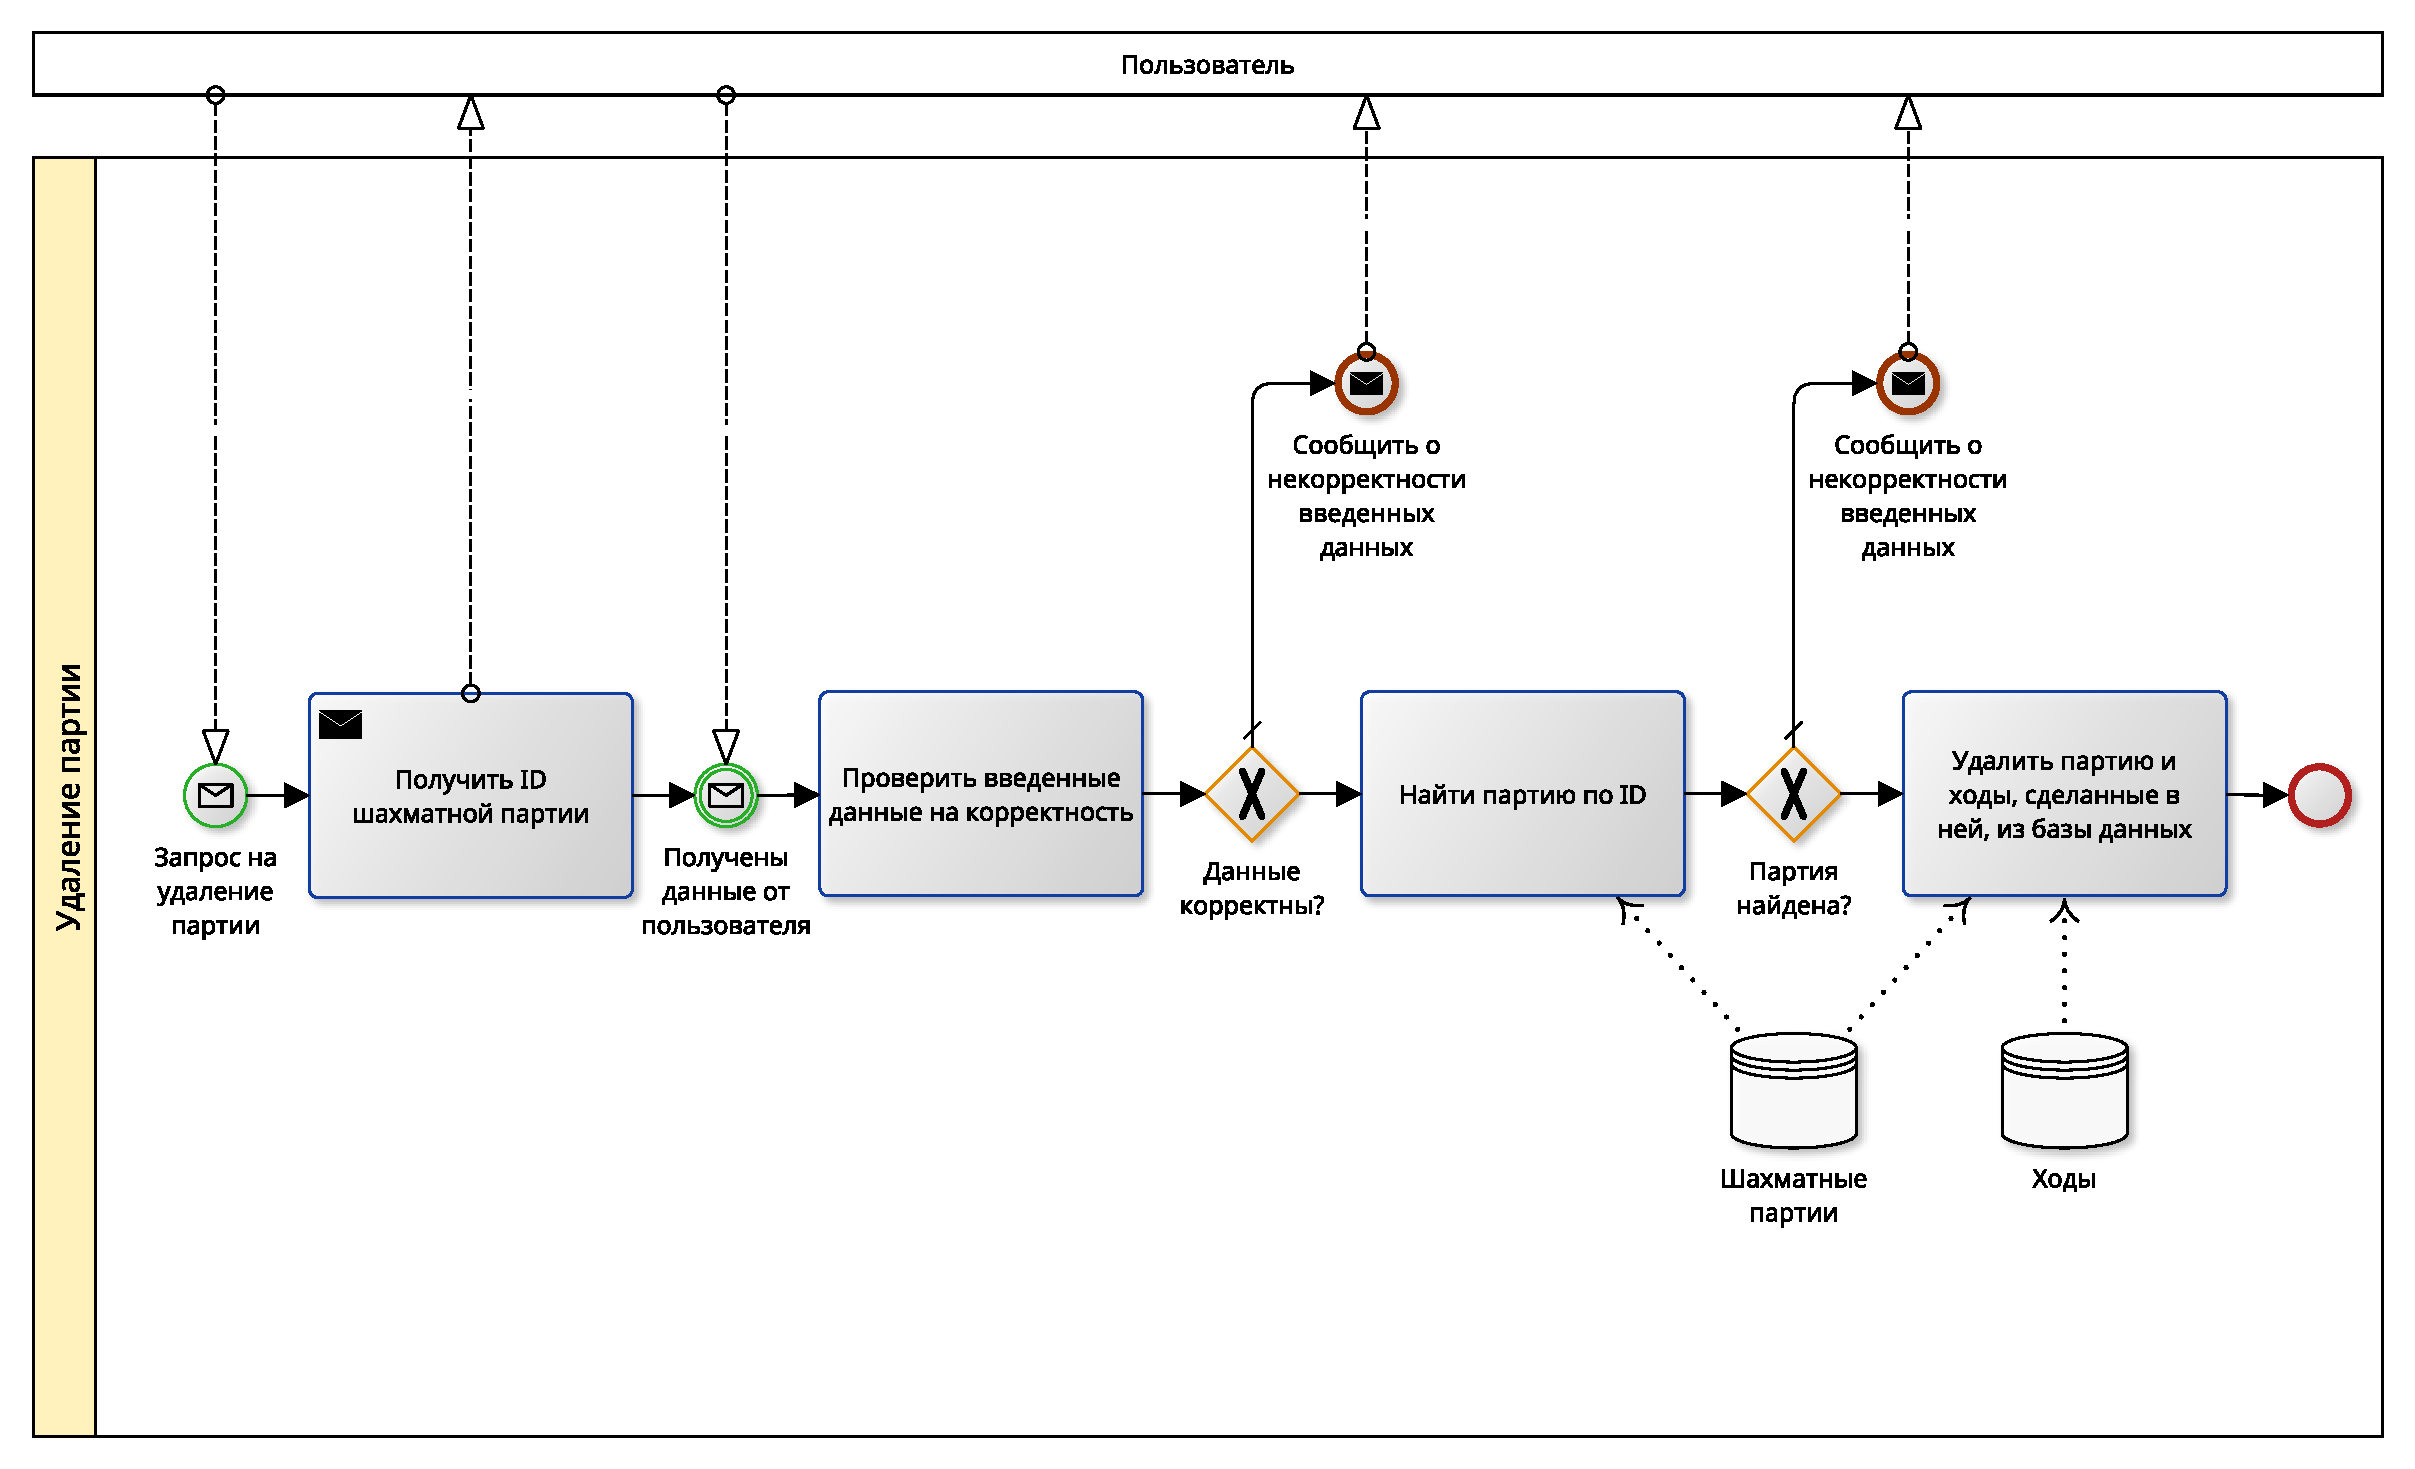
\includegraphics[width=\linewidth]{bpmn_removegame}
	\caption{Бизнес-правило удаления партии}
	\label{bpmn_removegame}
\end{figure}
\begin{figure}[H]
	\centering
	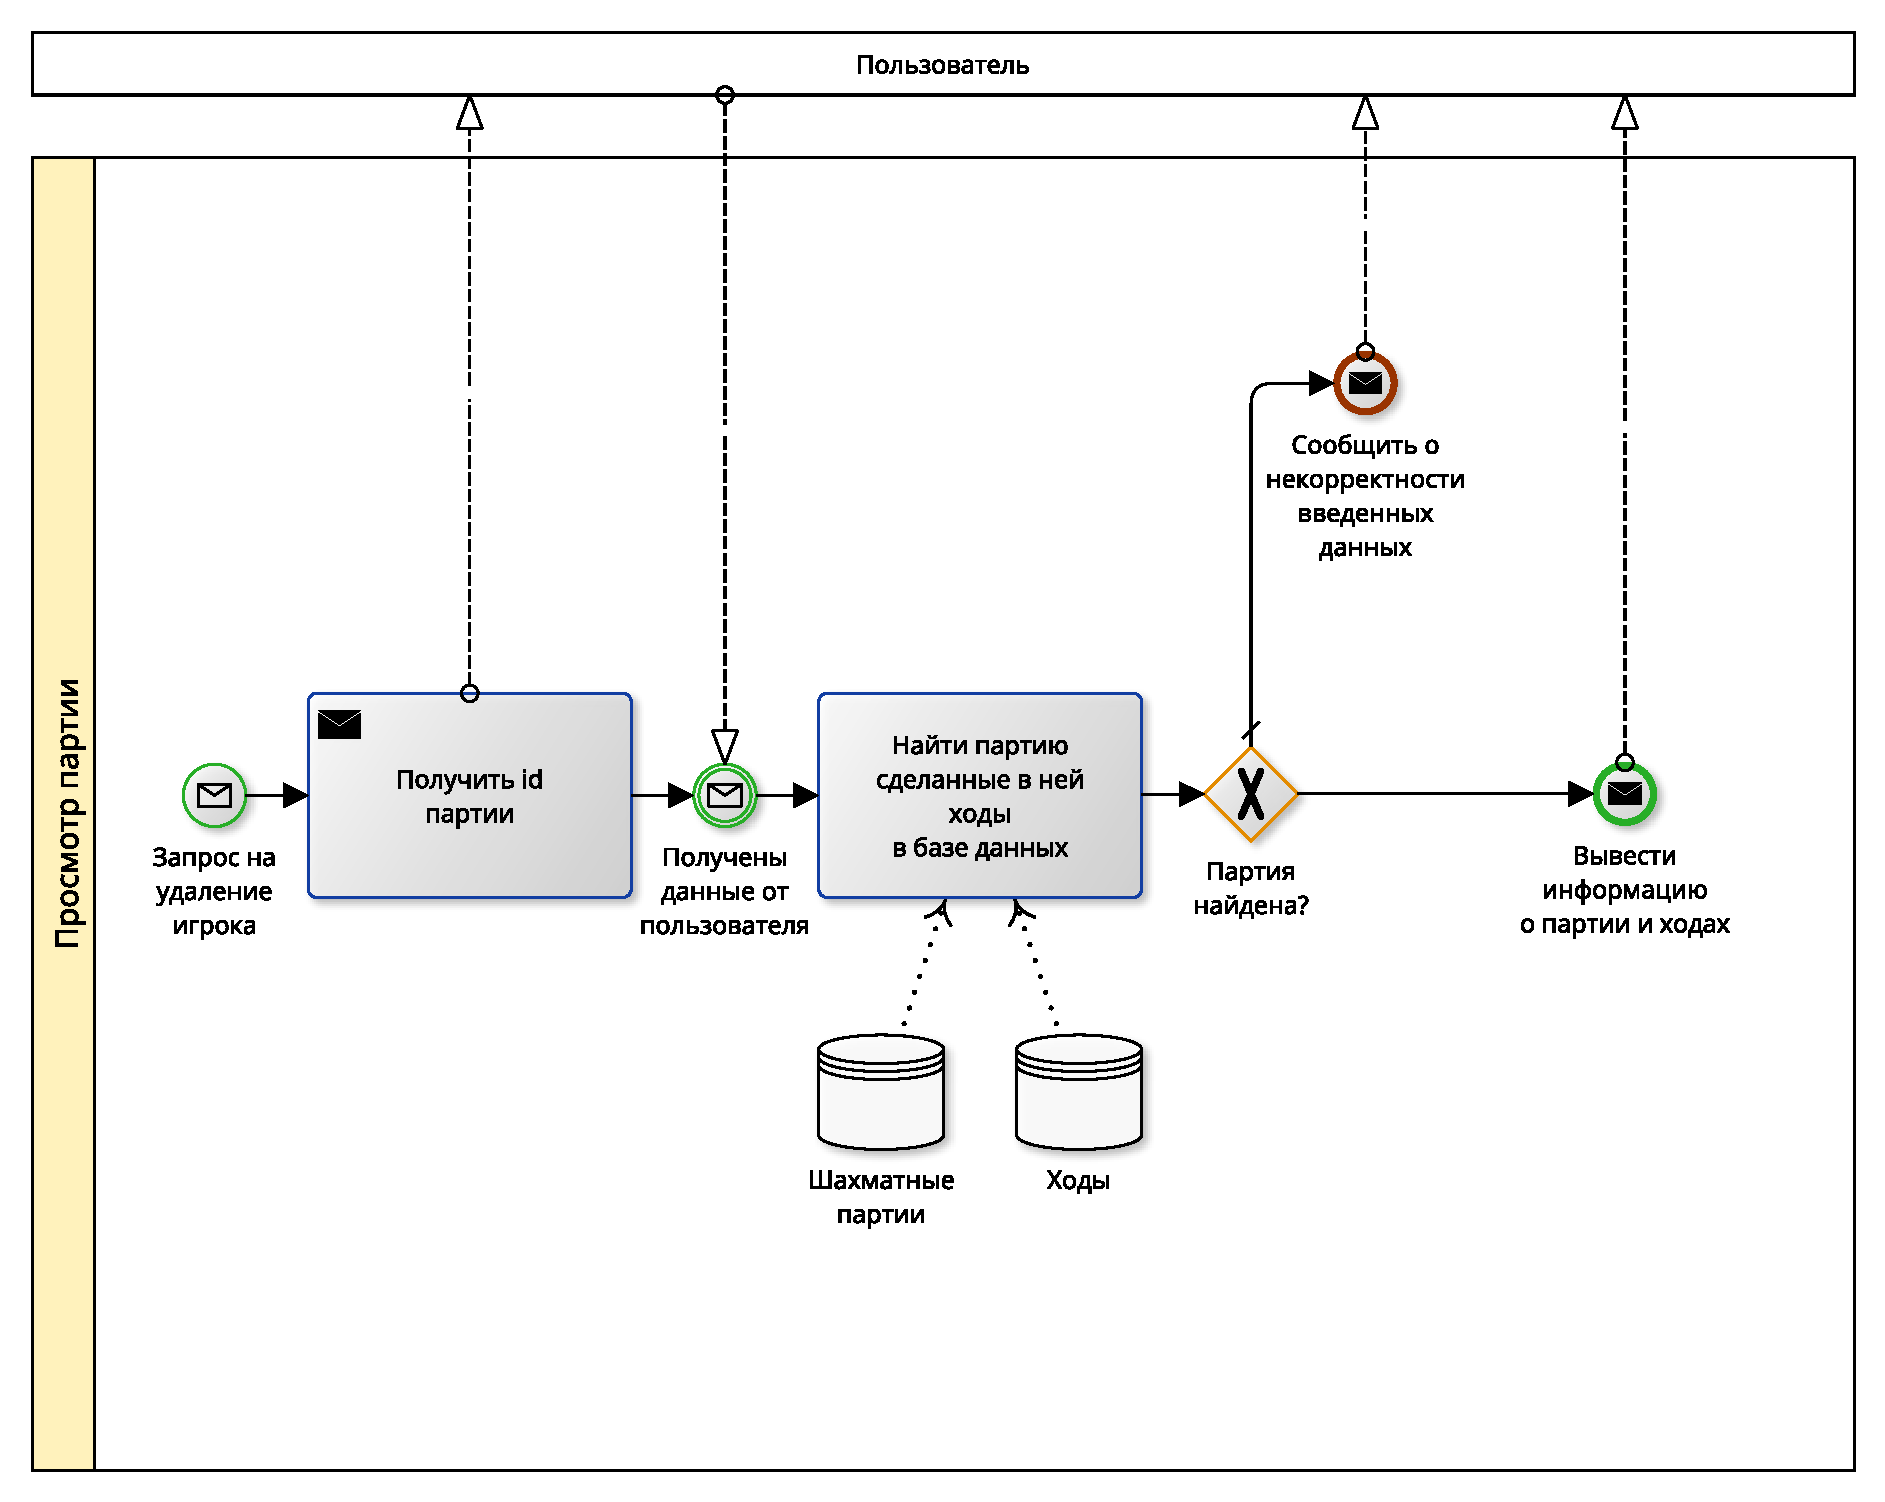
\includegraphics[width=\linewidth]{bpmn_showgame}
	\caption{Бизнес-правило просмотра партии}
	\label{bpmn_showgame}
\end{figure}
\begin{figure}[H]
	\centering
	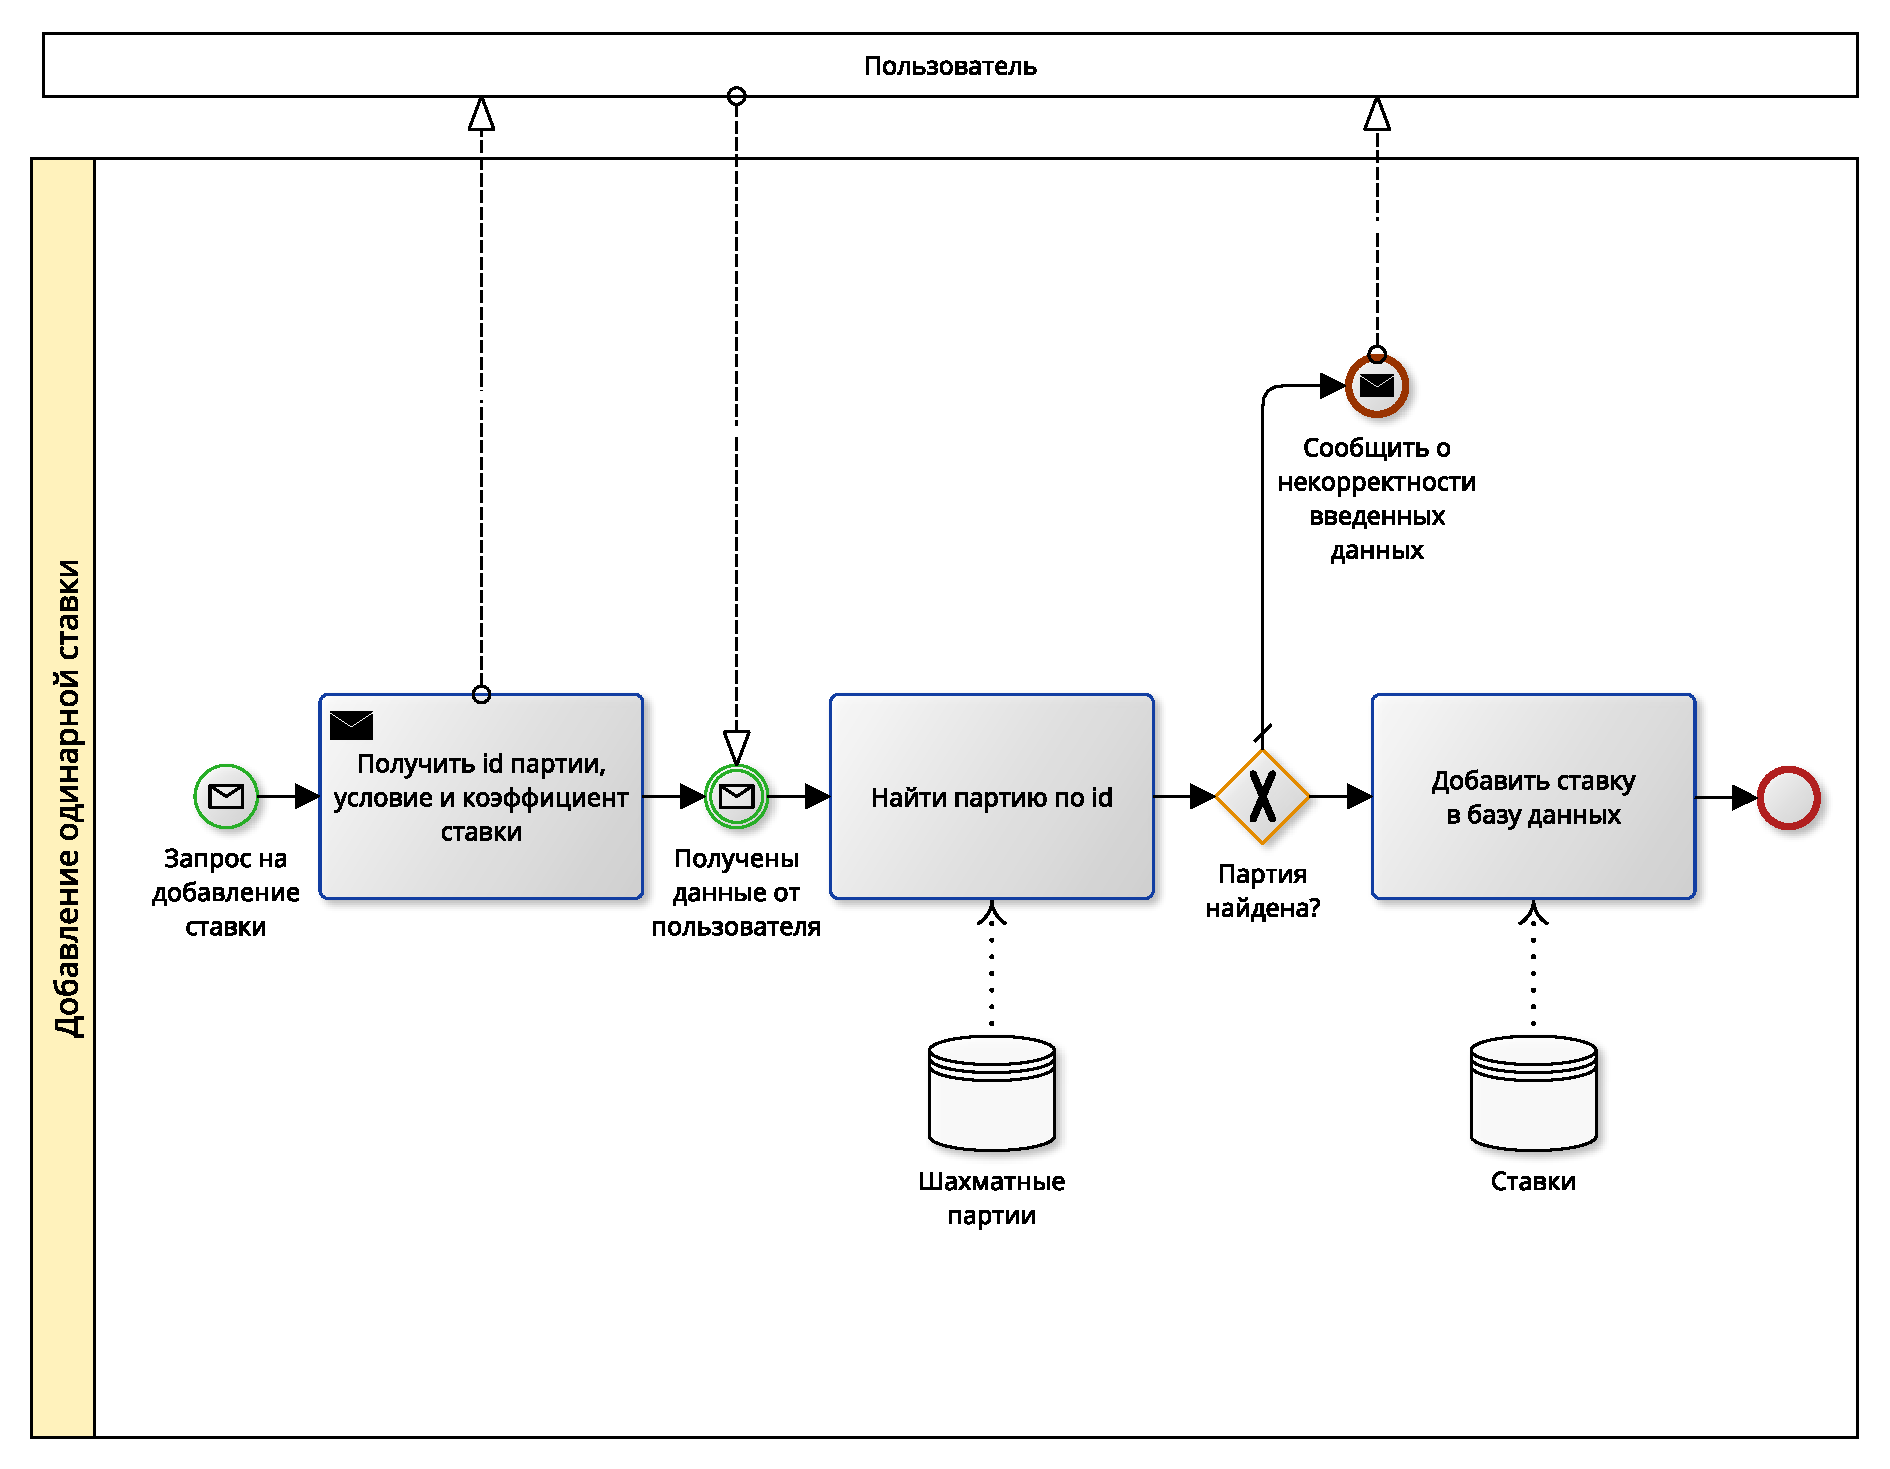
\includegraphics[width=\linewidth]{bpmn_addelembet}
	\caption{Бизнес-правило добавления одинарной ставки}
	\label{bpmn_addelembet}
\end{figure}
\begin{figure}[H]
	\centering
	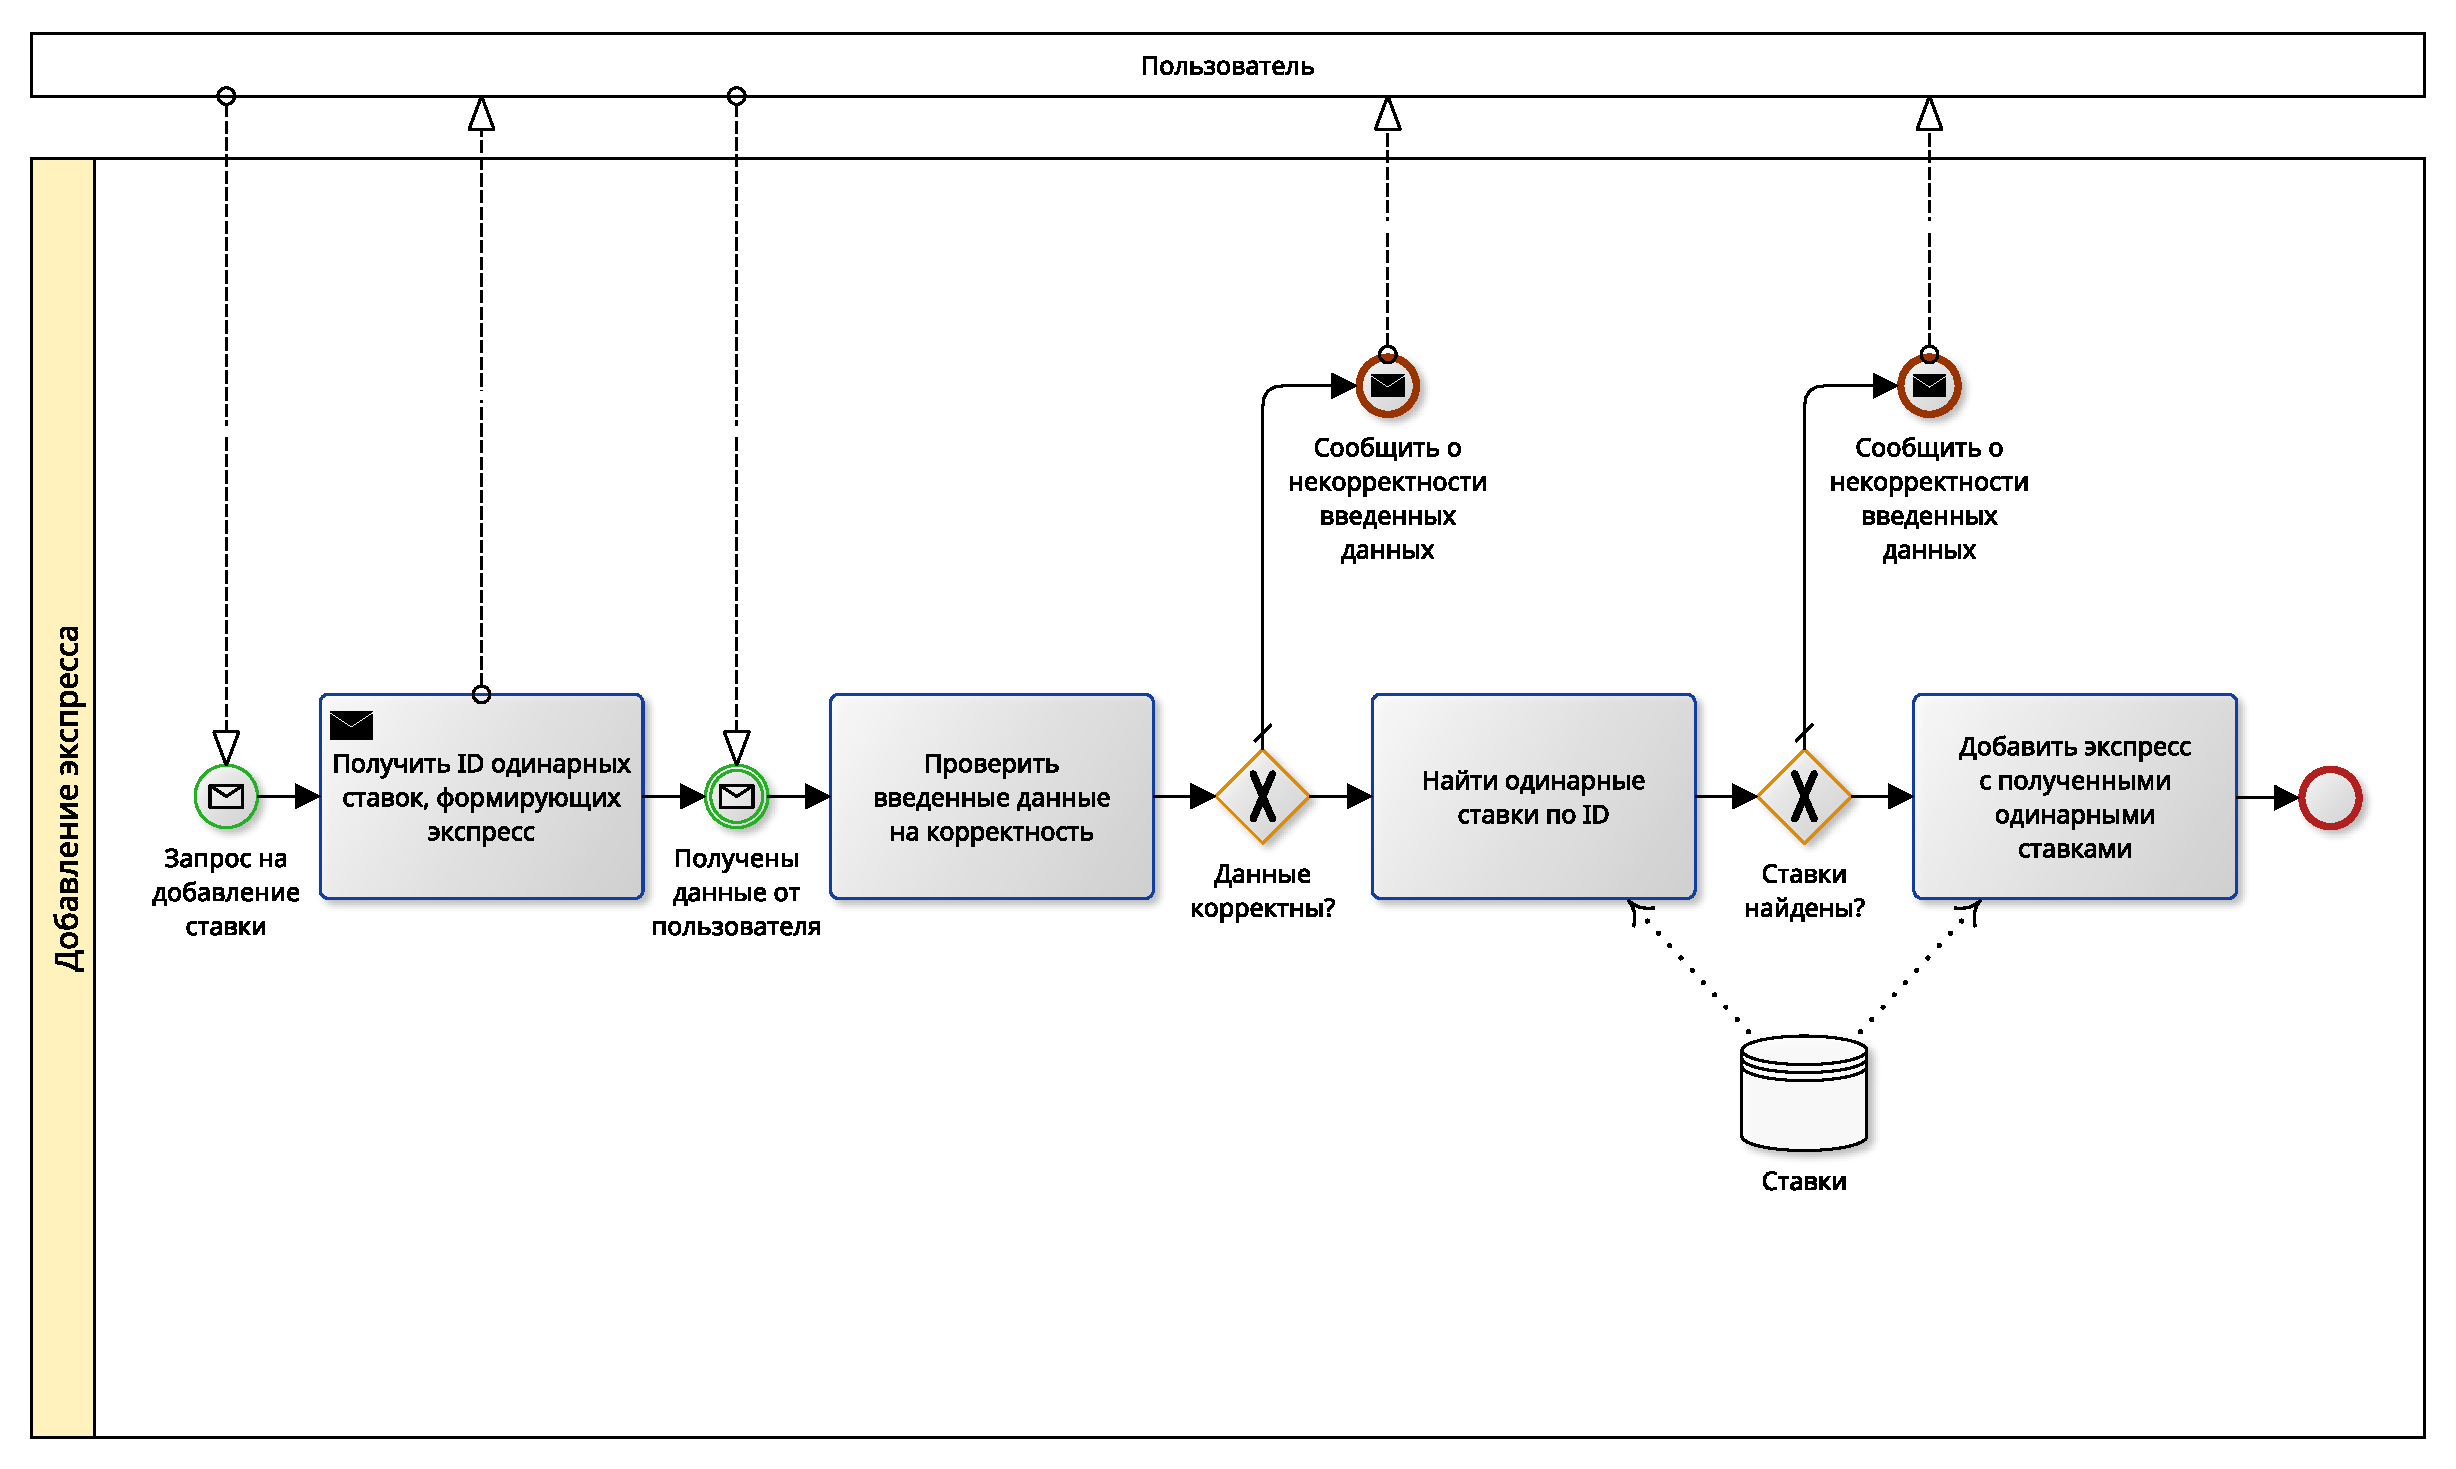
\includegraphics[width=\linewidth]{bpmn_addexpress}
	\caption{Бизнес-правило добавления экспресса}
	\label{bpmn_addexpress}
\end{figure}
\begin{figure}[H]
	\centering
	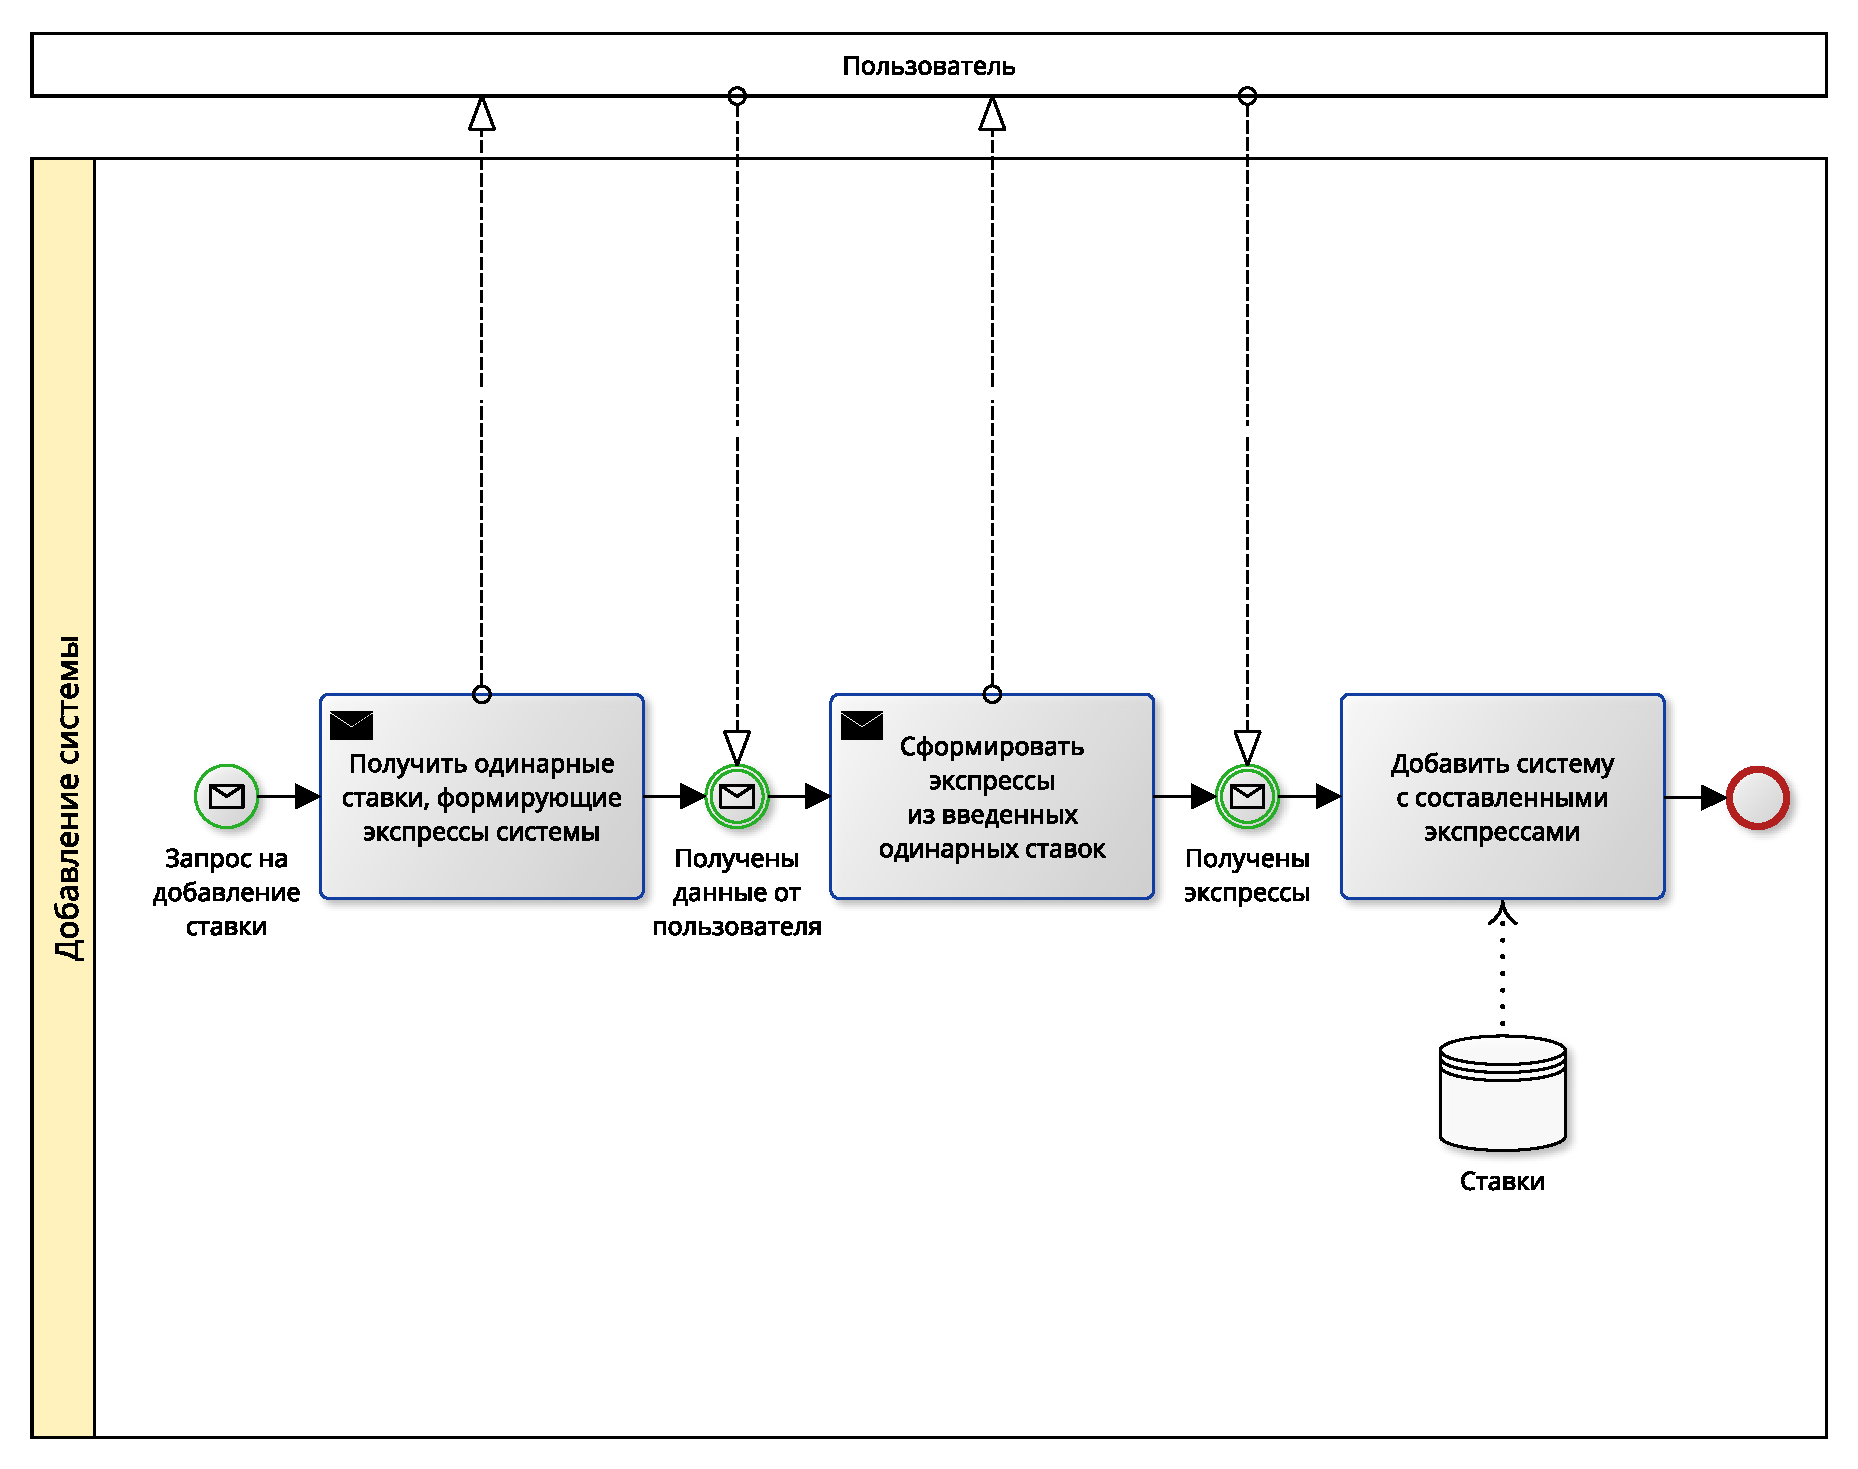
\includegraphics[width=\linewidth]{bpmn_addsystem}
	\caption{Бизнес-правило добавления системы}
	\label{bpmn_addsystem}
\end{figure}
\begin{figure}[H]
	\centering
	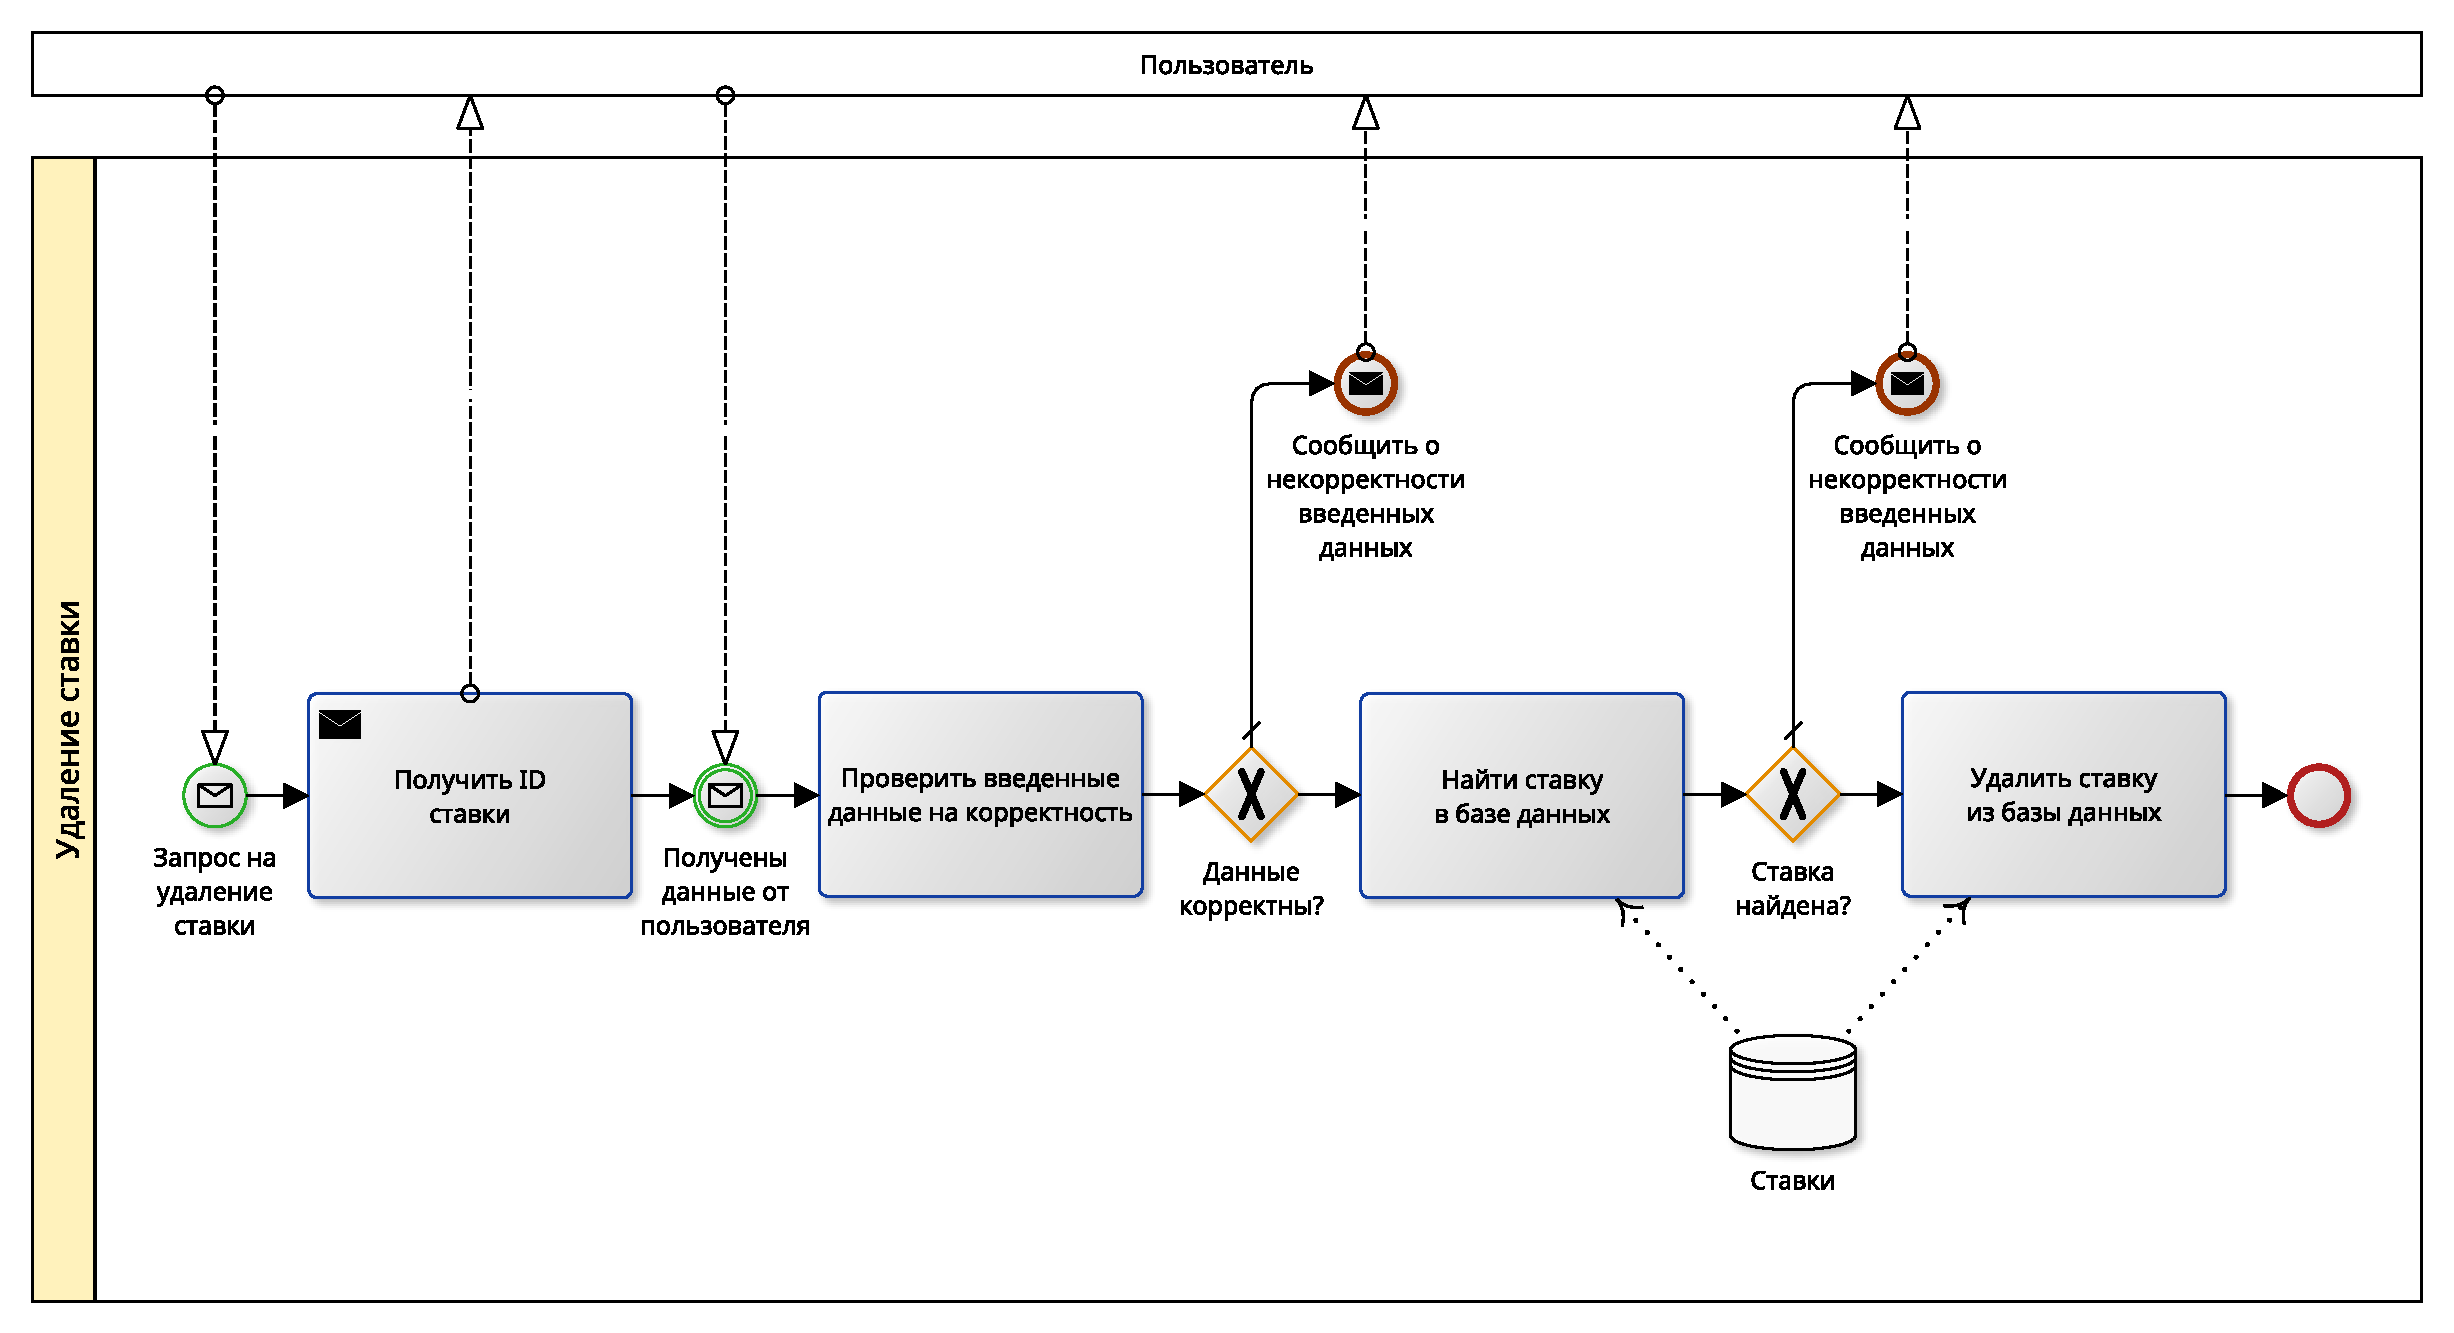
\includegraphics[width=\linewidth]{bpmn_removebet}
	\caption{Бизнес-правило удаления ставки}
	\label{bpmn_removebet}
\end{figure}
\begin{figure}[H]
	\centering
	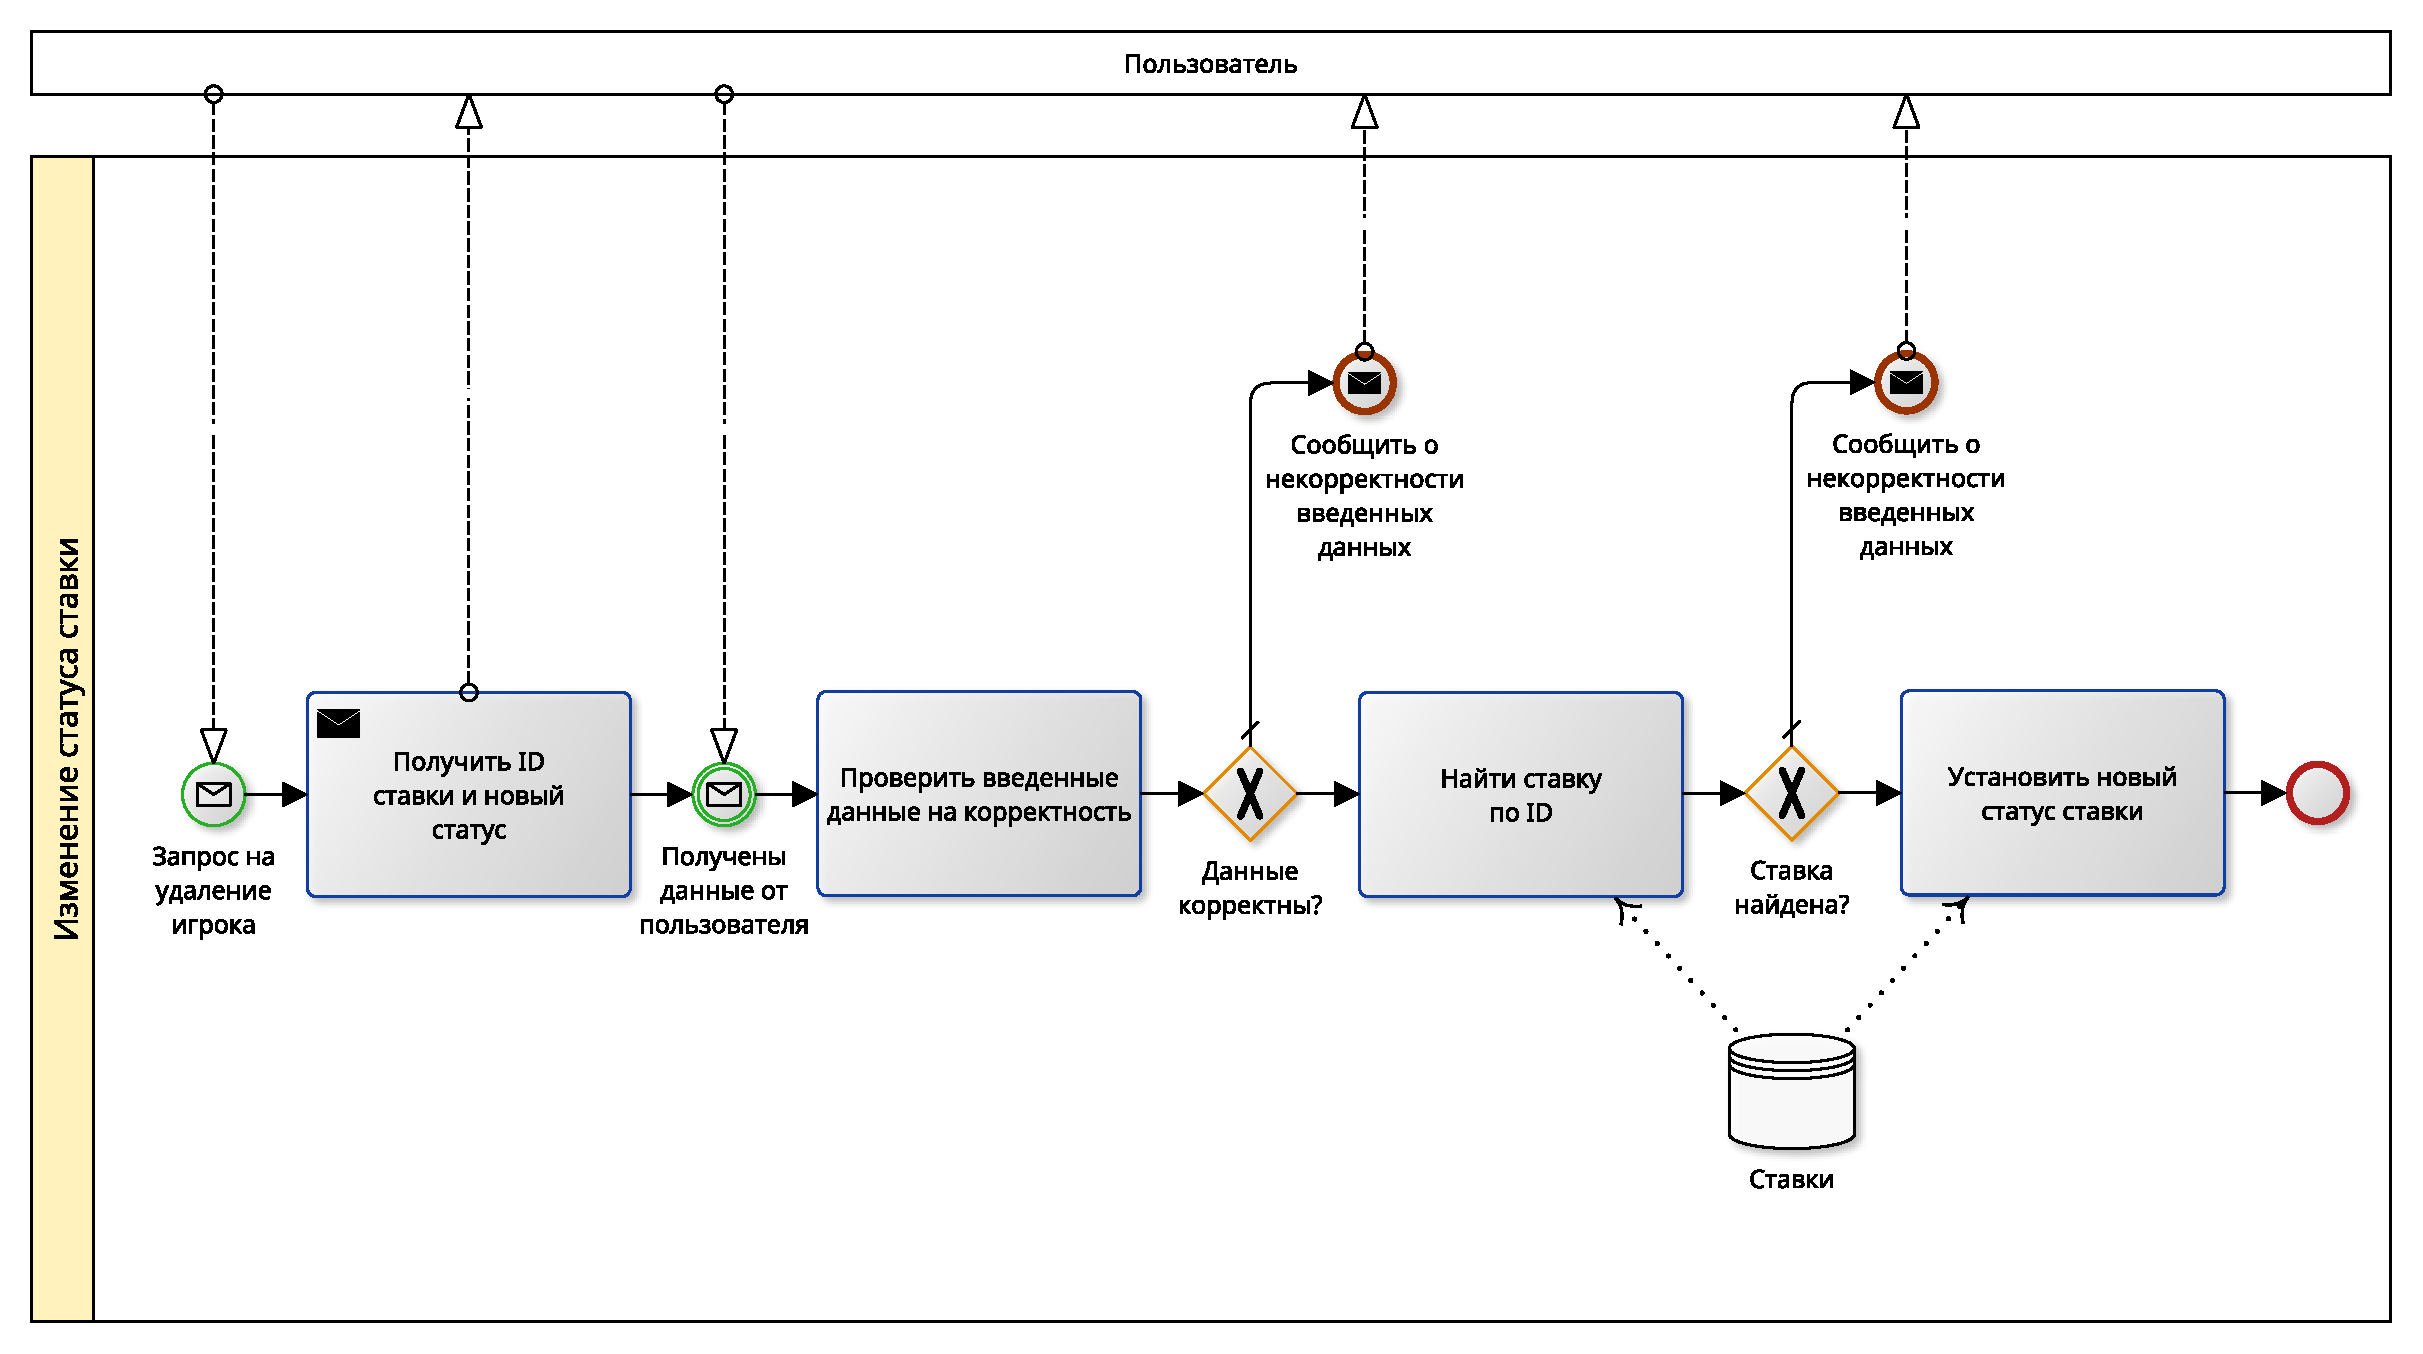
\includegraphics[width=\linewidth]{bpmn_setbetstatus}
	\caption{Бизнес-правило изменения статуса ставки}
	\label{bpmn_setbetstatus}
\end{figure}
\begin{figure}[H]
	\centering
	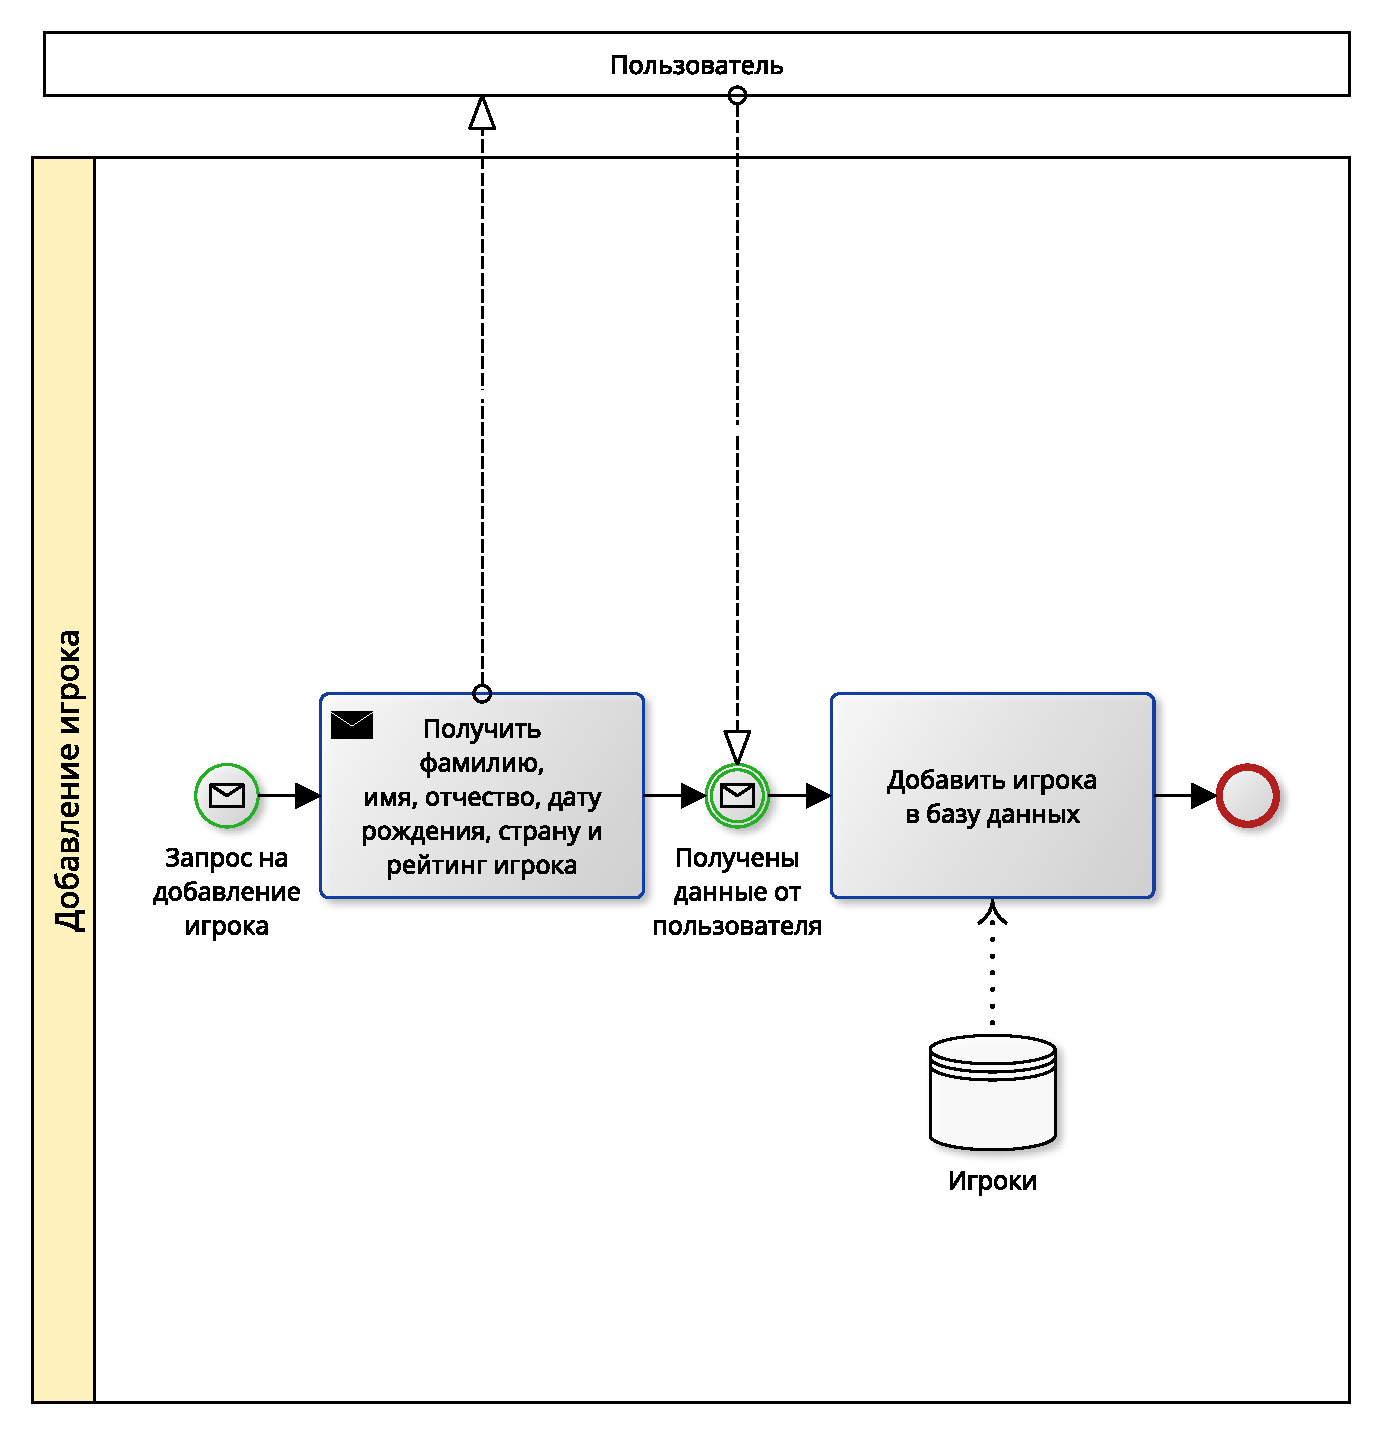
\includegraphics[width=\linewidth]{bpmn_addplayer}
	\caption{Бизнес-правило добавления игрока}
	\label{bpmn_addplayer}
\end{figure}
\begin{figure}[H]
	\centering
	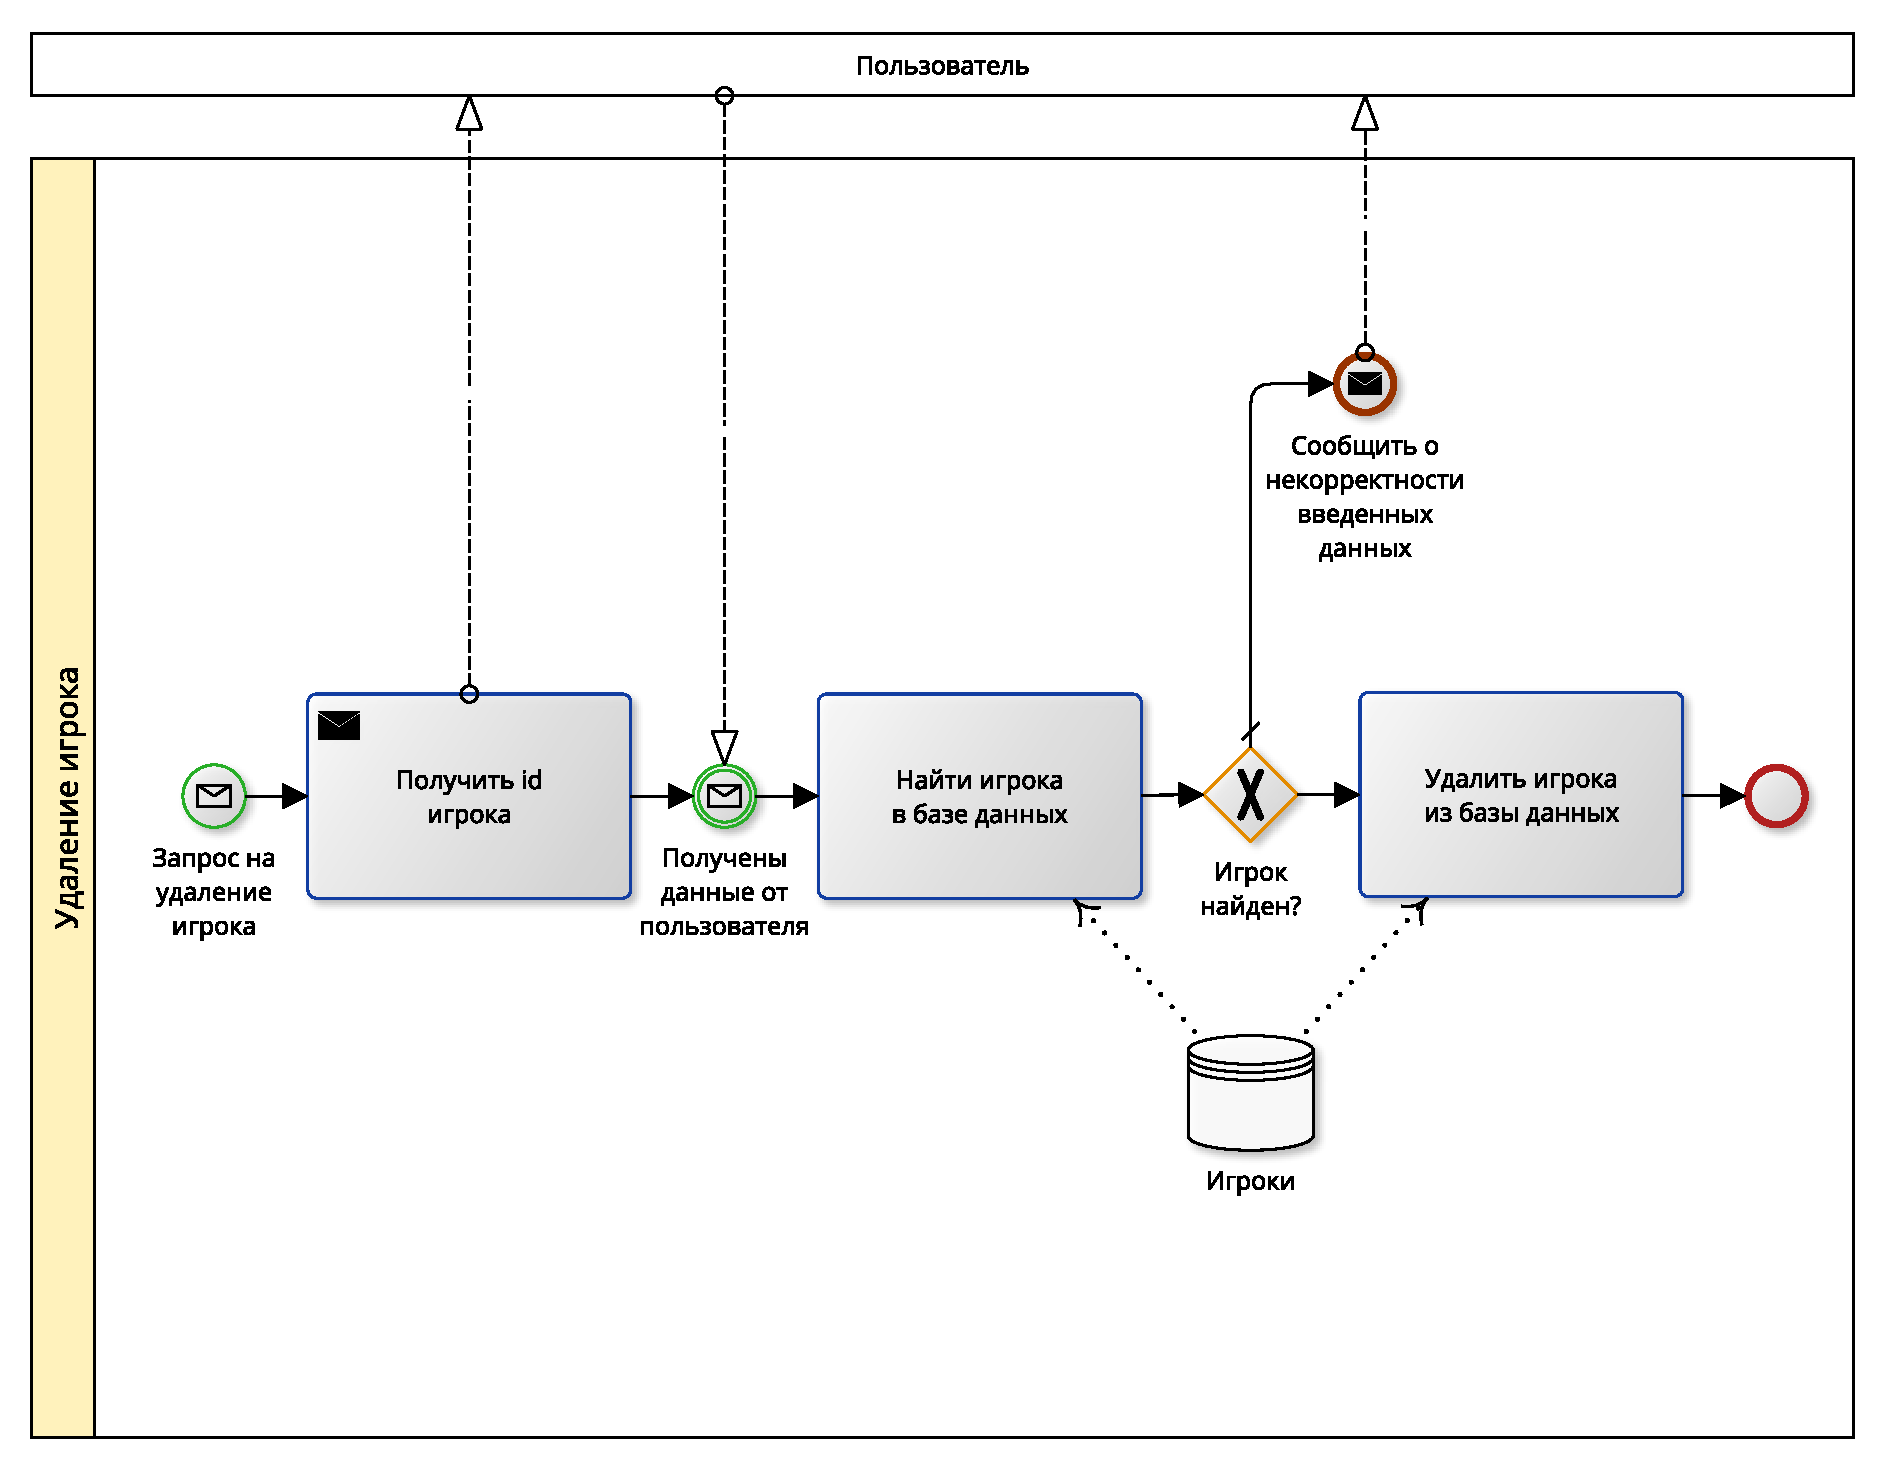
\includegraphics[width=\linewidth]{bpmn_removeplayer}
	\caption{Бизнес-правило удаления игрока}
	\label{bpmn_removeplayer}
\end{figure}
\begin{figure}[H]
	\centering
	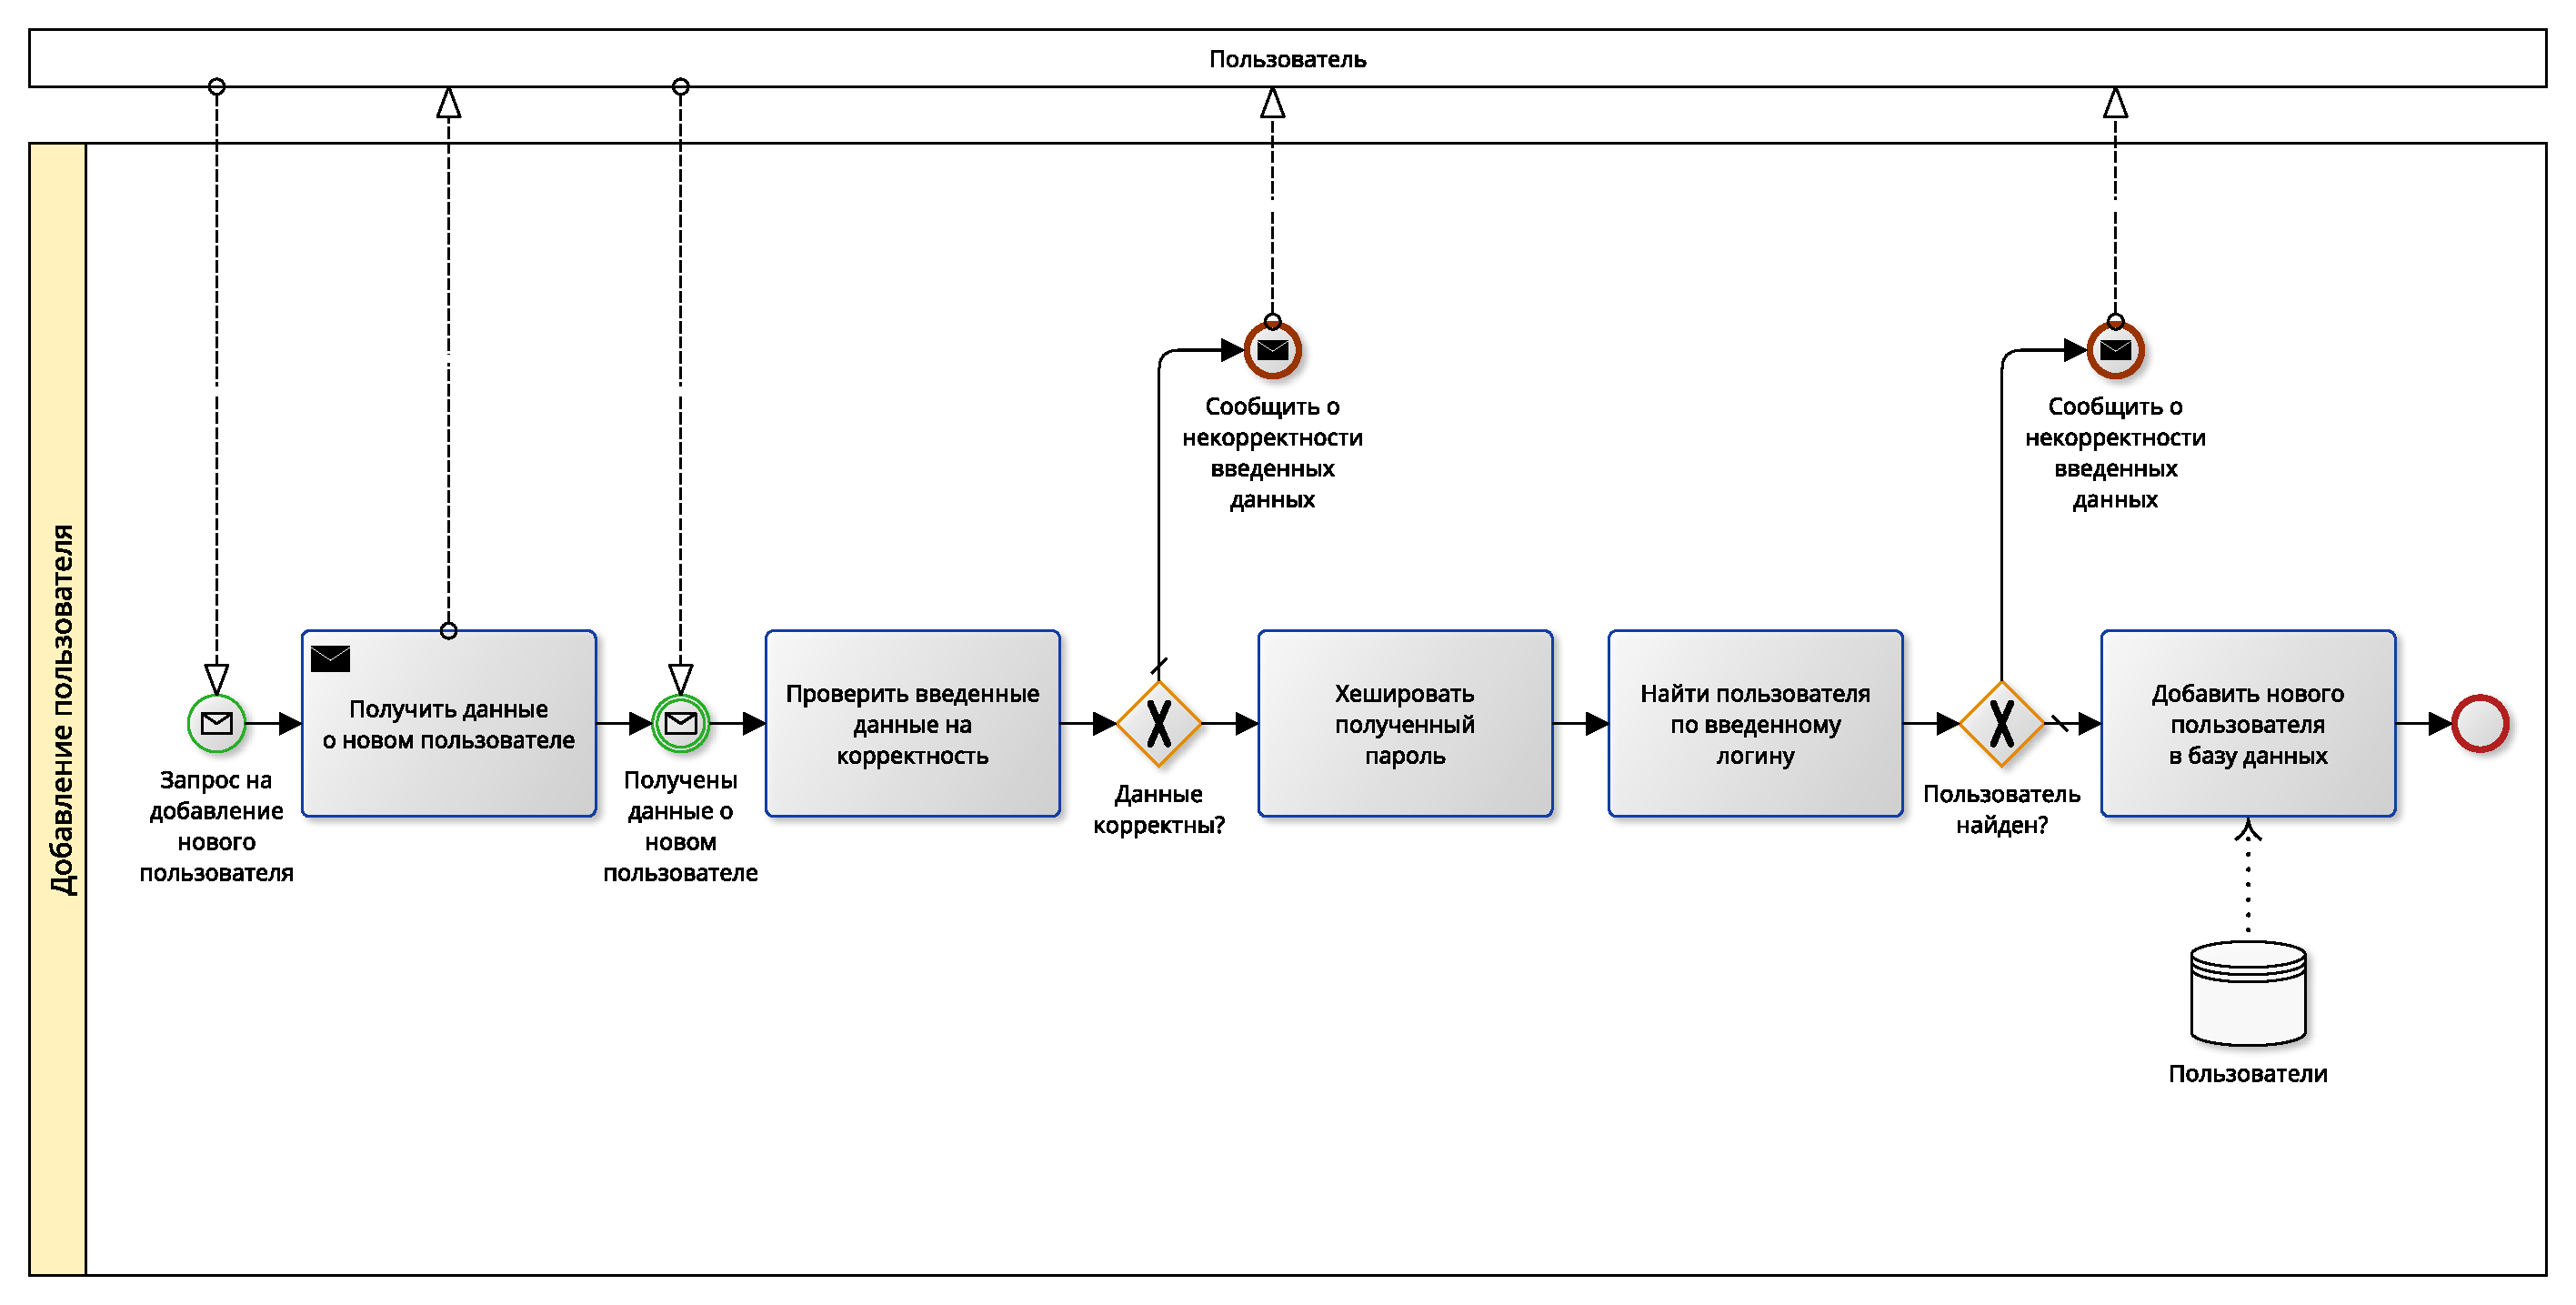
\includegraphics[width=\linewidth]{bpmn_adduser}
	\caption{Бизнес-правило добавления пользователя}
	\label{bpmn_adduser}
\end{figure}
\begin{figure}[H]
	\centering
	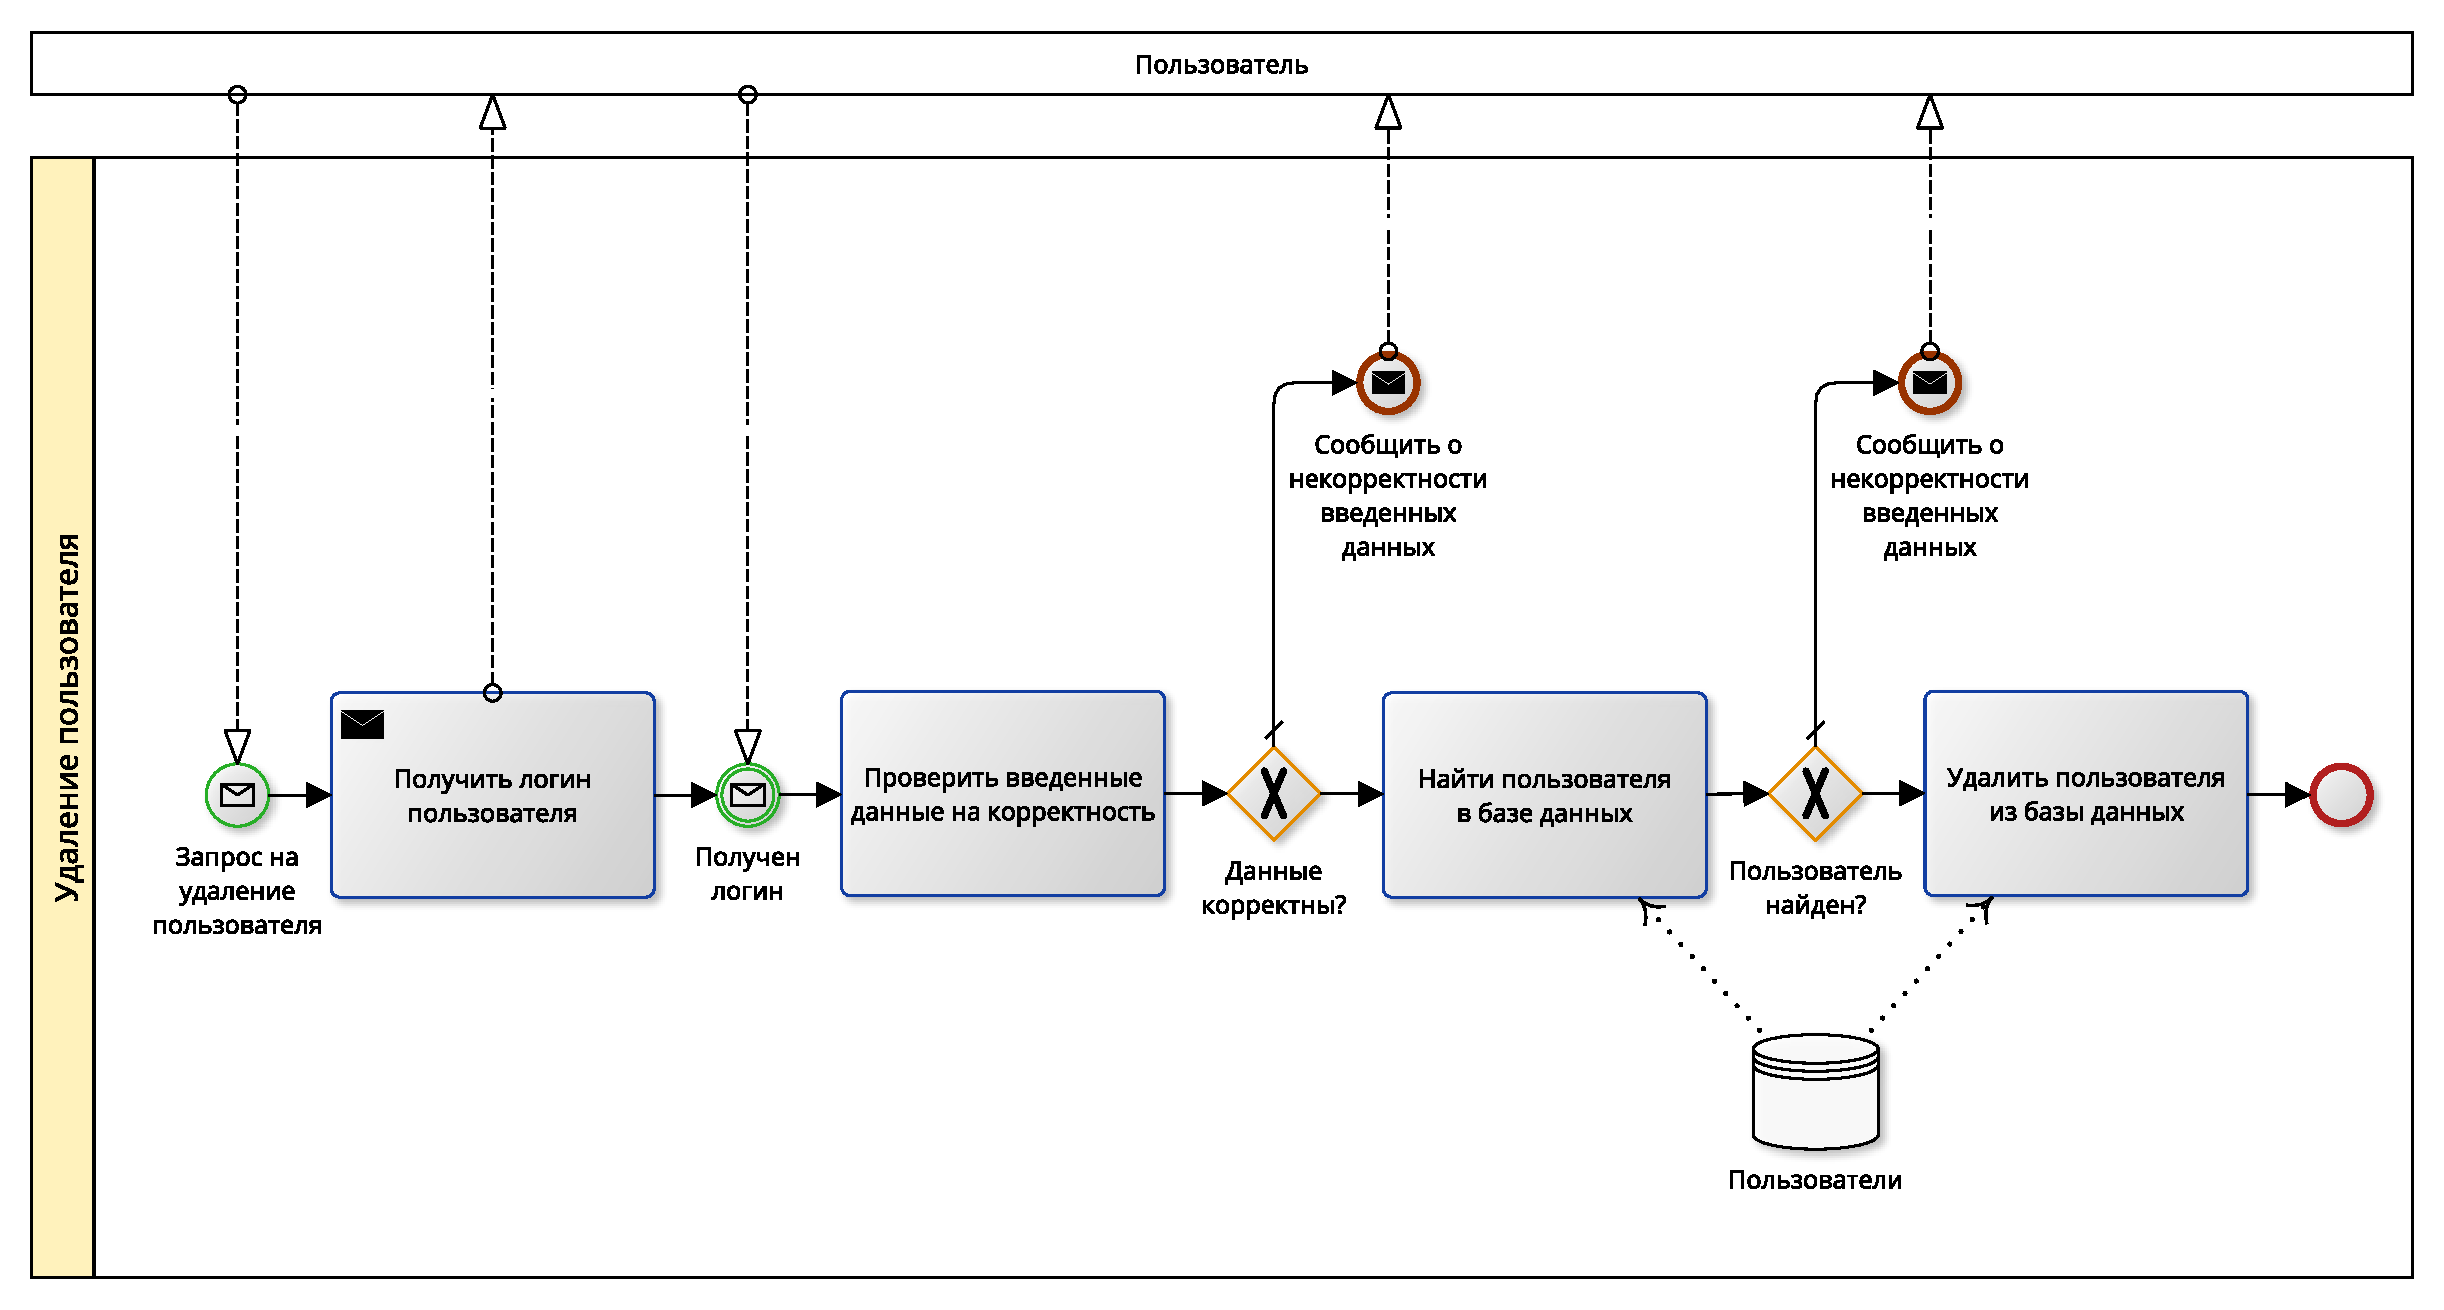
\includegraphics[width=\linewidth]{bpmn_removeuser}
	\caption{Бизнес-правило удаления пользователя}
	\label{bpmn_removeuser}
\end{figure}
\begin{figure}[H]
	\centering
	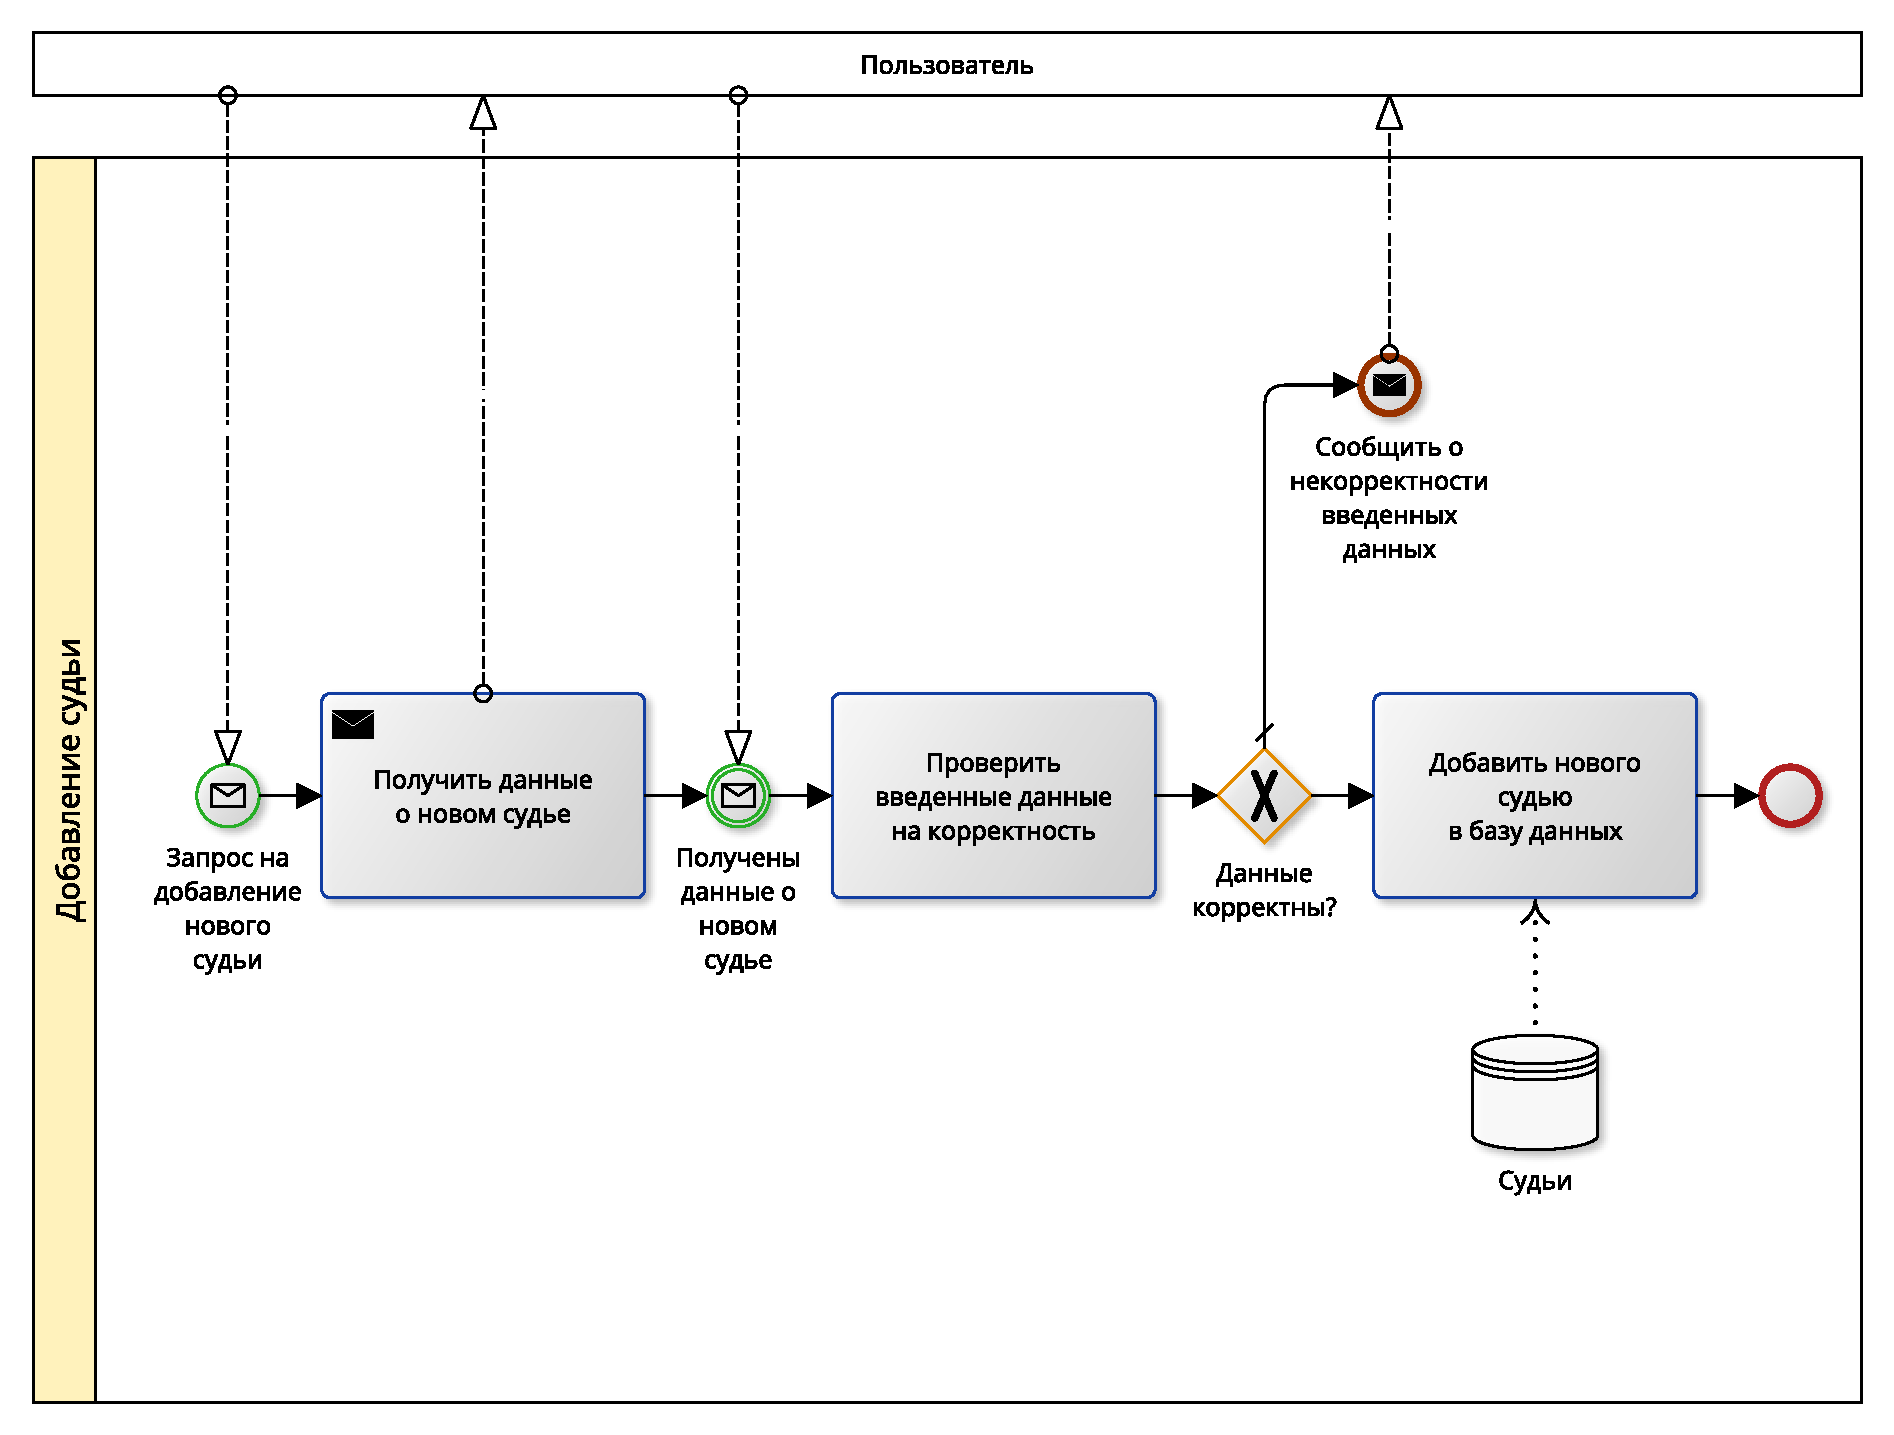
\includegraphics[width=\linewidth]{bpmn_addreferee}
	\caption{Бизнес-правило добавления судьи}
	\label{bpmn_addreferee}
\end{figure}
\begin{figure}[H]
	\centering
	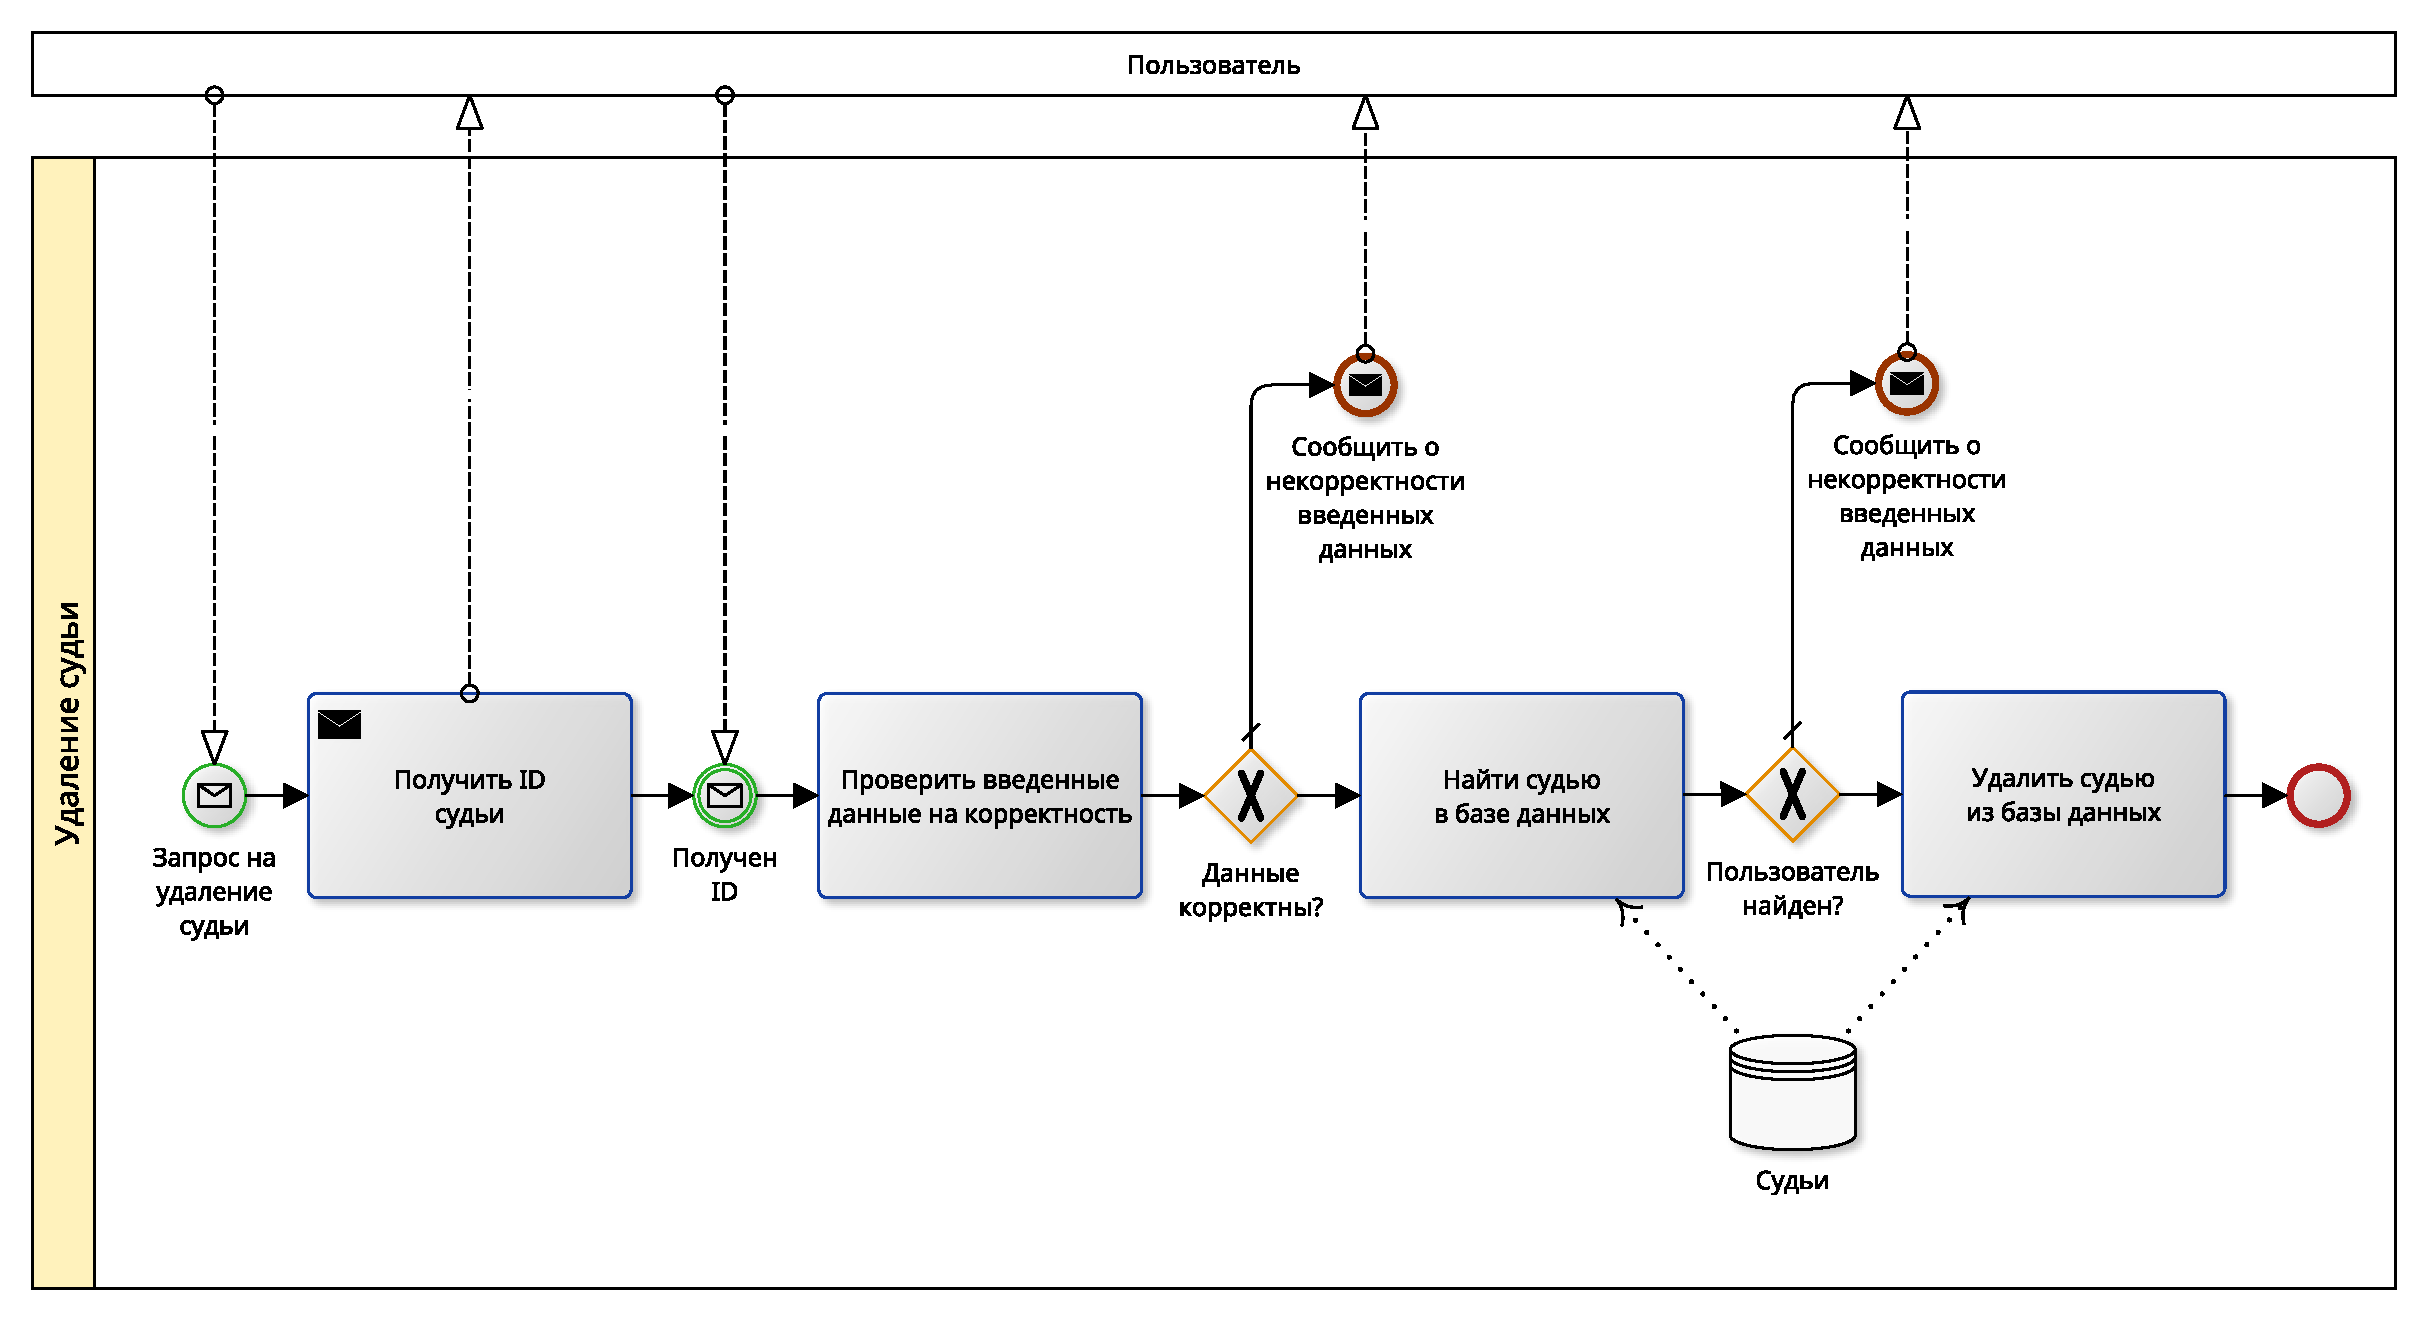
\includegraphics[width=\linewidth]{bpmn_removereferee}
	\caption{Бизнес-правило удаления судьи}
	\label{bpmn_removereferee}
\end{figure}

\section{Проектирование базы данных}

ER-диаграмма проектируемой базы данных представлена на рисунке~\ref{dber}.
\begin{figure}[H]
	\centering
	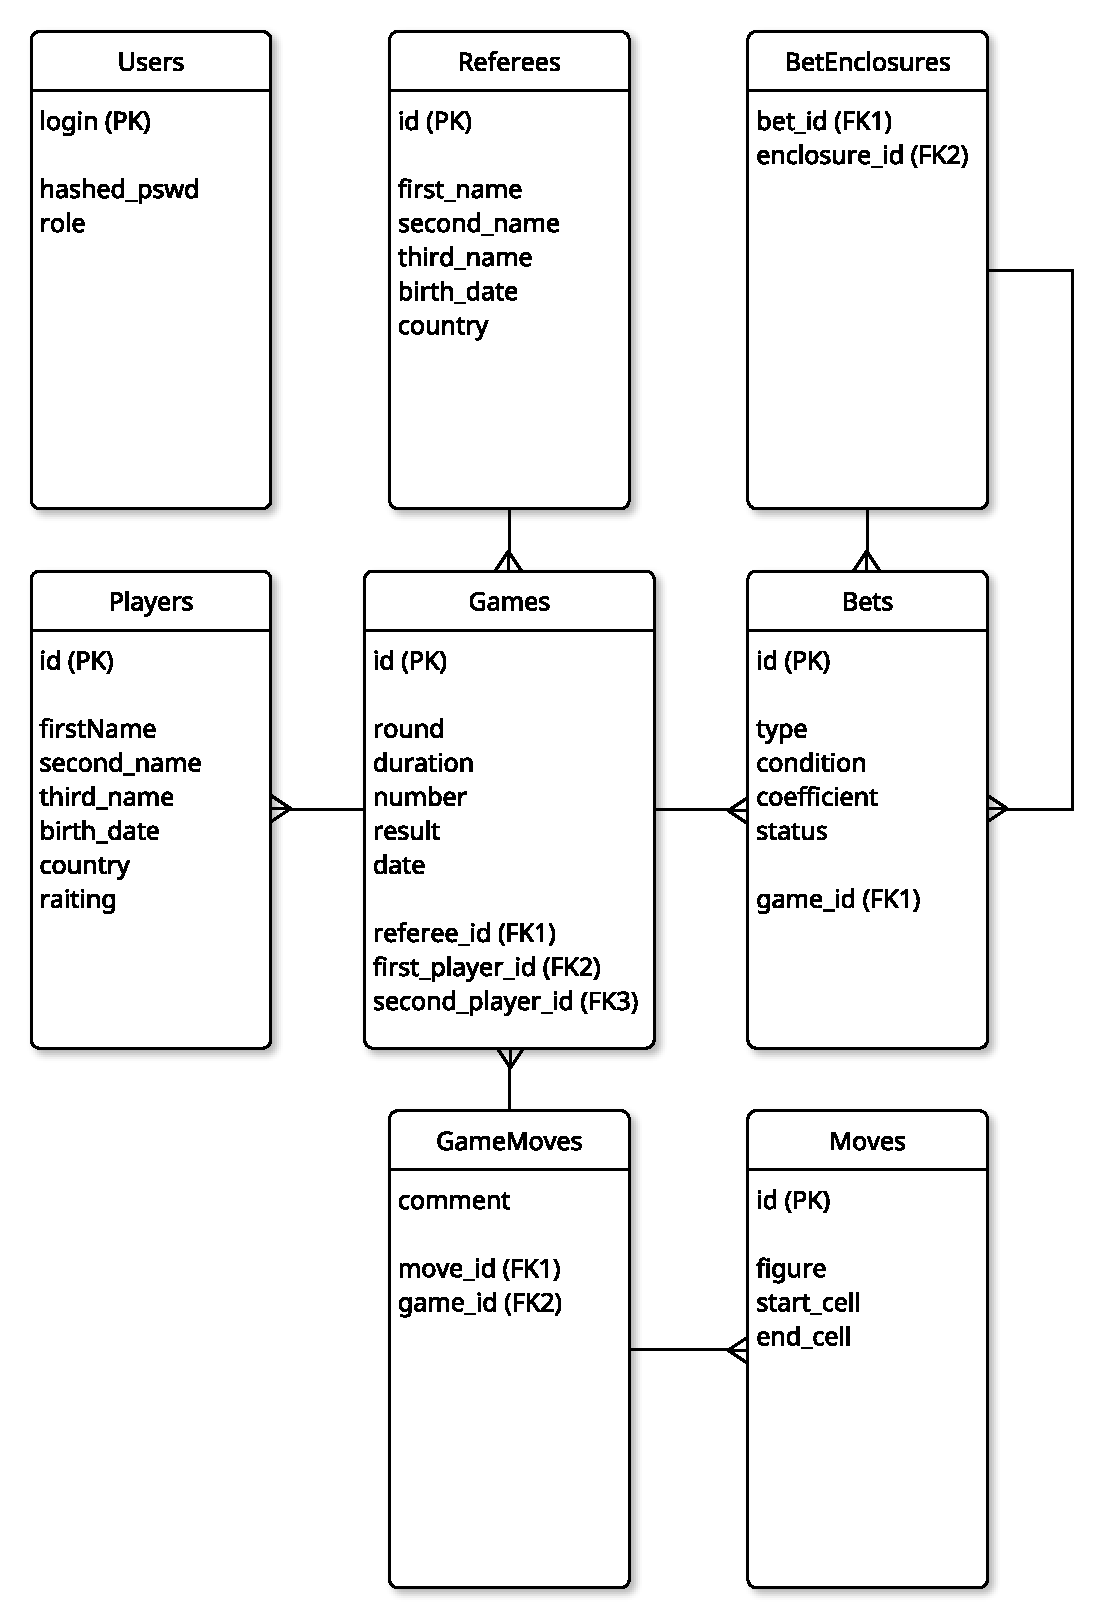
\includegraphics[width=0.6\linewidth]{dber}
	\caption{ER-диаграмма проектируемой базы данных}
	\label{dber}
\end{figure}

Проектируемая база данных содержит в себе следующие таблицы:
\begin{itemize}
	\item User~--- информация о пользователях системы;
	\item Game~--- информация о сыгранных шахматных партиях;
	\item Player~--- информация об игроках;
	\item Move~--- информация о ходах, сделанных в партиях;
	\item GameMoves~--- развязочная таблица для установления связи многие-ко-многим между шахматными партиями и ходами;
	\item Bet~--- информация о ставках;
	\item Referee~--- информация о судьях;
	\item BetEnclosures~--- развязочная таблица для описания вложенных ставок.
\end{itemize}

Описания полей таблиц базы данных представлены в таблицах~\ref{users_table}~--~\ref{gamemoves_table}.
\begin{center}
	\begin{threeparttable}
		\captionsetup{justification=raggedright,singlelinecheck=off}
		\caption{\label{users_table}Описание полей таблицы Users}
		\centering
		\begin{tabular}{|c|c|c|c|}
			\hline
			Название поля & Тип & Ограничения & Значение \\
			\hline
			login & Строка & \specialcell{Первичный ключ\\Не пустая строка} & Логин \\
			\hline
			hashed\_pswd & Строка & \specialcell{Не NULL\\Не пустая строка} & \specialcell{Хешированный\\пароль} \\
			\hline
			role & Целое число & \specialcell{Не NULL\\Значения:\\0~---~администратор\\1~---~наблюдатель\\2~---букмекер} & \specialcell{Роль\\пользователя} \\
			\hline
		\end{tabular}
	\end{threeparttable}
\end{center}
\begin{center}
	\begin{threeparttable}
		\captionsetup{justification=raggedright,singlelinecheck=off}
		\caption{\label{referees_table}Описание полей таблицы Referees}
		\centering
		\begin{tabular}{|c|c|c|c|}
			\hline
			Название поля & Тип & Ограничения & Значение \\
			\hline
			id & Целое число & Первичный ключ & Идентификатор \\
			\hline
			first\_name & Строка & \specialcell{Не NULL\\Не пустая строка} & Фамилия \\
			\hline
			second\_name & Строка & \specialcell{Не NULL\\Не пустая строка} & Имя \\
			\hline
			third\_name & Строка & --- & Отчество \\
			\hline
			birth\_date & Дата & Не NULL & Имя \\
			\hline
			country & Строка & \specialcell{Не NULL\\Не пустая строка} & Страна \\
			\hline
		\end{tabular}
	\end{threeparttable}
\end{center}
\begin{center}
	\begin{threeparttable}
		\captionsetup{justification=raggedright,singlelinecheck=off}
		\caption{\label{betenclosures_table}Описание полей таблицы BetEnclosures}
		\centering
		\begin{tabular}{|c|c|c|c|}
			\hline
			Название поля & Тип & Ограничения & Значение \\
			\hline
			bet\_id & Целое число & \specialcell{Вторичный ключ\\(поле id таблицы Bets)\\Не равен enclosure\_id} & \specialcell{Идентификатор\\ставки} \\
			\hline
			enclosure\_id & Целое число & \specialcell{Вторичный ключ\\(поле id таблицы Bets))\\Не равен bet\_id} & \specialcell{Идентификатор\\вложенной ставки} \\
			\hline
		\end{tabular}
	\end{threeparttable}
\end{center}
\begin{center}
	\begin{threeparttable}
		\captionsetup{justification=raggedright,singlelinecheck=off}
		\caption{\label{players_table}Описание полей таблицы Players}
		\centering
		\begin{tabular}{|c|c|c|c|}
			\hline
			Название поля & Тип & Ограничения & Значение \\
			\hline
			id & Целое число & Первичный ключ & Идентификатор \\
			\hline
			first\_name & Строка & \specialcell{Не NULL\\Не пустая строка} & Фамилия \\
			\hline
			second\_name & Строка & \specialcell{Не NULL\\Не пустая строка} & Имя \\
			\hline
			third\_name & Строка & --- & Отчество \\
			\hline
			birth\_date & Дата & Не NULL & Имя \\
			\hline
			country & Строка & \specialcell{Не NULL\\Не пустая строка} & Страна \\
			\hline
			raiting & Целое число & \specialcell{Не NULL\\Не отрицательное} & Рейтинг\\
			\hline
		\end{tabular}
	\end{threeparttable}
\end{center}
\begin{center}
	\begin{threeparttable}
		\captionsetup{justification=raggedright,singlelinecheck=off}
		\caption{\label{games_table}Описание полей таблицы Games}
		\centering
		\begin{tabular}{|c|c|c|c|}
			\hline
			Название поля & Тип & Ограничения & Значение \\
			\hline
			id & Целое число & Первичный ключ & Идентификатор \\
			\hline
			round & Целое число & \specialcell{Не NULL\\От 1 до 8} & Номер раунда \\
			\hline
			duration & Целое число & \specialcell{NULL или\\неотрицательное число} & \specialcell{Длительность партии\\в секундах} \\
			\hline
			number & Целое число & \specialcell{Не NULL\\Положительное} & \specialcell{Номер партии\\в раунде} \\
			\hline
			result & Целое число & \specialcell{NULL или\\одно из трех\\значений:\\0~---~ничья\\1~---~победа белых\\2~---победа черных} & Результат \\
			\hline
			date & Дата & --- & Дата проведения \\
			\hline
			referee\_id & Целое число & \specialcell{Вторичный ключ\\(поле id таблицы Referees)} & \specialcell{Идентификатор\\судьи}\\
			\hline
			first\_player\_id & Целое число & \specialcell{Вторичный ключ\\(поле id таблицы Players)\\Не равен second\_player\_id} & \specialcell{Идентификатор\\первого игрока}\\
			\hline
			second\_player\_id & Целое число & \specialcell{Вторичный ключ\\(поле id таблицы Players)\\Не равен first\_player\_id} & \specialcell{Идентификатор\\второго игрока}\\
			\hline
		\end{tabular}
	\end{threeparttable}
\end{center}
\begin{center}
	\begin{threeparttable}
		\captionsetup{justification=raggedright,singlelinecheck=off}
		\caption{\label{bets_table}Описание полей таблицы Bets}
		\centering
		\begin{tabular}{|c|c|c|c|}
			\hline
			Название поля & Тип & Ограничения & Значение \\
			\hline
			id & Целое число & Первичный ключ & Идентификатор \\
			\hline
			type & Целое число & \specialcell{Не NULL\\Значения:\\0~---~одинарная ставка\\1~---~экспресс\\2~---система} & \specialcell{Тип\\ставки} \\
			\hline
			condition & Строка & \specialcell{NULL или\\непустая строка} & \specialcell{Условие\\ставки}\\
			\hline
			coefficient & Вещественное число & \specialcell{NULL или число,\\ большее 1} & \specialcell{Коэффициенты\\ставки}\\
			\hline
			status & Целое число & \specialcell{Не NULL\\Значения:\\0~--- не известно,\\1~--- ставка сработала,\\2~--- ставка не сработала} & \specialcell{Статус\\ставки}\\
			\hline
			game\_id & Целое число & \specialcell{Вторичный ключ\\(поле id таблицы Games)} & \specialcell{Идентификатор\\шахматной партии}\\
			\hline
		\end{tabular}
	\end{threeparttable}
\end{center}
\begin{center}
	\begin{threeparttable}
		\captionsetup{justification=raggedright,singlelinecheck=off}
		\caption{\label{moves_table}Описание полей таблицы Moves}
		\centering
		\begin{tabular}{|c|c|c|c|}
			\hline
			Название поля & Тип & Ограничения & Значение \\
			\hline
			id & Целое число & Первичный ключ & Идентификатор \\
			\hline
			figure & Целое число & \specialcell{Не NULL\\Значения:\\0~---~король\\1~---~ферзь\\2~---~ладья\\3~---~слон\\4~---~конь\\5~---~пешка} & Фигура\\
			\hline
			start\_cell & Строка & \specialcell{Не NULL\\Не пустая строка} & \specialcell{Начальная\\клетка} \\
			\hline
			end\_cell & Строка & \specialcell{Не NULL\\Не пустая строка} & \specialcell{Конечная\\клетка} \\
			\hline
		\end{tabular}
	\end{threeparttable}
\end{center}
\begin{center}
	\begin{threeparttable}
		\captionsetup{justification=raggedright,singlelinecheck=off}
		\caption{\label{gamemoves_table}Описание полей таблицы GameMoves}
		\centering
		\begin{tabular}{|c|c|c|c|}
			\hline
			Название поля & Тип & Ограничения & Значение \\
			\hline
			move\_id & Целое число & \specialcell{Вторичный ключ\\(поле id таблицы Moves)} & \specialcell{Идентификатор\\хода} \\
			\hline
			game\_id & Целое число & \specialcell{Вторичный ключ\\(поле id таблицы Games)} & \specialcell{Идентификатор\\шахматной партии} \\
			\hline
			number & Целое число & \specialcell{Не NULL\\Положительное} & Номер хода \\
			\hline
			comment & Строка & --- & Комментарий \\
			\hline
		\end{tabular}
	\end{threeparttable}
\end{center}

\section{Ролевая модель проектируемой базы данных}

В аналитической части были выделены следующие роли:
\begin{itemize}
	\item неавторизованный пользователь,
	\item администратор,
	\item наблюдатель,
	\item букмекер.
\end{itemize}

В таблицах~\ref{unauth_privileges}~--~\ref{bookmaker_privileges} приведена информация о доступе ролей к объектам проектируемой базы данных.
\begin{center}
	\begin{threeparttable}
		\captionsetup{justification=raggedright,singlelinecheck=off}
		\caption{\label{unauth_privileges}Доступ неавторизованного пользователя к объектам базы данных}
		\centering
		\begin{tabular}{|c|c|c|c|c|c|c|c|c|}
			\hline
			& \multicolumn{8}{|c|}{Таблица} \\
			\hline
			Разрешения & Users & Referees & Players & Games & Bets & Moves & Bet & Game \\
			&&&&&&& Enclosures & Moves \\
			\hline
			Select & + & - & - & - & - & - & - & - \\
			\hline
			Insert & - & - & - & - & - & - & - & - \\
			\hline
			Update & - & - & - & - & - & - & - & - \\
			\hline
			Delete & - & - & - & - & - & - & - & - \\
			\hline
		\end{tabular}
	\end{threeparttable}
\end{center}
\begin{center}
	\begin{threeparttable}
		\captionsetup{justification=raggedright,singlelinecheck=off}
		\caption{\label{admin_privileges}Доступ администратора к объектам базы данных}
		\centering
		\begin{tabular}{|c|c|c|c|c|c|c|c|c|}
			\hline
			& \multicolumn{8}{|c|}{Таблица} \\
			\hline
			Разрешения & Users & Referees & Players & Games & Bets & Moves & Bet & Game \\
			&&&&&&& Enclosures & Moves \\
			\hline
			Select & + & + & + & + & + & + & + & + \\
			\hline
			Insert& + & + & + & + & + & + & + & + \\
			\hline
			Update & + & + & + & + & + & + & + & + \\
			\hline
			Delete & + & + & + & + & + & + & + & + \\
			\hline
		\end{tabular}
	\end{threeparttable}
\end{center}
\begin{center}
	\begin{threeparttable}
		\captionsetup{justification=raggedright,singlelinecheck=off}
		\caption{\label{spectator_privileges}Доступ наблюдателя к объектам базы данных}
		\centering
		\begin{tabular}{|c|c|c|c|c|c|c|c|c|}
			\hline
			& \multicolumn{8}{|c|}{Таблица} \\
			\hline
			Разрешения & Users & Referees & Players & Games & Bets & Moves & Bet & Game \\
			&&&&&&& Enclosures & Moves \\
			\hline
			Select & - & + & + & + & - & + & - & + \\
			\hline
			Insert & - & - & - & + & - & + & - & + \\
			\hline
			Update & - & - & - & + & - & + & - & + \\
			\hline
			Delete & - & - & - & + & - & + & - & + \\
			\hline
		\end{tabular}
	\end{threeparttable}
\end{center}
\begin{center}
	\begin{threeparttable}
		\captionsetup{justification=raggedright,singlelinecheck=off}
		\caption{\label{bookmaker_privileges}Доступ букмекера к объектам базы данных}
		\centering
		\begin{tabular}{|c|c|c|c|c|c|c|c|c|}
			\hline
			& \multicolumn{8}{|c|}{Таблица} \\
			\hline
			Разрешения & Users & Referees & Players & Games & Bets & Moves & Bet & Game \\
			&&&&&&& Enclosures & Moves \\
			\hline
			Select & - & + & + & + & + & + & + & + \\
			\hline
			Insert & - & - & - & - & + & - & + & - \\
			\hline
			Update & - & - & - & - & + & - & + & - \\
			\hline
			Delete & - & - & - & - & + & - & + & - \\
			\hline
		\end{tabular}
	\end{threeparttable}
\end{center}

\section{Триггеры}

Для корректной работы с данными необходимо реализовать следующие триггеры:
\begin{itemize}
	\item проверка на выполнение условий ставок (главной линии, экспрессов, содержащих только главные линии; систем, содержащих экспрессы с главными линиями) после добавления завершенной партии в базу данных;
	\item обновление рейтинга игроков после завершения партии в базу данных;
	\item удаление ходов из партии.
\end{itemize}

Схема алгоритма триггера проверки на выполнение условий ставок приведена на рисунке~\ref{raiting_trigger_flowchart}.
Схема алгоритма триггера обновления рейтинга игроков представлен на рисунках~\ref{bet_check_trigger1}~--~\ref{express_is_activated}.
Схема алгоритма удаления ходов из шахматной партии приведен на рисунках~\ref{delete_moves_trigger_flowchart}~и~\ref{delete_free_moves}.
\begin{figure}[H]
	\centering
	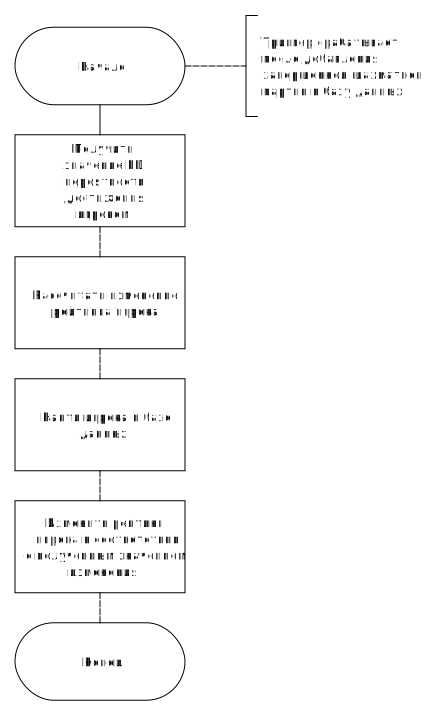
\includegraphics[width=0.4\linewidth]{raiting_trigger}
	\caption{Схема алгоритма триггера проверки на выполнение условий ставок}
	\label{raiting_trigger_flowchart}
\end{figure}
\begin{figure}[H]
	\centering
	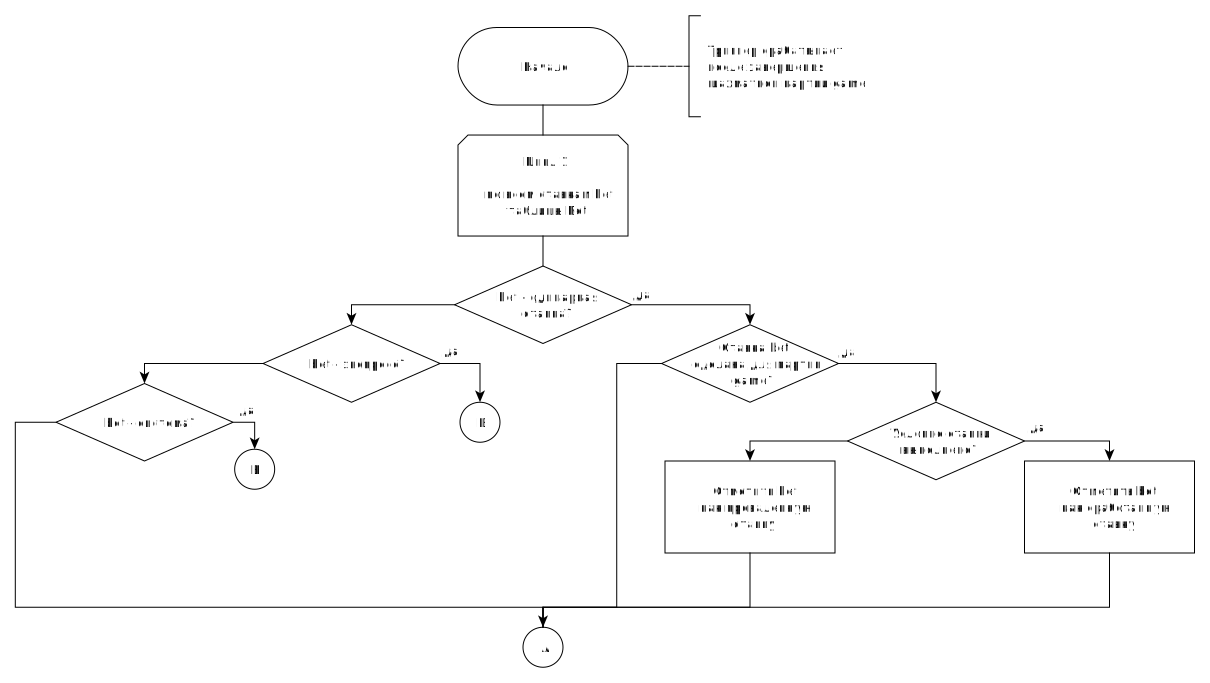
\includegraphics[width=0.8\linewidth]{bet_check_trigger1}
	\caption{Схема алгоритма триггера обновления рейтинга игроков (начало)}
	\label{bet_check_trigger1}
\end{figure}
\begin{figure}[H]
	\centering
	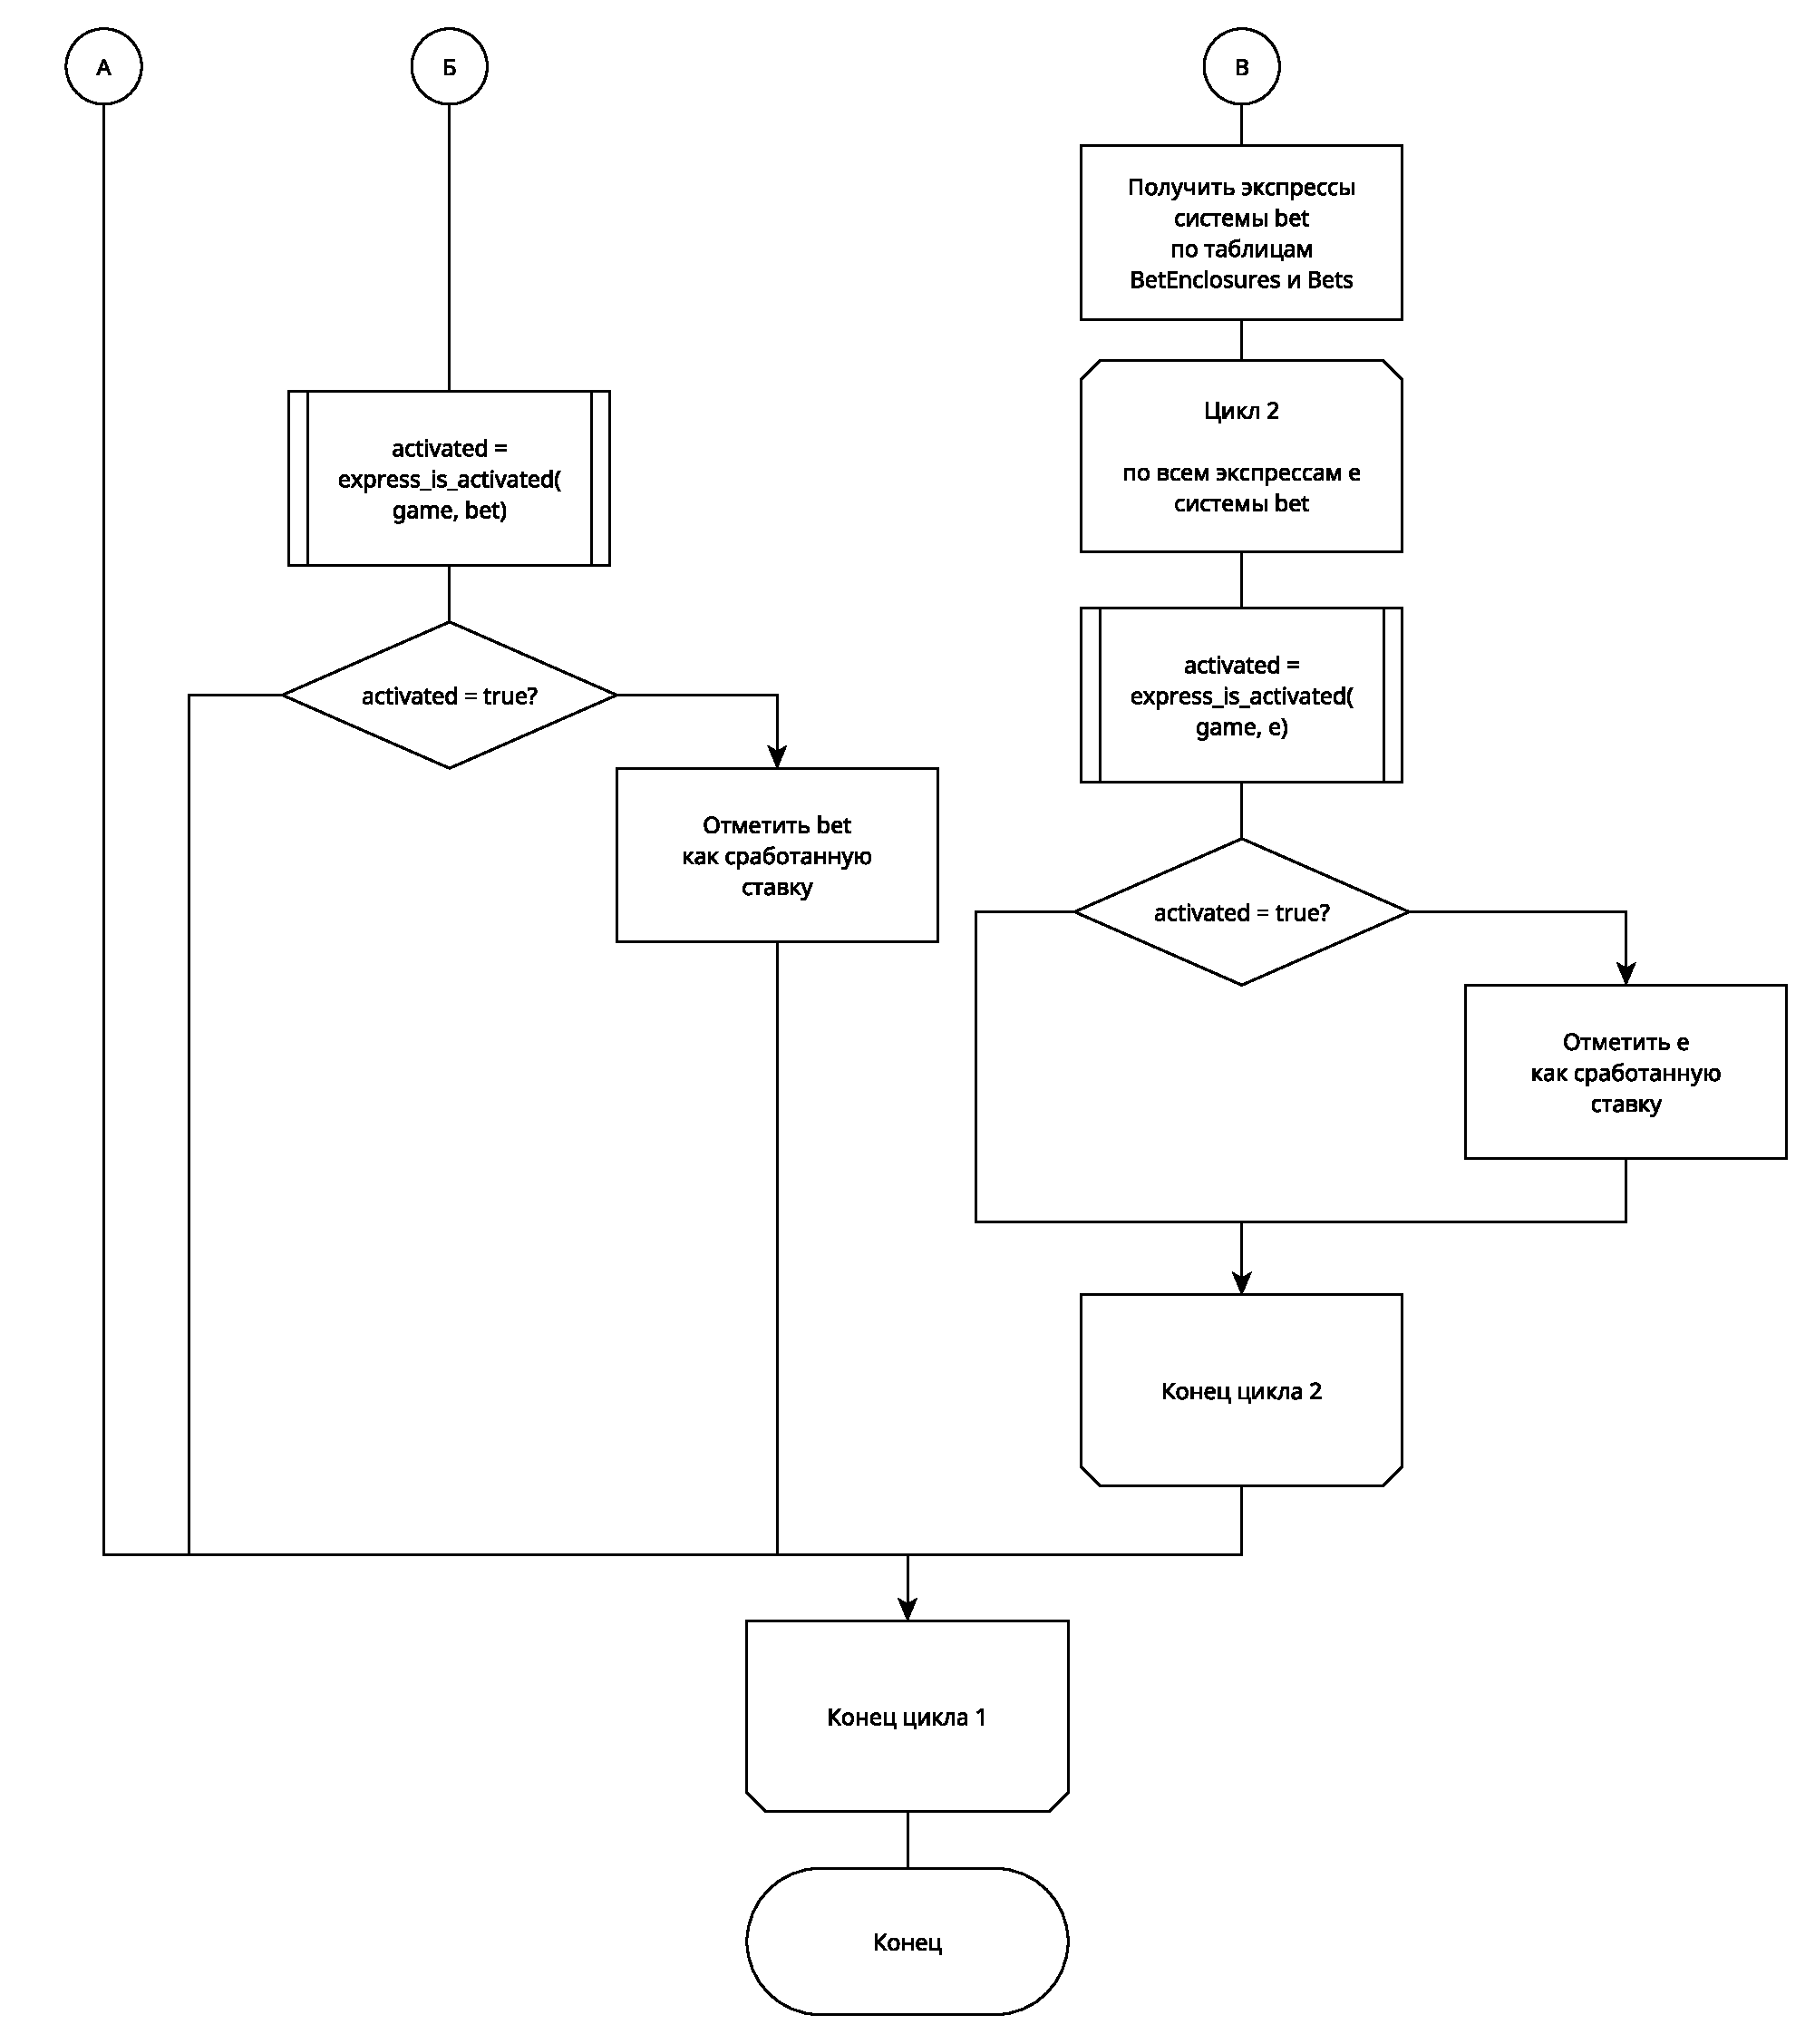
\includegraphics[width=0.5\linewidth]{bet_check_trigger2}
	\caption{Схема алгоритма триггера обновления рейтинга игроков (конец)}
	\label{bet_check_trigger2}
\end{figure}
\begin{figure}[H]
	\centering
	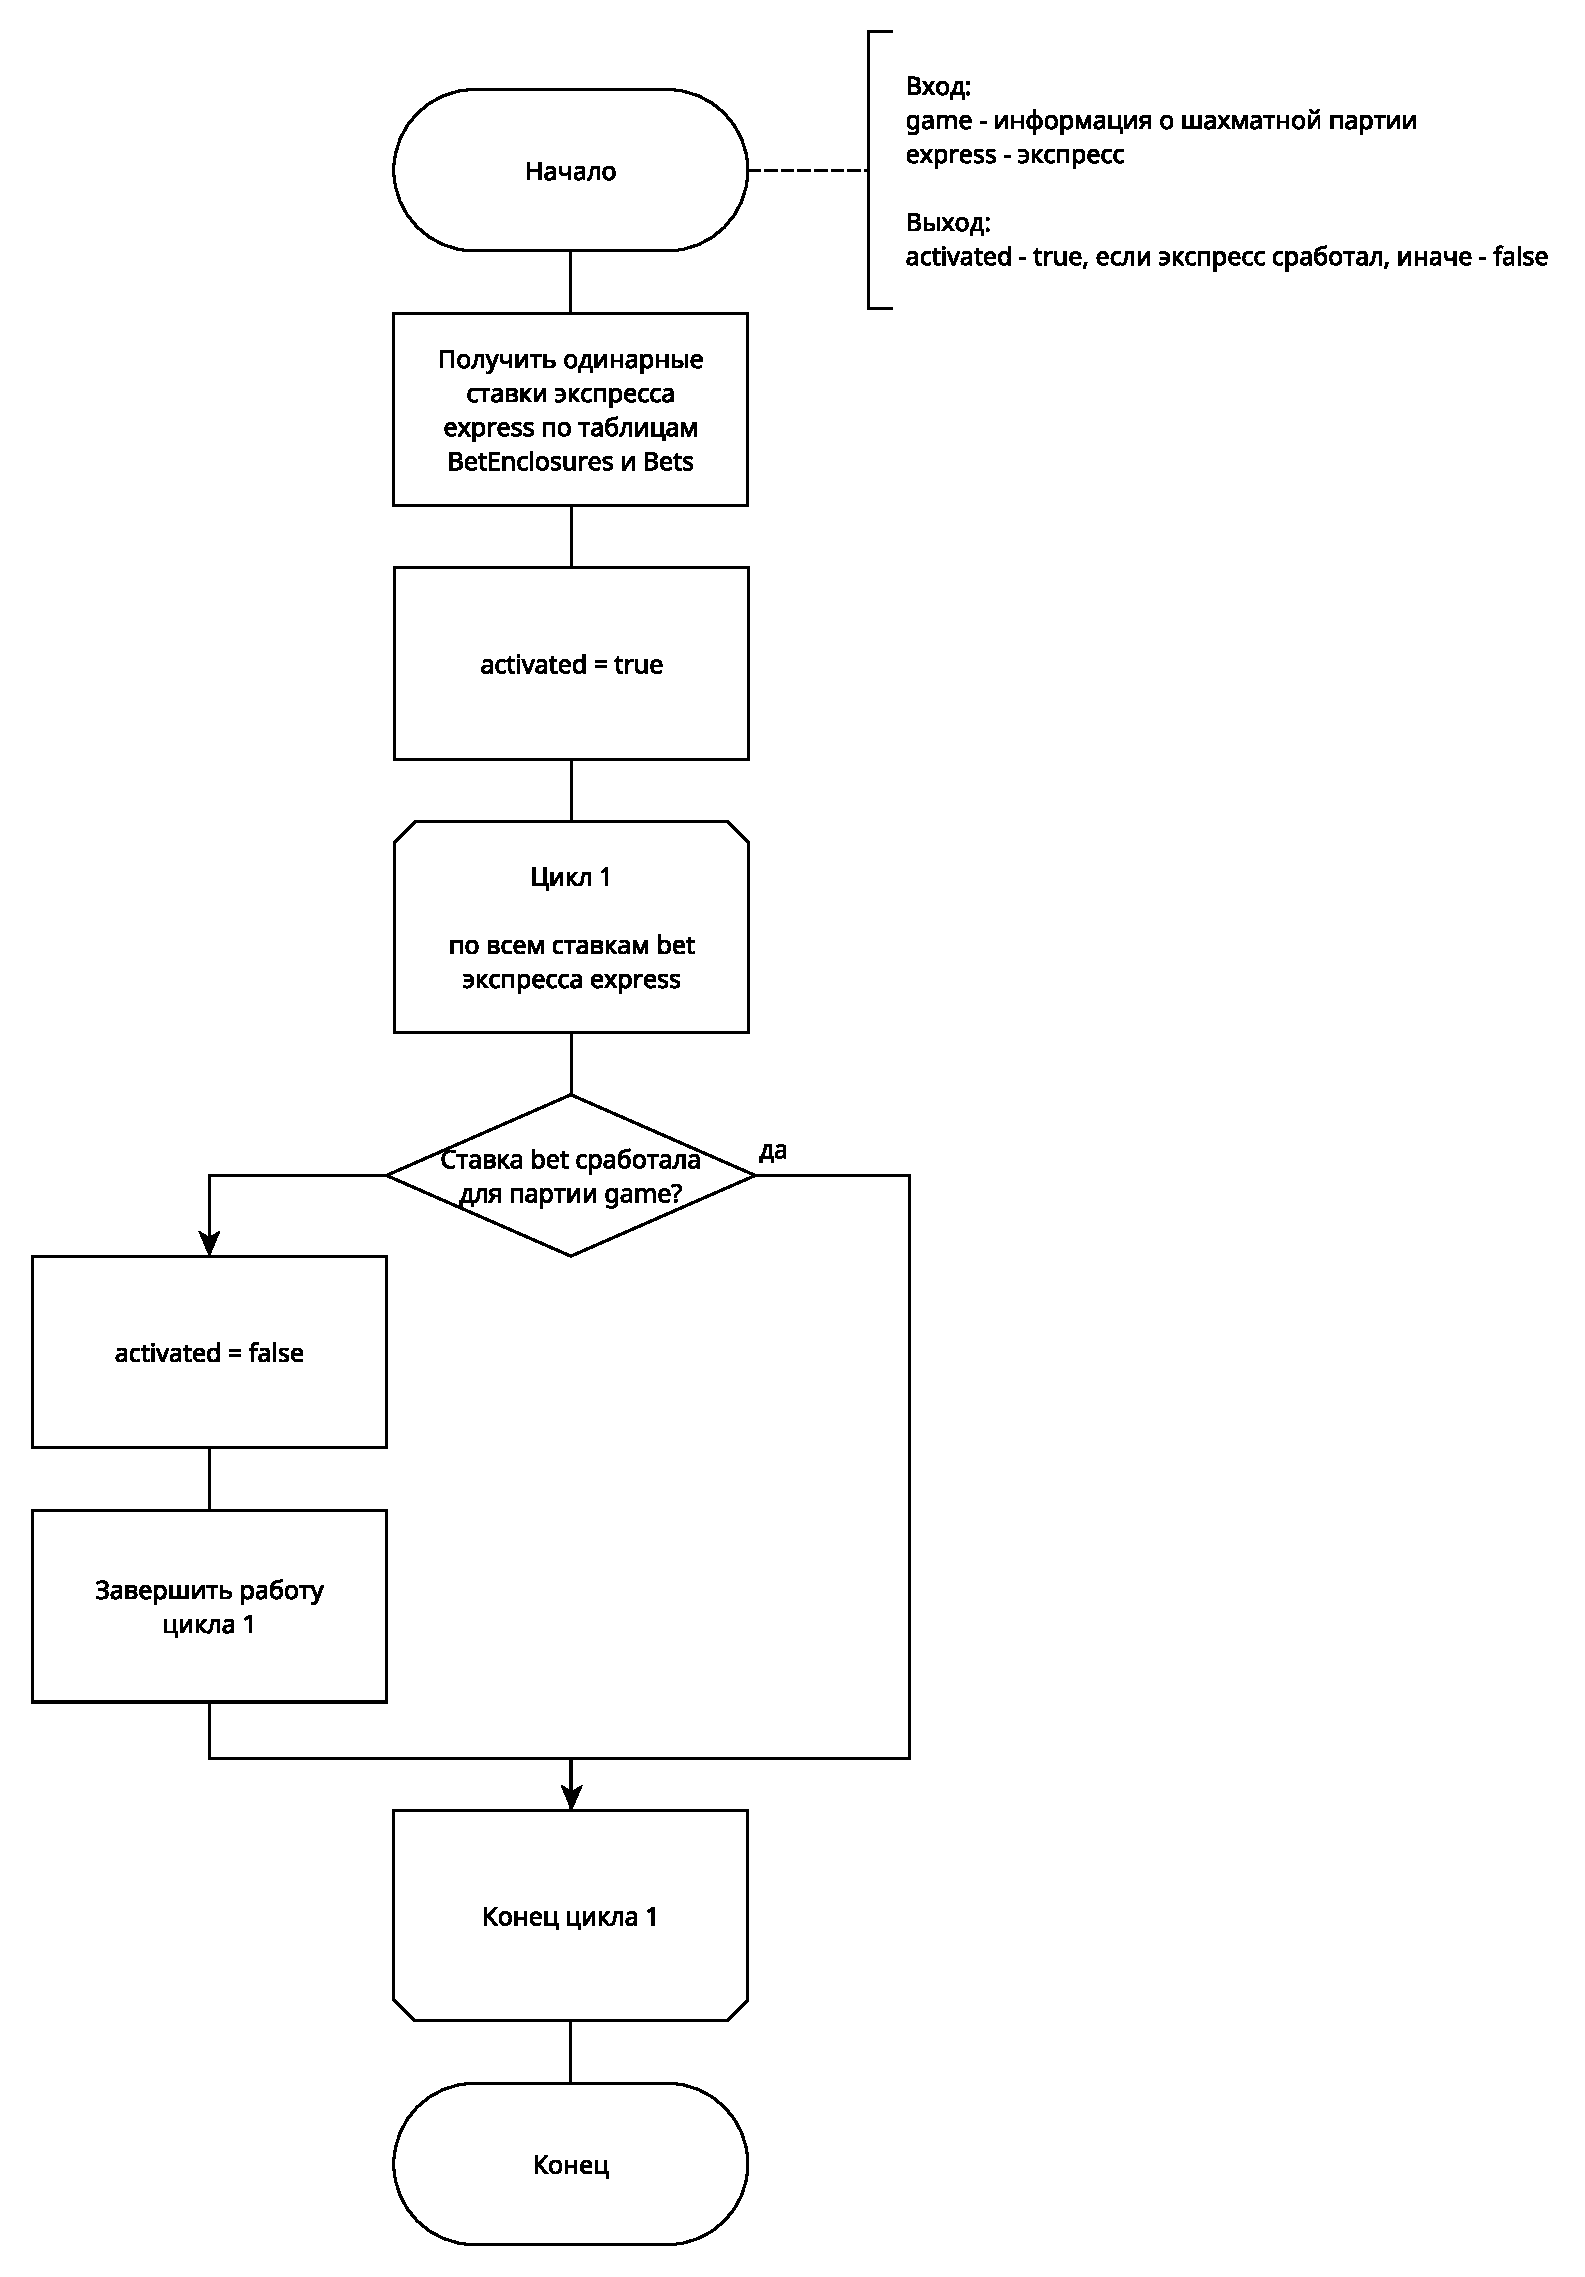
\includegraphics[width=0.5\linewidth]{express_is_activated}
	\caption{Схема алгоритма функции express\_is\_activated}
	\label{express_is_activated}
\end{figure}
\begin{figure}[H]
	\centering
	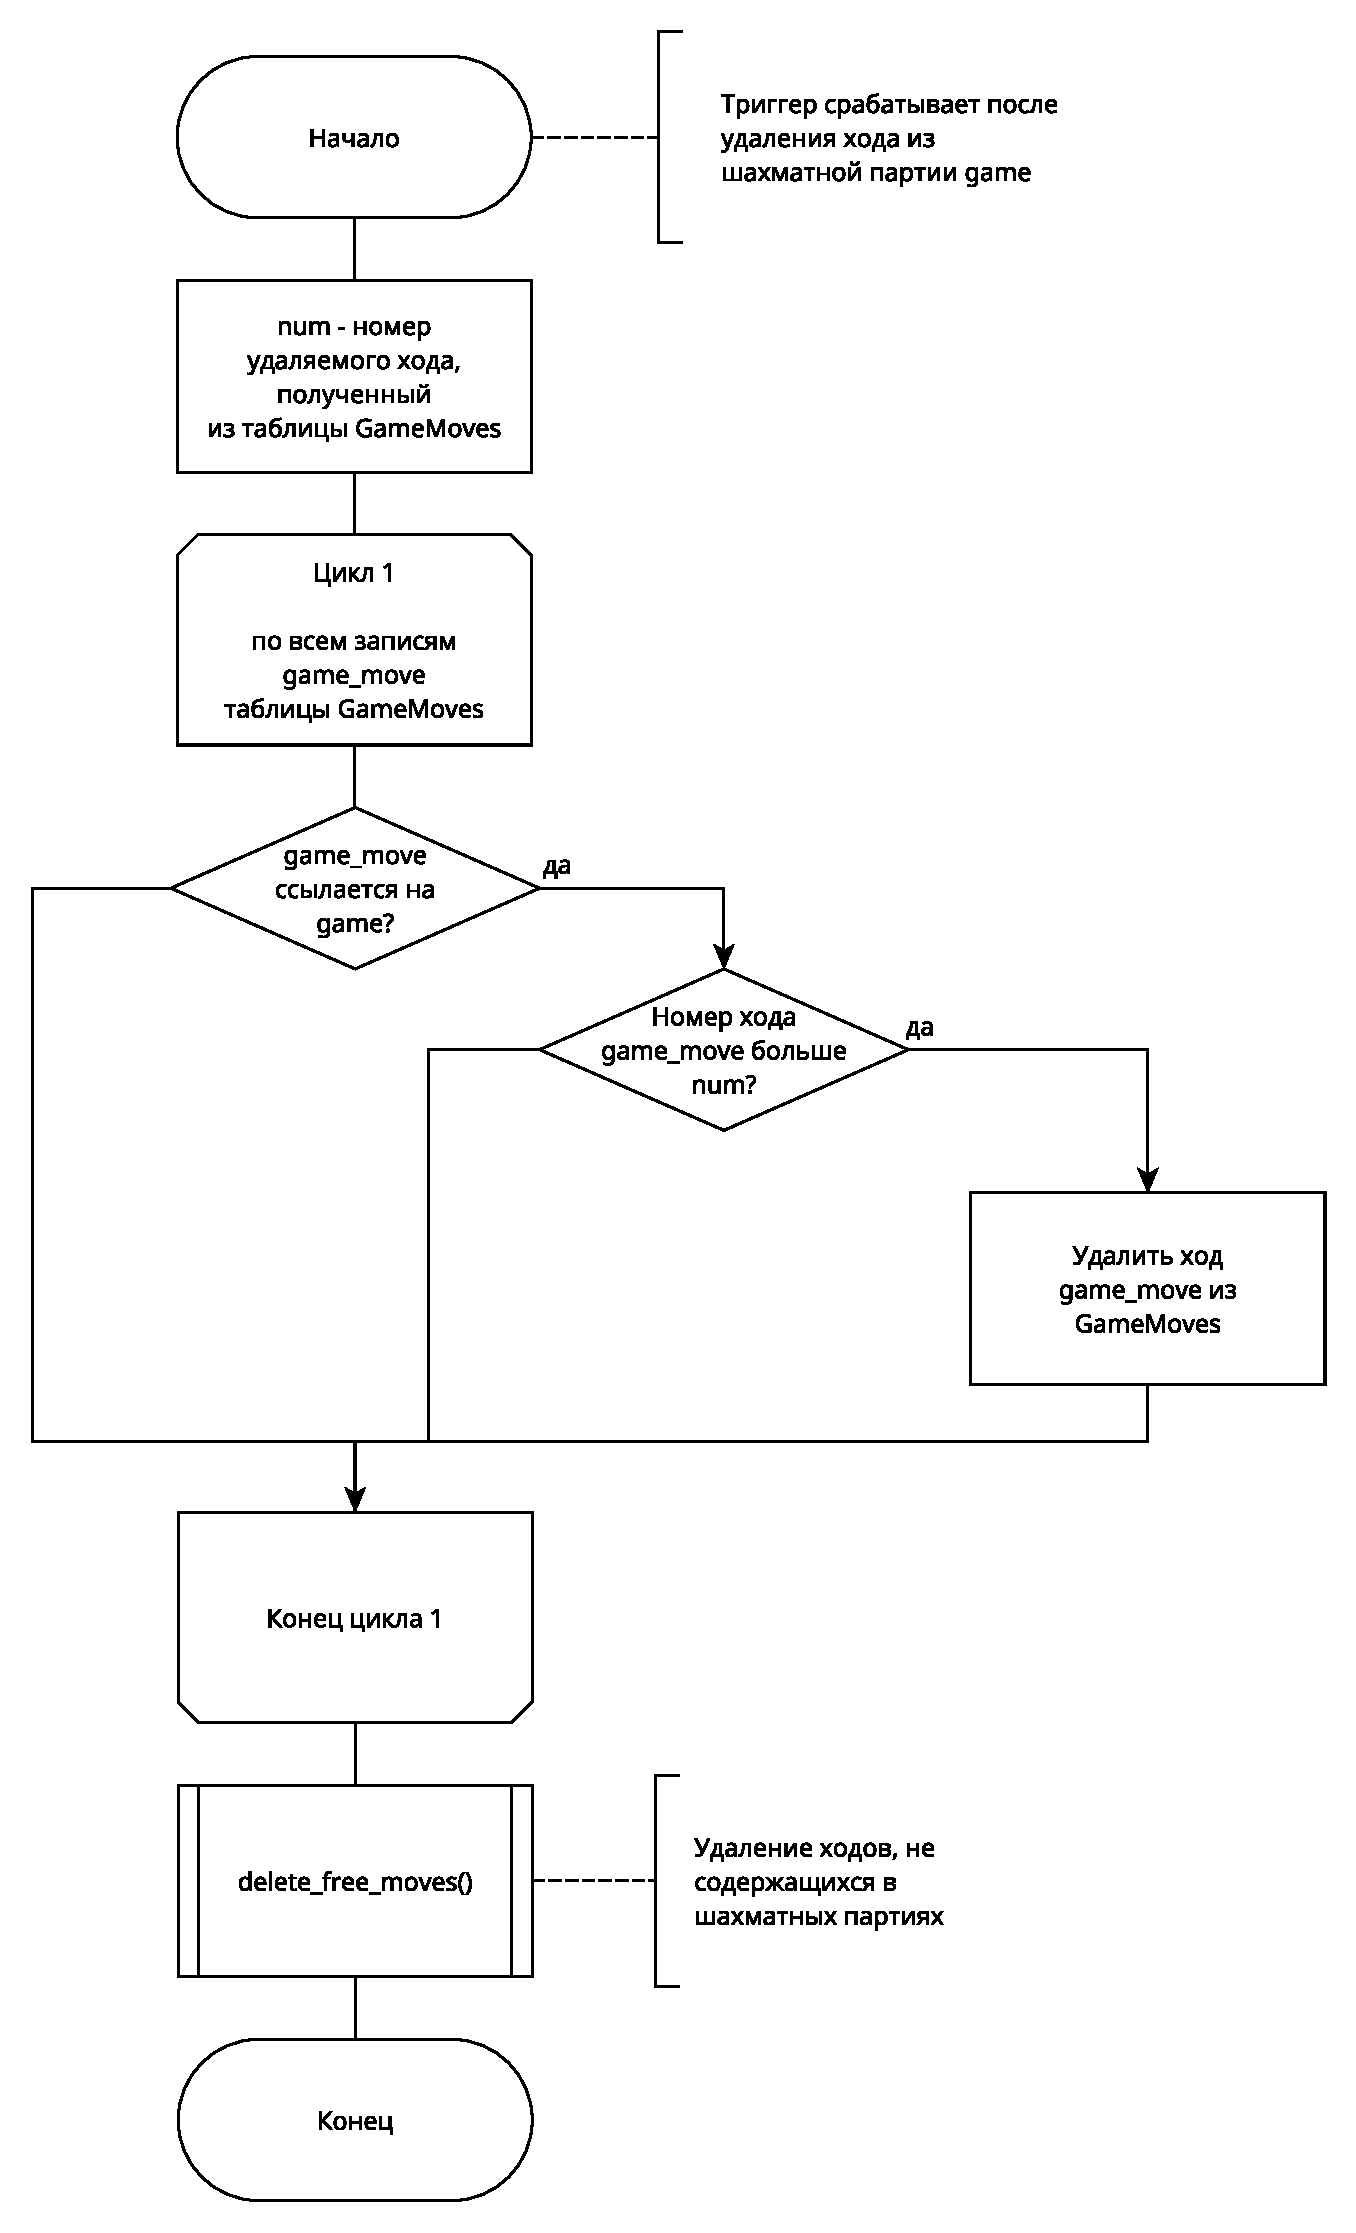
\includegraphics[width=0.5\linewidth]{delete_moves_trigger}
	\caption{Схема алгоритма удаления ходов из шахматной партии}
	\label{delete_moves_trigger_flowchart}
\end{figure}
\begin{figure}[H]
	\centering
	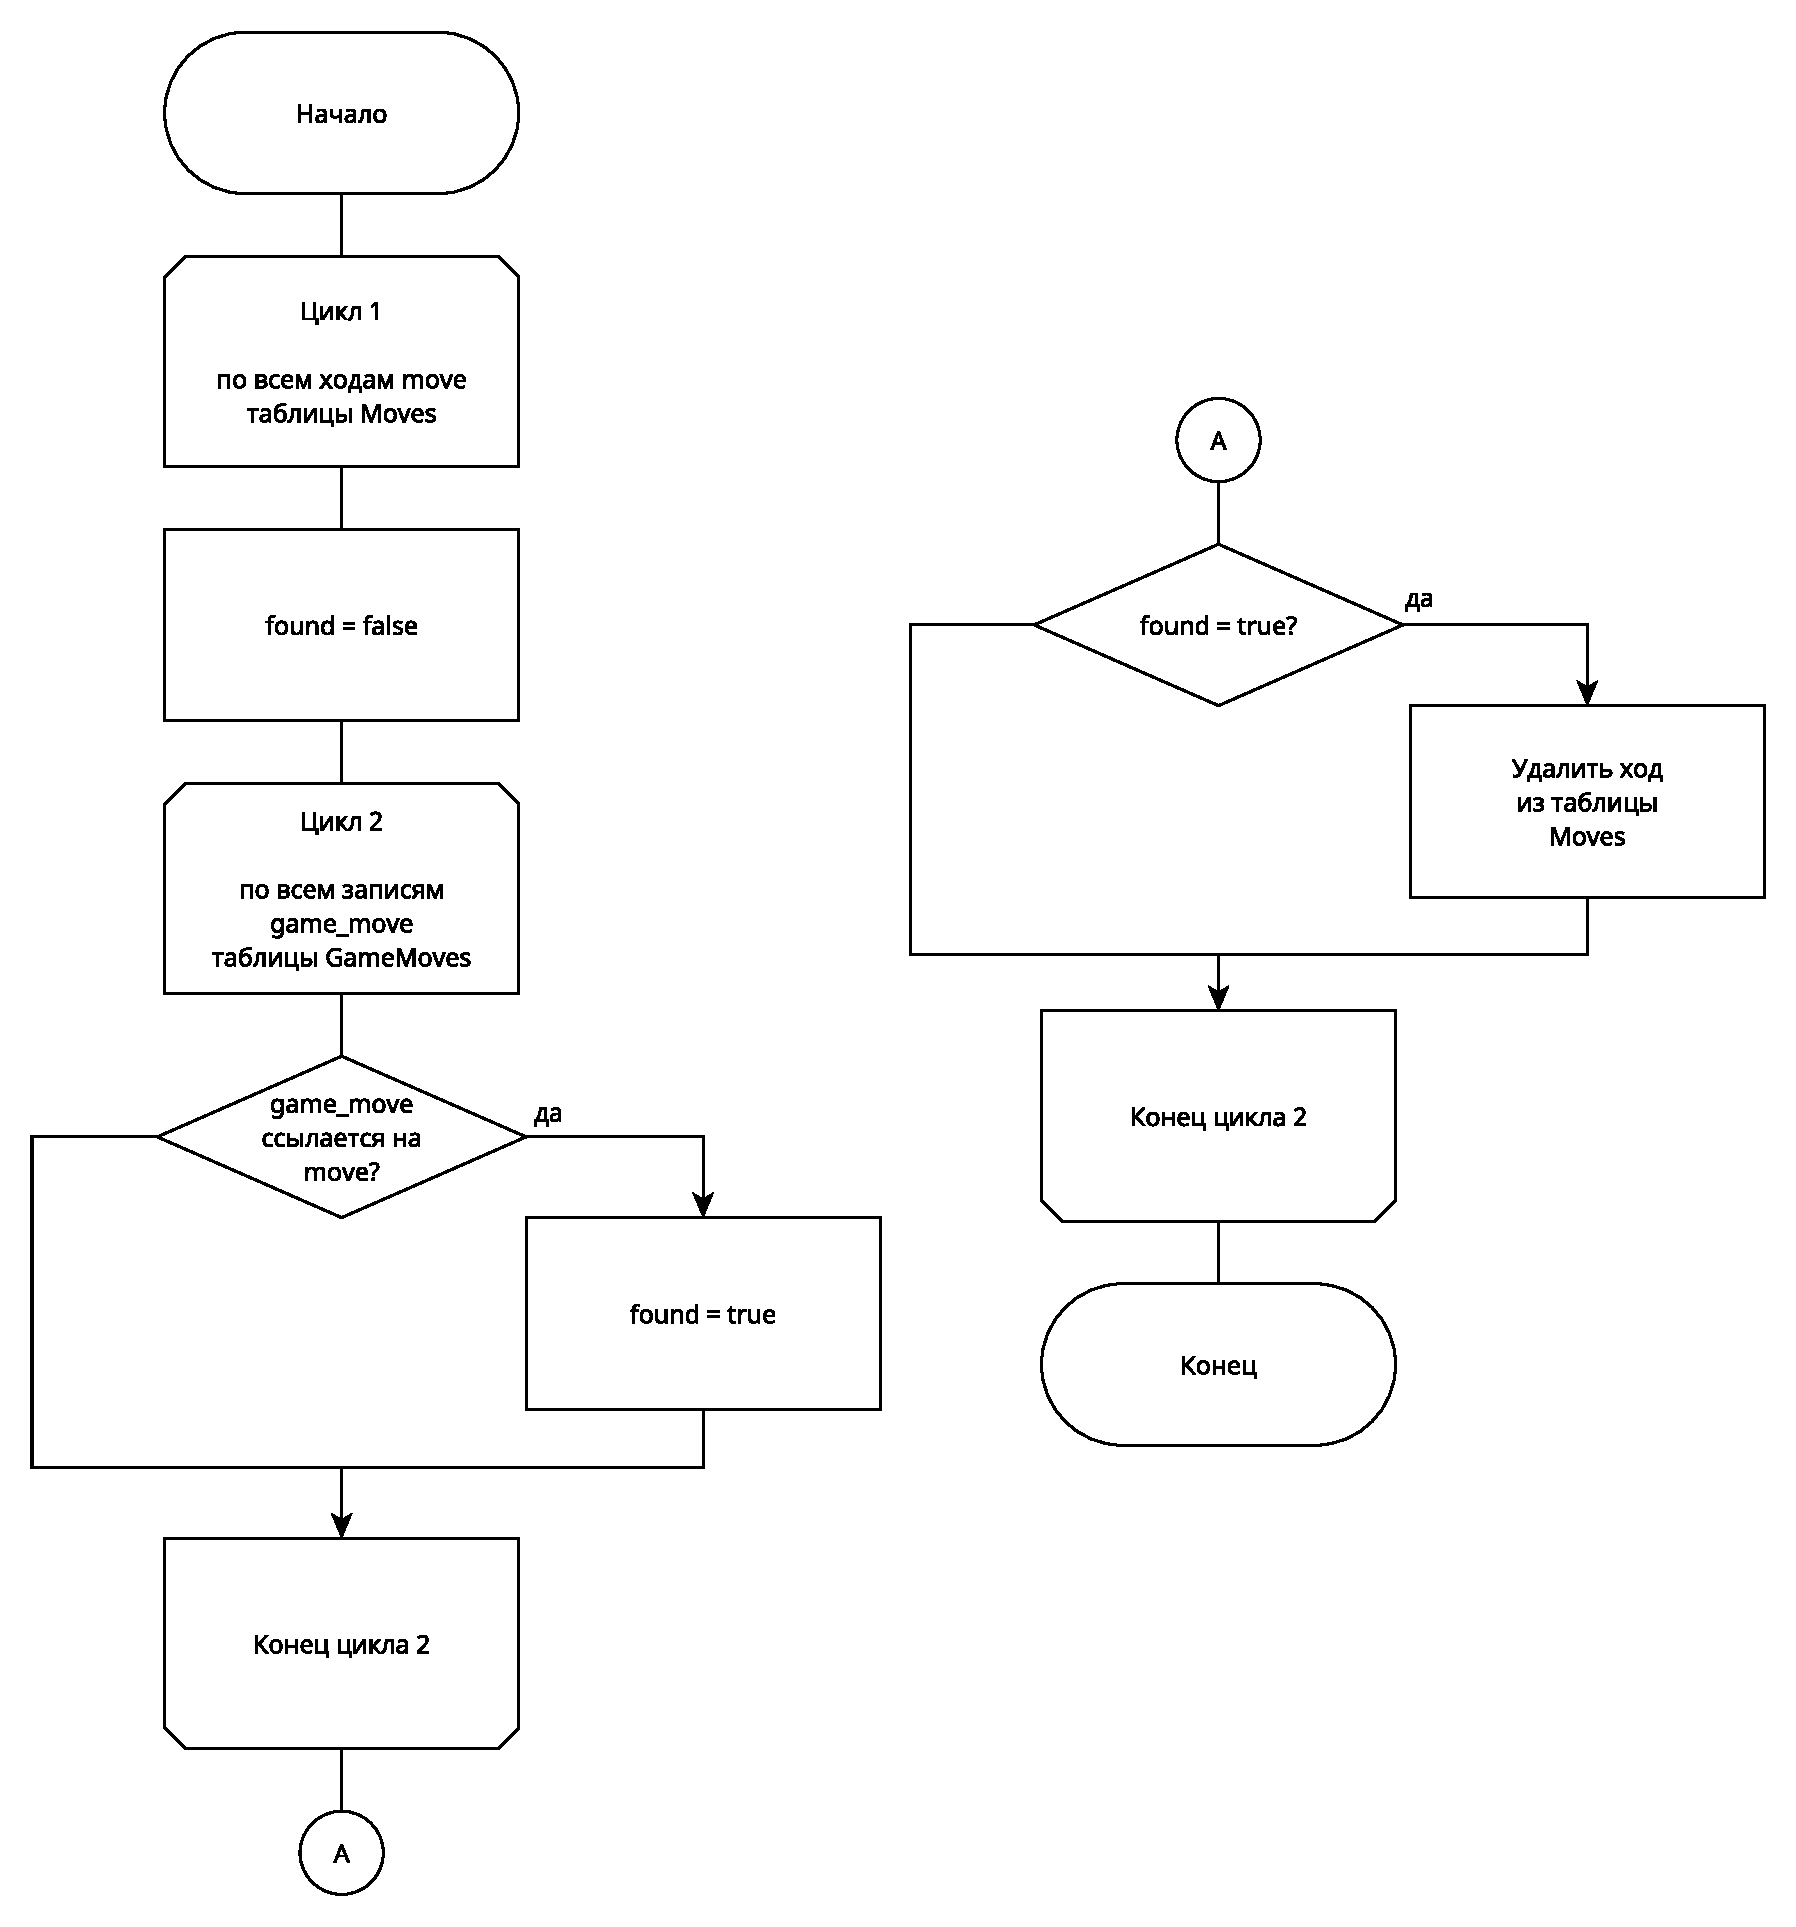
\includegraphics[width=0.5\linewidth]{delete_free_moves}
	\caption{Схема алгоритма функции delete\_free\_moves}
	\label{delete_free_moves}
\end{figure}

На рисунках~\ref{raiting_trigger_seq_diag}~--~\ref{bet_check_trigger_seq_diag} приведены диаграммы последовательности работы триггеров.
\begin{figure}[H]
	\centering
	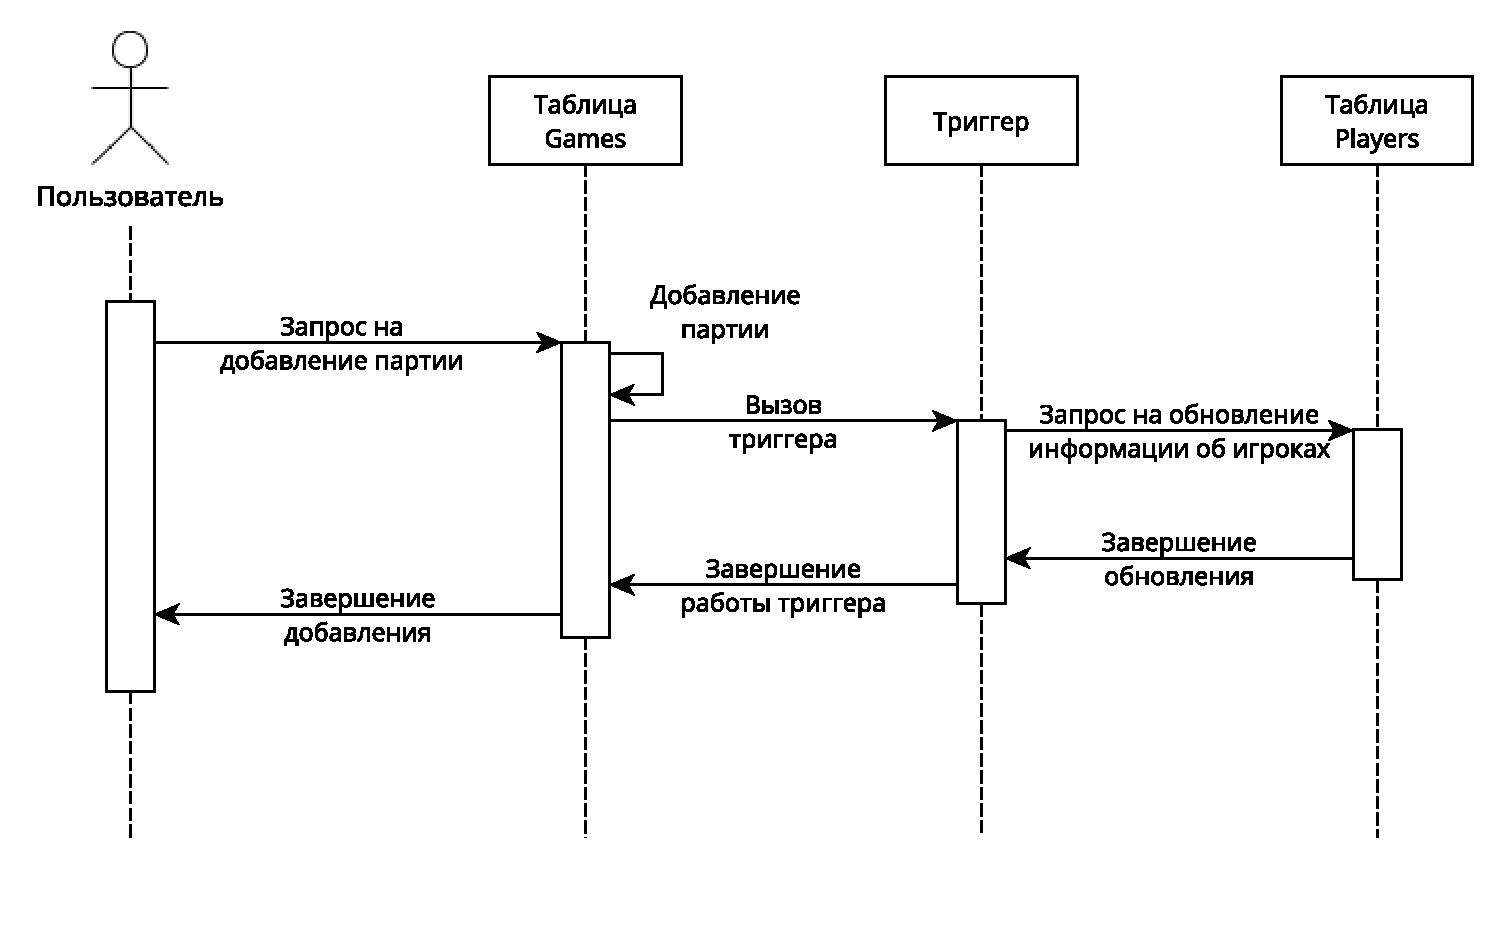
\includegraphics[width=0.7\linewidth]{raiting_trigger_seq_diag}
	\caption{Диаграмма последовательности триггера обновления рейтинга игроков}
	\label{raiting_trigger_seq_diag}
\end{figure}
\begin{figure}[H]
	\centering
	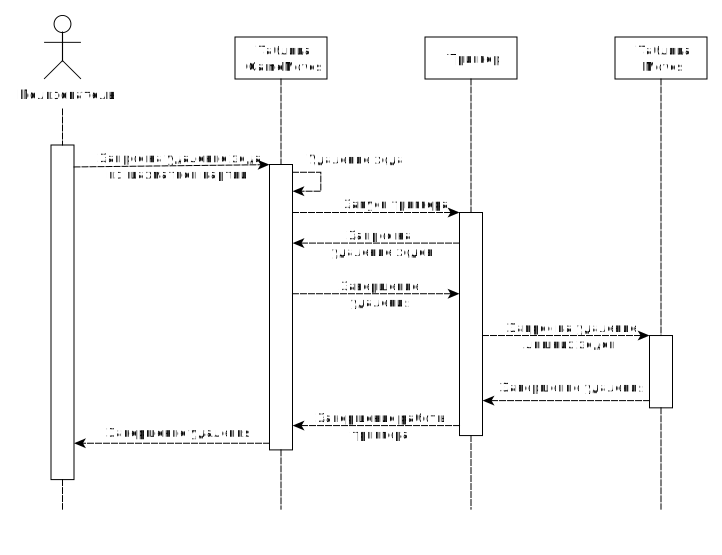
\includegraphics[width=0.7\linewidth]{delete_moves_trigger_seq_diag}
	\caption{Диаграмма последовательности триггера удаления ходов из шахматной партии}
	\label{delete_moves_trigger_seq_diag}
\end{figure}
\begin{figure}[H]
	\centering
	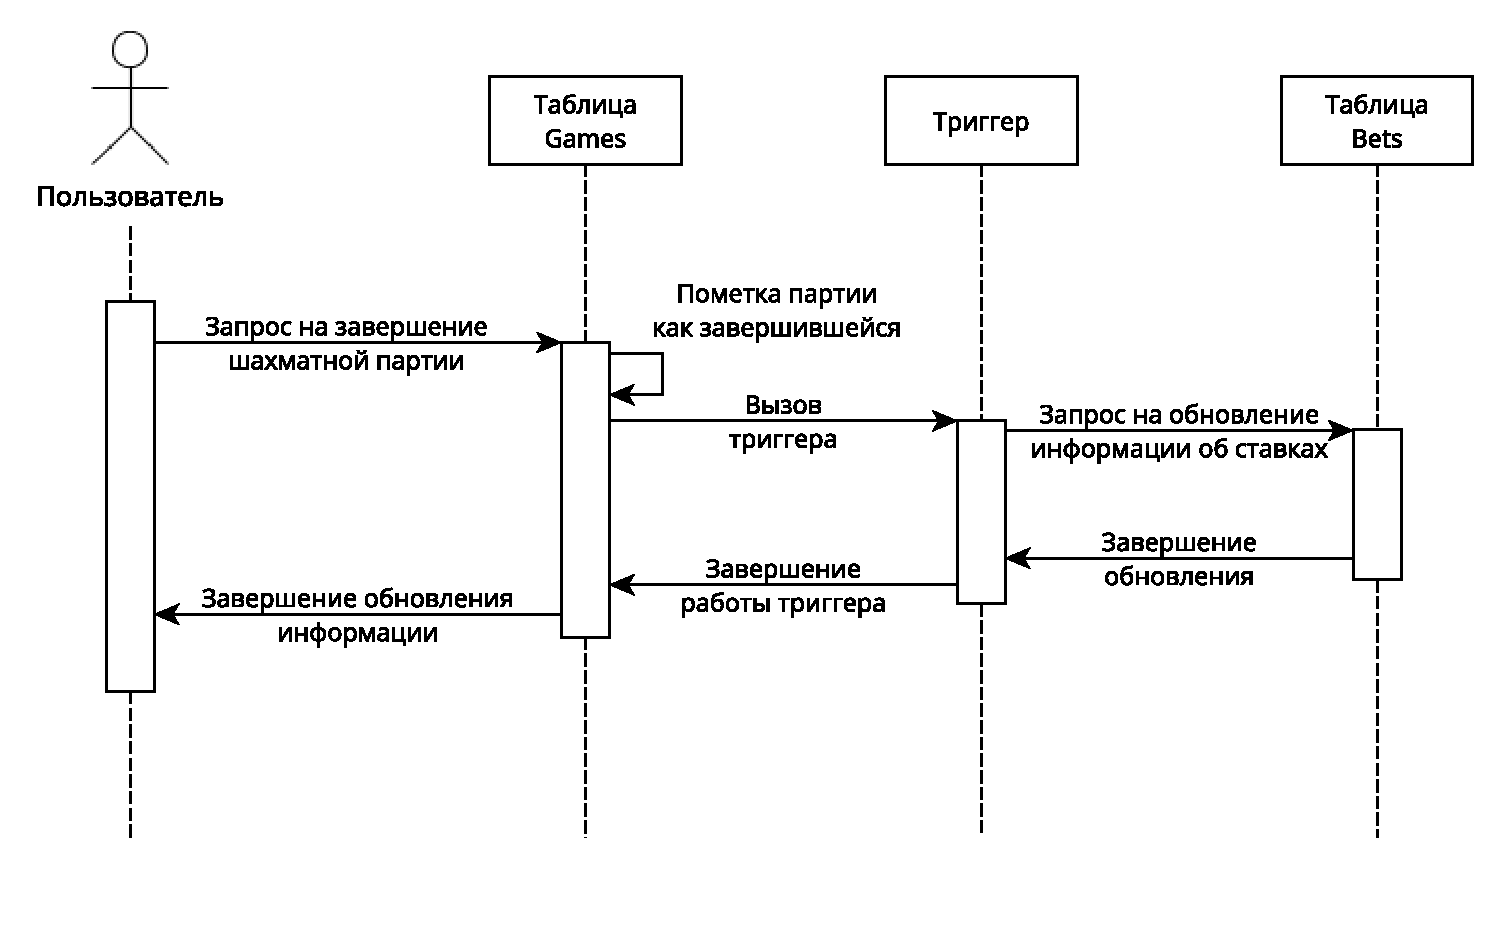
\includegraphics[width=0.7\linewidth]{bet_check_trigger_seq_diag}
	\caption{Диаграмма последовательности триггера проверки на выполнение условий ставок}
	\label{bet_check_trigger_seq_diag}
\end{figure}

\section{Структура разрабатываемого приложения}

На рисунке~\ref{common_arch} представлена структура разрабатываемого приложения.
\begin{figure}[H]
	\centering
	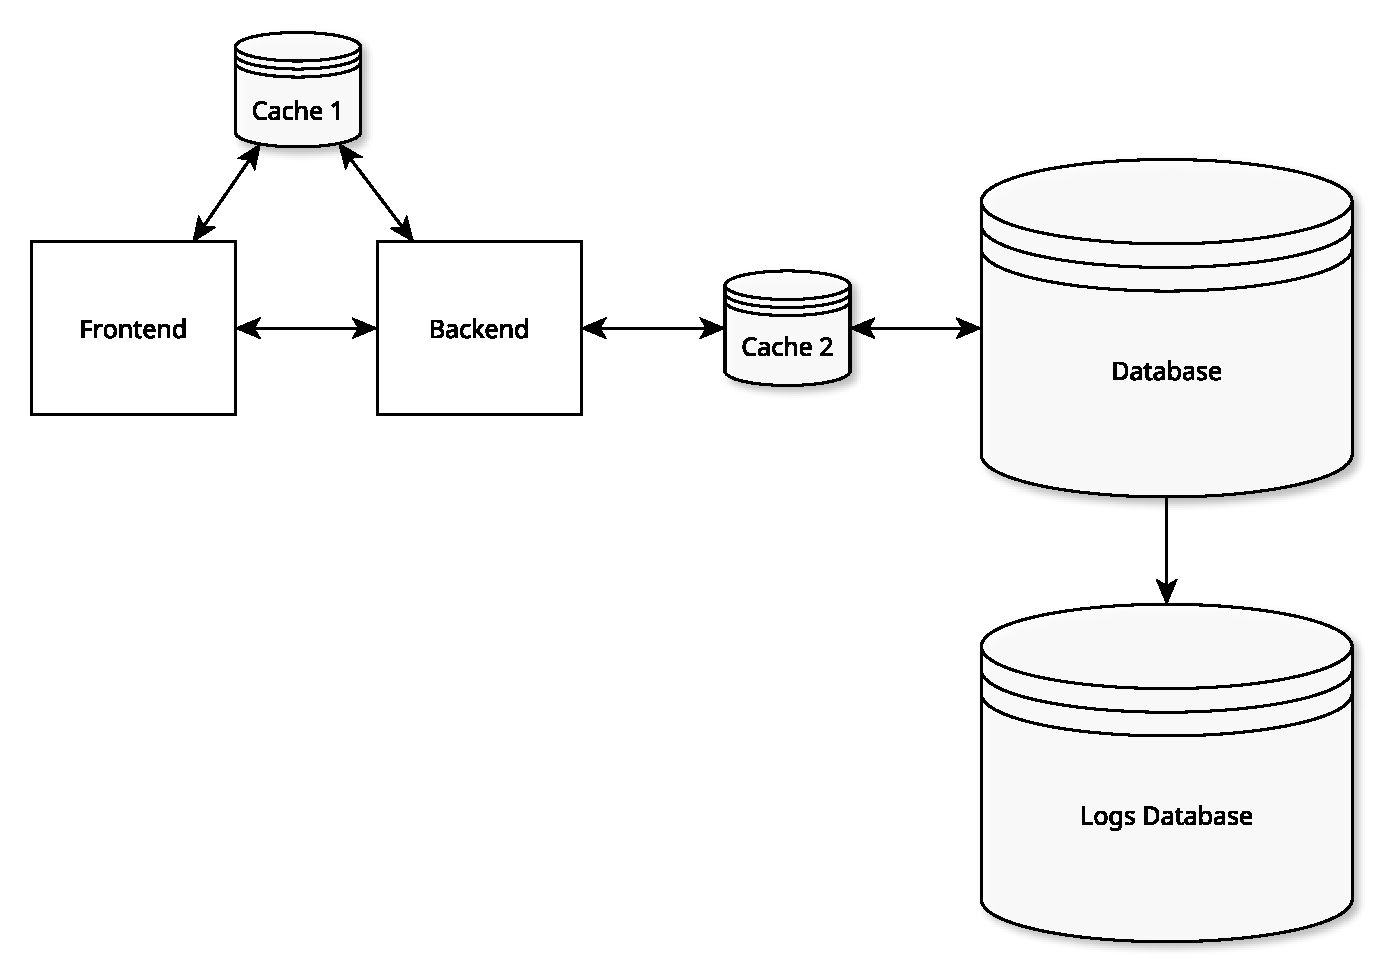
\includegraphics[width=0.7\linewidth]{common_arch}
	\caption{Структура разрабатываемого приложения}
	\label{common_arch}
\end{figure}

Логирование будет осуществляется как на стороне клиента, так и на стороне сервера. В первом случае журналирование используется для мониторинга выполнения кода приложения.
Логирование на стороне сервера осуществляется в рамках работы СУБД: любая манипуляция с базой данных будет отслежена и записана в лог-файл.

С точки зрения безопасности хранение журналов и базы данных на одном сервере не является лучшим решением: злоумышленник при попытке получения несанкционированного доступа к информации может стереть или подменить логи.
Для решения данной проблемы предлагается использовать второй сервер для хранения журналов.
%В качестве СУБД будет использована СУБД временных рядов, поскольку, в отличие от других систем, она оптимизирована для быстрого приема запросов: скорость загрузки данных не уменьшается со временем и остается стабильной~\cite{timedb}.

Для уменьшения нагрузки на сервер и увеличения производительности системы предлагается использовать два кэша: между фронтендом и бекэндом и между бэкендом и базой данных.
Первый кэш будет хранить результаты наиболее часто посылаемых запросов, второй~--- результаты больших инструкций. Программа в первую очередь будет пытаться получить данные из кэша.
При безрезультативном поиске система, ответственная за хранение кэша, посылает запрос серверу и после получении ответа обновляет данные.
%В качестве СУБД для кэширования информации предлагается использовать встраиваемые системы <<ключ-значение>>.

\clearpage
